%%%%%%%%%%%%%%%%%%%%%%%%%%%%%%%%%%%%%%%%%%%%%%%%%%%%%%%%%%%%%%%
%
%     filename  = "YourName-Dissertation.tex",
%     version   = "1.3.0",
%     date      = "2013/10/21",
%     authors   = "Gary L. Gray,
%     copyright = "Gary L. Gray",
%     address   = "Engineering Science and Mechanics,
%                  212 Earth & Engineering Sciences Bldg.,
%                  Penn State University,
%                  University Park, PA 16802,
%                  USA",
%     telephone = "814-863-1778",
%     email     = "gray@psu.edu",
%
%
%
%     		THIS THESIS TEMPLATE WAS MADE BY DR. GARY GRAY AND SIMPLIFIED FOR USE FOR ONLY A 
%                        B.S. THESIS
%%%%%%%%%%%%%%%%%%%%%%%%%%%%%%%%%%%%%%%%%%%%%%%%%%%%%%%%%%%%%%%
%
% Change History:
%
% 1.3.0	**	Added the cite package.
%
%		**	Give that the Graduate School now allows essentially
%			any line spacing, I have moved the line space setting
%			from psuthesis.cls to this driver file. Go ahead and
%			make it ugly if you want. :-)
%
%		**	Removed \addtocounter{page}{-1} after \psutitlepage is
%			executed. It made the paging of the frontmatter
%			incorrect. I can no longer remember why it was there.
%
%		**	Removed \psusigpage since the Graduate School now
%			provides the signature page.
%
%		**	Added the command \collegesubmittedto to add the College
%			in which the thesis/dissertation has been completed to
%			the title page.
%
%		**	Added instructions for documents that include a single
%			appendix since the Graduate School just hates calling it
%			``Appendix A'' is there is a single appendix.
%
%		**	Removed the fncychap package since I could not easily
%			find a way to make it work with documents that have a
%			single appendix.
%
%		**	Added the titlesec package so that the user can make the
%			format of the chapter titles a little less boring than
%			LaTeX's default.
%
% 1.2.2	**	Added some information to the main driver file (this
%			file) regarding the use of hyperref with the
%			psuthesis class. Thanks to Nathan Urban for pointing
%			out the included workaround.
%
% 1.2.1	**	Finally reproduced and fixed the problem where the
%			page number listed in the TOC for the Bibliography
%			was the last page number of the Bibliography.
%
%		**	Added 10pt and 11pt options to the document class,
%			though we have no idea why anyone would want to use
%			such insanely small font sizes since it will lead to
%			line lengths that are much too long.
%
% 1.2.0	**	Two additional class options have been added to
%			support honors theses submitted to the Schreyer
%			Honors College. These options are:
%			- honors
%			- honorsdepthead
%			See below for details.
%
%		**	We have also added the commands:
%			- honorsdegreeinfo
%			- honorsadviser
%			- honorsdepthead
%			Again, see below for details.
%
% 1.1.2	**	If you want to use the subfigure package with our
%			psuthesis class file, then you must must find the 
%			following line in the psuthesis.cls file:
%
%			\RequirePackage{tocloft}
%
%			and add the subfigure option. We have already set
%			this up for you in the psuthesis.cls file to make
%			this easy to do.
%
% 1.1.1	**	Added the fncychap package to the distribution.
%
% 1.1.0	**	The way that the thesis frontmatter and backmatter
%			is generated has been completely re-done in order
%			to be more intuitive.
%
%		**	We have added the ability to change the title of
%			the Dedication/Epigraph to anything you please.
%
%		**	In the process of changing the format of the Table
%			of Contents to conform to the inflexible rules of
%			the Grad School (the word ``Chapter'' and
%			``Appendix'' need to appear before the number and
%			letter, respectively), we have added an option to
%			the class called inlinechaptertoc that changes the
%			format of the Chapter/Appendix entries in the TOC.
%			Note that the tocloft package is now required.
%
%		**	Appendices should now start with the
%			\Appendix command rather than \chapter. See the
%			accompanying files for examples.
%
%		**	Added information regarding the Nontechnical
%			Abstract that is required of ESM students.
%
%		**	Added the fncychap package for those of you who like
%			the nice Chapter headings it provides. We like
%			Lenny, but you don't have to use it if you don't
%			want to. In addition, the other options are: Sonny,
%			Glenn, Conny, Rejne, and Bjarne
%
% 1.0.4	**	fixed the \addcontentsline entry for BibTeX within
%			the commented out text in the Bibliography section
%
% 1.0.3	**	added a sigpage option to conform to new Grad School
%			requirements
%
% 1.0.2	**	issued the \appendix command to start the appendices
%
%		**	moved the \addcontentsline for the bibliography so
%			that the bibliography now shows up on the right page
%			in the TOC
%
%		**	added some info if you use bibtex
%
% 1.0.1	**	eqlist and eqparbox are now included in the archive
%
%%%%%%%%%%%%%%%%%%%%%%%%%%%%%%%%%%%%%%%%%%%%%%%%%%%%%%%%%%%%%%%
%
% This is a template file to help get you started using the
% psuthesis.cls for theses and dissertations at Penn State
% University. You will, of course, need to put the
% psuthesis.cls file someplace that LaTeX will find it.
%
% We have set up a directory structure that we find to be clean
% and convenient. You can readjust it to suit your tastes. In
% fact, the structure used by our students is even a little
% more involved and commands are defined to point to the
% various directories.
%
% This document has been set up to be typeset using pdflatex.
% About the only thing you will need to change if typesetting
% using latex is the \DeclareGraphicsExtensions command.
%
% The psuthesis document class uses the same options as the
% book class. In addition, it requires that you have the
% ifthen, calc, setspace, and tocloft packages.
%
% The first additional option specifies the degree type. You
% can choose from:
%	Honors Baccalaureate using the option <honors>
%
% If you specify either ba or bs in addition to honors, it will
% just use the honors option and ignore the ba or bs option.
%
% The second additional option <inlinechaptertoc> determines
% the formatting of the Chapter entries in the Table of
% Contents. The default sets them as two-line entries (try it).
% If you want them as one-line entries, issue the
% inlinechaptertoc option.
%
% The class option ``honors'' should be used for theses
% submitted to the Schreyer Honors College. This option
% changes the formatting on the Title page so that the
% signatures appear on the Title page.
%
% The class option ``honorsdepthead'' adds the signature of the
% department head on the Title page for those baccalaureate
% theses that require this.
%
% The class option ``secondthesissupervisor'' should be used
% for baccalaureate honors degrees if you have a second
% Thesis Supervisor.
%
% The vita is only included with the phd option and it is
% placed at the end of the thesis. The permissions page is only
% included with the ms, meng, and ma options.
%%%%%%%%%%%%%%%%%%%%%%%%%%%%%%%%%%%%%%%%%%%%%%%%%%%%%%%%%%%%%%%
% Only one of the following lines should be used at a time.
\documentclass[draft,honorsdepthead,bs, 12pt, signature]{psuthesis}
%\documentclass[draft,secondthesissupervisor,honors, 12pt, signature]{psuthesis}
%\documentclass[draft,secondthesissupervisor,honors, 12pt]{psuthesis}

\usepackage[T1]{fontenc}
\usepackage{lmodern}
\usepackage{textcomp}
\usepackage{microtype}

%%%%%%%%%%%%%%%%%%%%%%%%%%%%
% Packages we like to use. %
%%%%%%%%%%%%%%%%%%%%%%%%%%%%
\usepackage{amsmath}
\usepackage{amssymb}
%\usepackage{amsthm}
%\usepackage{exscale}
%\usepackage[mathscr]{eucal}
%\usepackage{bm}
\usepackage{eqlist} % Makes for a nice list of symbols.
\usepackage[final]{graphicx}
\usepackage[dvipsnames]{color}
\DeclareGraphicsExtensions{.pdf, .jpg, .png}
%\usepackage{minted}


% http://www.tex.ac.uk/cgi-bin/texfaq2html?label=citesort
\usepackage{cite}

\usepackage{titlesec}

\usepackage{mathtools}                  %
\usepackage{amsthm}                     %
\usepackage{mathrsfs}                   %
\usepackage{stmaryrd}                   %
\usepackage[normalem]{ulem}             %
\usepackage[symbol,perpage]{footmisc}   %
\usepackage[numbers,sort,square]{natbib}               %
\usepackage[np,autolanguage]{numprint}  %
\usepackage{afterpage}                  %
\usepackage{setspace}                   %
\usepackage{enumerate}                  %
\usepackage{relsize}
\usepackage{booktabs}
\usepackage{epic}
%\usepackage[font={small}]{caption}  %Caption Package
\usepackage[hyphens]{url}    %Breaks up the URLs
\usepackage[section]{placeins}


%%%%%%%%%%%%%%%%%%%%%%%%%%%%%%%
% Use of the hyperref package %
%%%%%%%%%%%%%%%%%%%%%%%%%%%%%%%
%
% This is optional and is included only for those students
% who want to use it.
%
% To the hyperref package, uncomment the following line:
%\usepackage{hyperref}
%
% Note that you should also uncomment the following line:
%\renewcommand{\theHchapter}{\thepart.\thechapter}
%
% to work around some a problem hyperref has with the fact
% the psuthesis class has unnumbered pages after which page
% counters are reset.

% Set the baselinestretch using the setspace package.
% The LaTeX Companion claims that a \baselinestretch of
% 1.24 gives one-and-a-half line spacing, which is allowed
% by the PSU thesis office. As of October 18, 2013, the Graduate
% School states ``The text of an eTD may be single-, double- or
% one- and-a-half-spaced.'' Go nuts!
\setstretch{1.24}


%%%%%%%%%%%%%%%%%%%%%%%%%%%%%%%%%%%%
% SPECIAL SYMBOLS AND NEW COMMANDS %
%%%%%%%%%%%%%%%%%%%%%%%%%%%%%%%%%%%%
\graphicspath{{./Figures/}}
\newcommand{\IDH}[0]{[INSERT DATA HERE]}
\newcommand{\IFH}[0]{[INSERT FIGURE HERE]}
\newcommand{\IMH}[0]{[INSERT METHOD HERE]}
\newcommand{\IEH}[0]{[INSERT EQUIPMENT HERE]}

\usepackage{gensymb}
\usepackage{tabularx}
\usepackage{multirow}
\usepackage{caption}
\usepackage{float}
\usepackage{xr}
\usepackage{subfig}
\usepackage{ltxtable}
\usepackage[final]{listings}
\DeclareCaptionLabelFormat{blank}{}


%%%%%%%%%%%%%%%%%%%%%%%%%%%%%%%%%%%%%%%%%
% Renewed Float Parameters              %
% (Makes floats fit better on the page) %
%%%%%%%%%%%%%%%%%%%%%%%%%%%%%%%%%%%%%%%%%
\renewcommand{\floatpagefraction}{0.85}
\renewcommand{\topfraction}      {0.85}
\renewcommand{\bottomfraction}   {0.85}
\renewcommand{\textfraction}     {0.15}

% ----------------------------------------------------------- %

%%%%%%%%%%%%%%%%
% FRONT-MATTER %
%%%%%%%%%%%%%%%%
% Title
\title{Predictable Model of ABS and PLA 3D Printed Objects}

% Author and Department
\author{Kyle P. Salitrik}
\id{9-9754-3474}
\dept{Department of Engineering Science and Mechanics}

% the degree will be conferred on this date
\degreedate{Fall 2016}

% year of your copyright
\copyrightyear{2016}

% This command is used for students submitting a thesis to the
% Schreyer Honors College. The argument of this command should
% contain every after the word ``requirements'' that appears on
% the title page. This provides the needed flexibility for
% all the degree types.
\honorsdegreeinfo{for a baccalaureate degree \\ in Engineering Science}
%Include the below line if GPA > 3.2
%\honorsdegreeinfo{for a baccalaureate degree \\ in Engineering Science\\ with honors in Engineering Science}


% This is the document type. For example, this could also be:
%	Comprehensive Document
%	Thesis Proposal
\documenttype{Thesis}
%\documenttype{Dissertation}
%\documenttype{Comprehensive Document}


% This is the college to in which you are submitting the
% thesis/dissertation.
\collegesubmittedto{College of Engineering}


%%%%%%%%%%%%%%%%%%
% Signatory Page %
%%%%%%%%%%%%%%%%%%

% Input reader information below. The optional argument in [], which
% comes first, goes on the second line before the name.

%THESIS ADVISOR
\advisor[]{Dr. Albert E. Segall}%
		{Professor, Department of Engineering Science and Mechanics}


% For baccalaureate honors degrees, enter the name of your
% honors adviser below.
\honorsadviser{Dr. Lucas J. Passmore}
\honorsadvisertitle{Assistant Professor, Department of Engineering Science and Mechanics}

% For baccalaureate honors degrees, if you have a second
% Thesis Supervisor, enter his or her name below.
%\secondthesissupervisor{Mr. Nathaniel Bonha}
%\secondthesissupervisortitle{Instructor of Engineering, Penn State Fayette, The Eberly Campus}

% For baccalaureate honors degrees, certain departments
% (e.g., Engineering Science and Mechanics) require the
% signature of the department head. In that case, enter the
% name of your department head below.
\honorsdepthead{Judith A. Todd}


% Format the Chapter headings using the titlesec package.
% You can format section headings and the like here too.
\definecolor{gray75}{gray}{0.75}
\newcommand{\hsp}{\hspace{15pt}}
\titleformat{\chapter}[display]{\fontsize{30}{30}\selectfont\bfseries\sffamily}{Chapter \thechapter\hsp\textcolor{gray75}{\raisebox{3pt}{|}}}{0pt}{}{}
\titlespacing*{\chapter}{0pt}{0pt}{20pt}

\titleformat{\section}[block]{\Large\bfseries\sffamily}{\thesection}{12pt}{}{}
\titleformat{\subsection}[block]{\large\bfseries\sffamily}{\thesubsection}{12pt}{}{}


% Makes use of LaTeX's include facility. Add as many chapters
% and appendices as you like.

%Make sure you place all files here an also within the document environment
\includeonly{%
Chapter_1,%
Chapter_2,%
Chapter_3,%
Chapter_4,%
Chapter_5,%
Appendix_A,%
Appendix_B,%
}

\usepackage{listings}
%%%%%%%%%%%%%%%%%
% THE BEGINNING %
%%%%%%%%%%%%%%%%%
\begin{document}

%%%%%%%%%%%%%%%%%%%%%%%%
% Preliminary Material %
%%%%%%%%%%%%%%%%%%%%%%%%
% This command is needed to properly set up the frontmatter.
\frontmatter

%%%%%%%%%%%%%%%%%%%%%%%%%%%%%%%%%%%%%%%%%%%%%%%%%%%%%%%%%%%%%%
% IMPORTANT
%
% The following commands allow you to include all the
% frontmatter in your thesis. If you don't need one or more of
% these items, you can comment it out. Most of these items are
% actually required by the Grad School -- see the Thesis Guide
% for details regarding what is and what is not required for
% your particular degree.
%%%%%%%%%%%%%%%%%%%%%%%%%%%%%%%%%%%%%%%%%%%%%%%%%%%%%%%%%%%%%%
% !!! DO NOT CHANGE THE SEQUENCE OF THESE ITEMS !!!
%%%%%%%%%%%%%%%%%%%%%%%%%%%%%%%%%%%%%%%%%%%%%%%%%%%%%%%%%%%%%%

% Generates the title page based on info you have provided
% above.
\psutitlepage

% Generates the abstract. The argument should point to the
% file containing your abstract. 
\thesisabstract{./Material/Ancillary/Abstract}


% Generates the Table of Contents
\thesistableofcontents

% Generates the List of Figures
\thesislistoffigures

% Generates the List of Tables
\thesislistoftables

% Generates the List of Symbols. The argument should point to
% the file containing your List of Symbols. 
%\thesislistofsymbols{SupplementaryMaterial/ListOfSymbols}

% Generates the Acknowledgments. The argument should point to
% the file containing your Acknowledgments. 
\thesisacknowledgments{./Material/Ancillary/Acknowledgments}


% Generates the Epigraph/Dedication. The first argument should
% point to the file containing your Epigraph/Dedication and
% the second argument should be the title of this page. 
%\thesisdedication{SupplementaryMaterial/Dedication}{Dedication}



%%%%%%%%%%%%%%%%%%%%%%%%%%%%%%%%%%%%%%%%%%%%%%%%%%%%%%
% This command is needed to get the main part of the %
% document going.                                    %
%%%%%%%%%%%%%%%%%%%%%%%%%%%%%%%%%%%%%%%%%%%%%%%%%%%%%%
\thesismainmatter

%%%%%%%%%%%%%%%%%%%%%%%%%%%%%%%%%%%%%%%%%%%%%%%%%%
% This is an AMS-LaTeX command to allow breaking %
% of displayed equations across pages. Note the  %
% closing the "}" just before the bibliography.  %
%%%%%%%%%%%%%%%%%%%%%%%%%%%%%%%%%%%%%%%%%%%%%%%%%%
\allowdisplaybreaks{
%\pagestyle{fancy}
%\fancyhead{}
%
%%%%%%%%%%%%%%%%%%%%%%
% THE ACTUAL CONTENT %
%%%%%%%%%%%%%%%%%%%%%%
% Chapters
\chapter{Introduction}
\section{Overview}
The objective of this thesis is twofold: Primarily this study focuses on varying fabrication methods using rapid prototyping (3-D printing) including changes in extrusion/fabrication orientation, fill percentage, and material in order to create the strongest structures with minimal waste possible. Secondarily, the aim was to provide a model to predict the behavior of structures fabricated using Fused Deposition Modeling under the various parameters tested. Beam specimens were designed in Solidworks and tested using a custom fixture designed and built for the purpose. All of the tensile test specimens were also designed using Solidworks and were intended to be tested according to the guidelines set forth in the ASME Standard Test Method for Tensile Properties of Plastics. \par
	In addition to the varied fabrication factors listed above the rapid prototyping was done using two different materials commonly found in the industry: PLA and ABS plastics. After an optimal method was discovered in fabricating both the PLA and ABS tensile test specimens, more complex structures were created and evaluated using both materials. The next step after completing the initial tensile testing was to create an I-Beam and predict the displacement based on the bending strength of the square and rectangular specimens. Finally, tensile test specimens were intended to be created and tested according to ASTM D638 for type I specimens \citep{ASTMNorma2004}. All test specimens used in the study were printed using Ultimaker 2 3D printer units, pictured in figure \ref{fig:Printer_Clean}.
	
	\begin{figure} [H]
		\centering
		\caption{Ultimaker 2 Printer}
		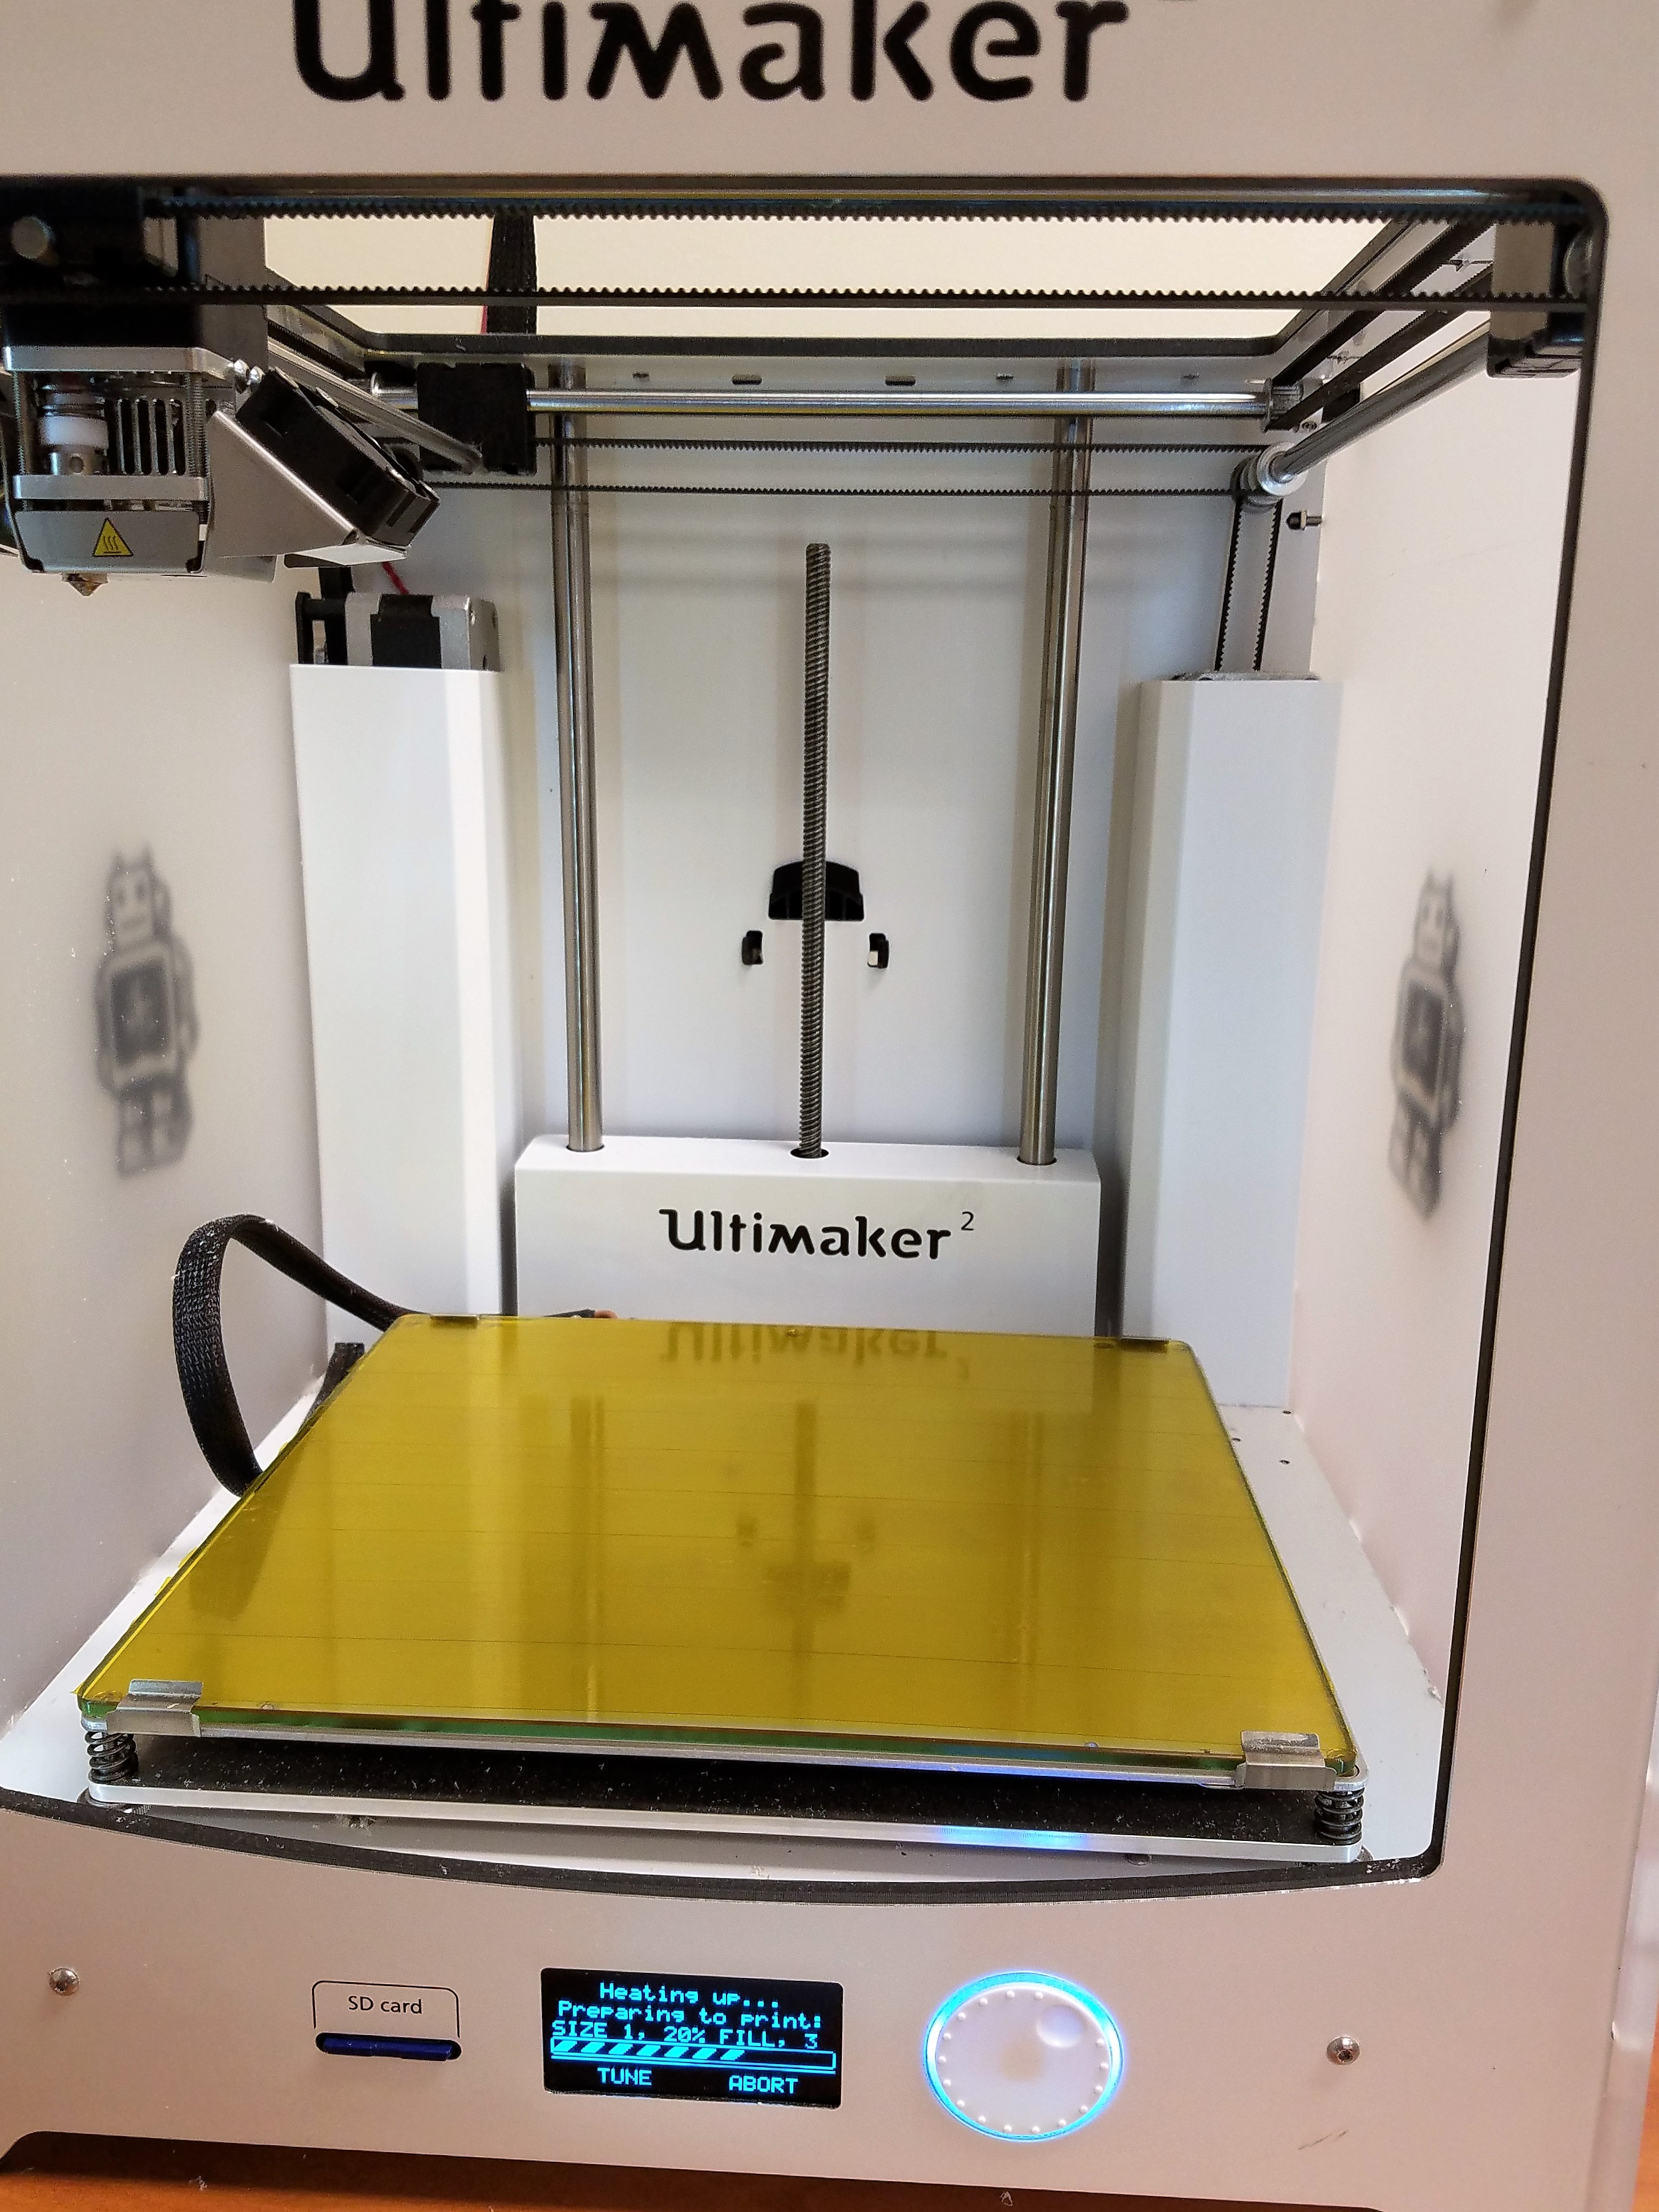
\includegraphics[width=.5\textwidth]{Printer_Clean}
		\label{fig:Printer_Clean}
	\end{figure}
	
\section{Impacts of Research}
	The outcome of the research could provide industries with a significantly cheaper alternative to creating prototypes with expensive metals such as aluminum in order to run real-world tests and showcase their products. Using 3-D printed plastics also creates less waste due to the fact that additive manufacturing methods only require the amount of material needed to create the object, while machining methods could force one to purchase significantly more material than necessary in order to create a part, also contributing to savings. Another benefit to using rapid prototyping is the ability to fairly easily create complex structures that may require expensive outsourcing or costly development methods in order to create a prototype out of a machined metal. Furthermore, using ABS or PLA plastics can be more sustainable due to the fact that the plastics can be recycled into filament for 3-D printing, presumably cheaper than metals.
	
\section{Methods Evaluated}
		The following table outlines the varied fabrication methods used to determine an optimal tensile test specimen for extruded plastics in comparison to metal test specimens. Full detail on specimens and tests will be covered in Chapter 4. Testing was done in three phases with three different purposes:
	\begin{table} [h]
		\centering
		\begin{tabular}{ l l l }
		\noalign{\hrule height 2pt}
		Phase I & Phase 2 & Phase 3 \\ \hline
		Determine Elastic Moduli & Predict Behaviour \& & Determine UTS \\ 
		of ABS \& PLA &Study Print Orientation & of Tensile Specimens\\ \hline
		\end{tabular}
		\caption{Test Phases}
		\label{tab:TestPhases}
	\end{table}
	
	Phase I consisted of designing three sizes of square and rectangular beams such that the beams of each respective size had an identical cross-sectional area. To help rule out fabrication anomalies, three copies of each beam were printed using PLA plastic. The 9 specimens were then tested in a custom-built bending stress test fixture. Data was collected using PASCO electronic sensors and was used to determine an elastic modulus for the specimens. The 9 specimens were also printed with three different in-fill densities in order to determine the effects of density on the strength of the beams. Next, the entire fabrication and testing was repeated using ABS plastic.\par
	In Phase II, predictions were made from the average modulus of elasticity found in Phase I. To do this, I-beams were printed in three different print orientations with three samples each and the top flange, bottom flange, and web were measured. Using these measurements, the Moment of Inertia of each beam was calculated and used along with the average modulus to determine the estimated deflection of the beam when a 40N force was applied. Once this was completed, the beams were tested using the bending stress test fixture used in Phase I. The logged data was compared to the predicted strengths of the beams to determine the accuracy of one's ability to predict structural behavior. Finally, the average modulus of the beams were calculated and compared to the modulus of elasticity of PLA in order to determine the effects of layer orientation on the strength of an object.\par	
	Phase III was intended to be performed by printing out ASME standard conforming plastic tensile test specimens using 100\% in-fill density, along with varying print orientations in the same manner as the I-beams. The specimens would have been tested using a specially designed grip extension for the tensile test machine, as one of the limiting factors of 3D printing is the maximum fabrication size. This data would have been compared to the tensile test results of $\frac{1}{8}$ inch thick sheets of aluminum cut out to according to ASTM standards in order to determine if there was a possible print orientation that behaves comparably to a linear, homogeneous, isotropic material.
	
\section{Terminology Used in this Thesis}
	As a preface to understanding the terminology that will be used throughout this study. Figure \ref{fig:Fill_definition} illustrates what is meant by fill density. The solid hatched border of the squares represents the wall thickness, which is discussed later but is important to note. Figure \ref{fig:Layer_definitiion} defines what is meant when layer orientation is mentioned. For all tensile test studies, the terms Longitudinal and Transverse are used knowing that the force is applied to the face shown by the square cross section in figure \ref{fig:Layer_definitiion}.


	\begin{figure} [H]
		\centering
		\caption{3D Printer Fill Density }
		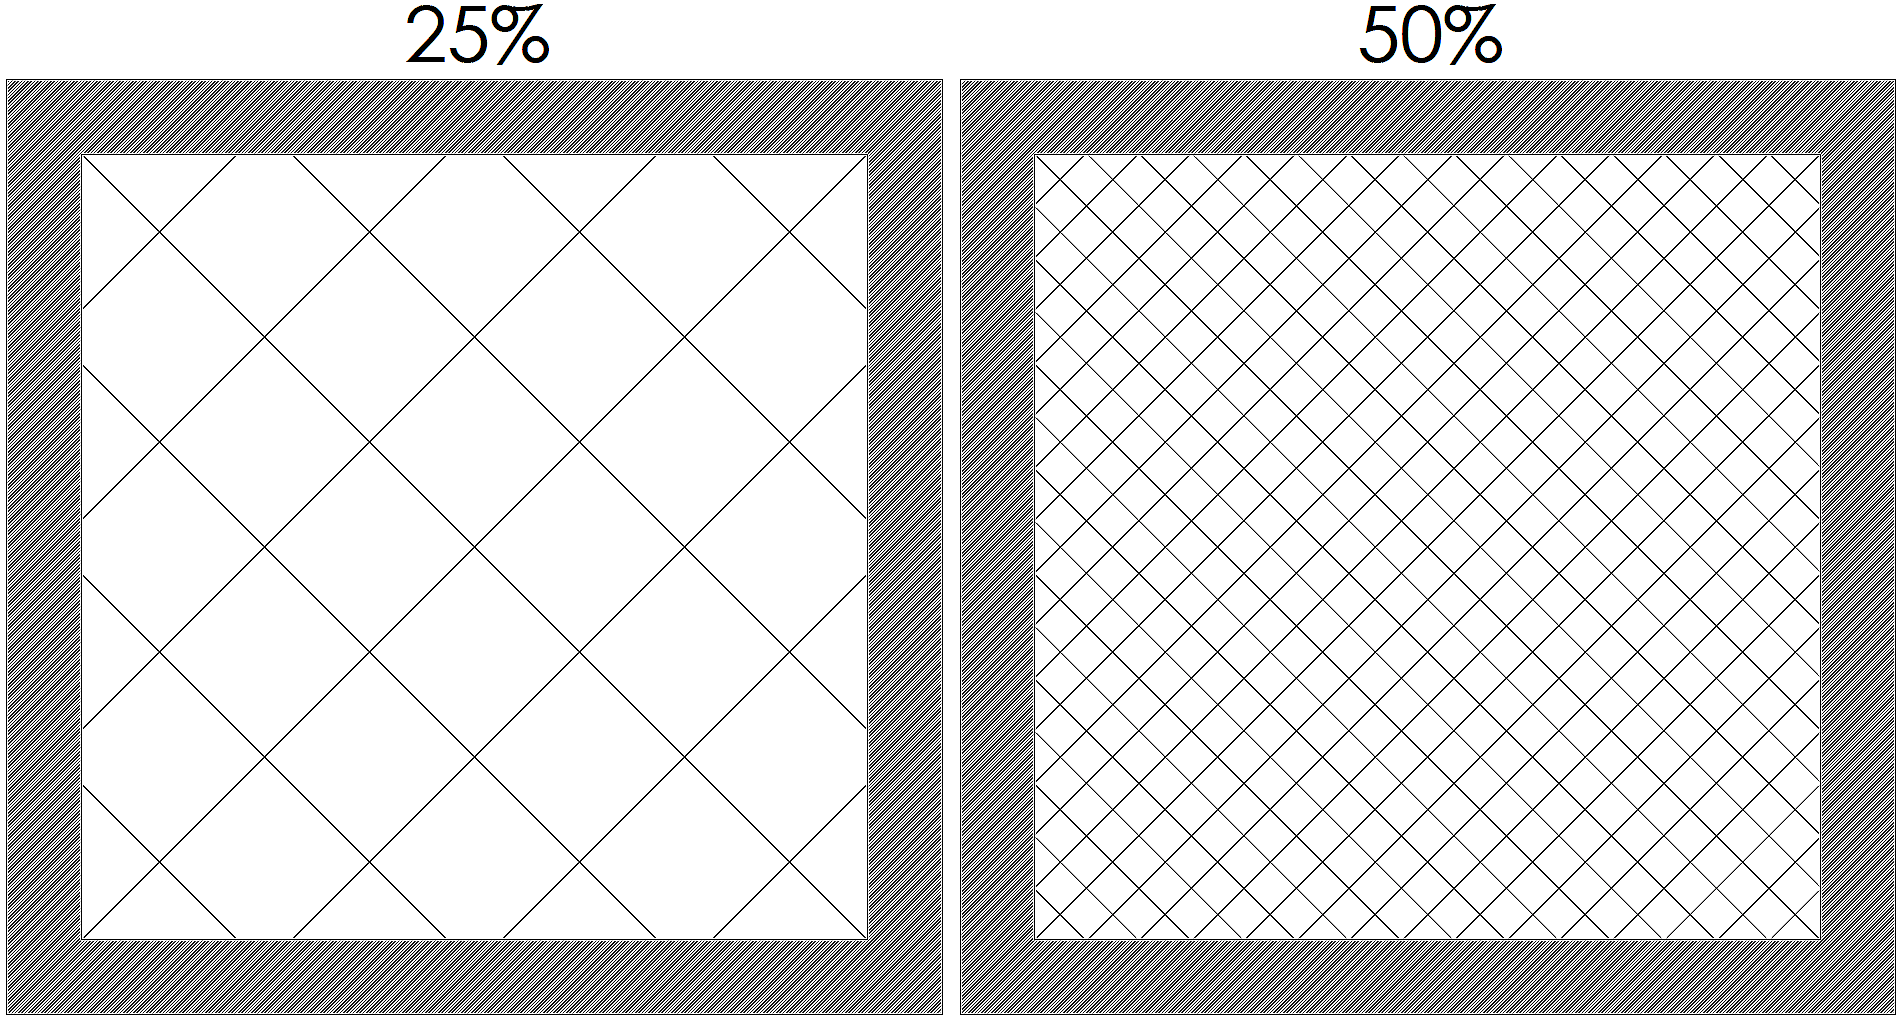
\includegraphics[width=\textwidth]{Definition_Fill}
		\label{fig:Fill_definition}
	\end{figure}
	\begin{figure} [H]
		\centering
		\caption{Print Layer Orientation}
		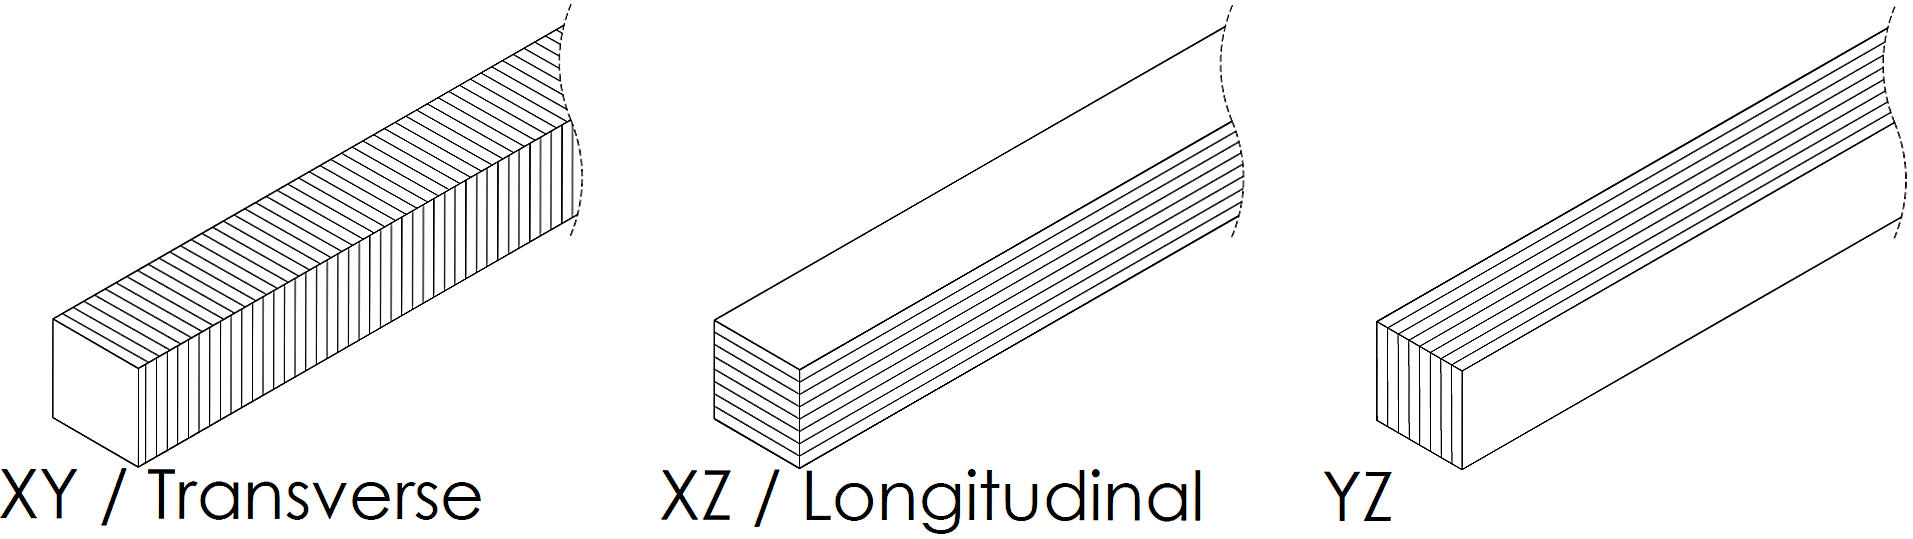
\includegraphics[width=\textwidth]{Definition_Layers}
		\label{fig:Layer_definitiion}
	\end{figure}
\chapter{Literature Review}
%-------------------------------------------------------------------------
\section{Background of Additive Manufacturing}
\subsection{Types of 3D Printers}
	There exist many types of additive manufacturing devices that exist \citep{Gross2014, Savini2015}. Today, when one thinks of a 3D printer, the archetype of Fused Deposition Modeling (FDM) type comes to mind. This is due to the popularity of FDM printers with mainstream culture because the ease of access to these printers and their relatively affordable prices compared to other 3D printing devices \citep{Gross2014, Savini2015}. However, the idea of additive manufacturing dates back to the 1970s where patents were first filed for ideas of AM techniques \citep{Savini2015}.\par
		The first instance of additive manufacturing, or 3D Printing, was the creation of a small cup using Stereolithography (STL) and was invented by Charles Hull in August of 1984 \citep{Savini2015}. Hull developed the method of additive manufacturing (AM) by using a laser to heat a base located in a resin bath in order to harden and fuse the resin into a solid shape, the bed would then lower and the process would start again until the final object was created \citep{Gross2014}. Along with taking a matter of months to make a 5cm tall cup \citep{Savini2015}, another drawback of this --- and many other --- AM method is the limited height of a print \citep{Gross2014}. This was overcome by creating STL manufacturers that held the bed above the resin bath in order to increase print volume significantly \citep{Gross2014}.\par
		Another early method of additive manufacturing was also developed in the late 1980s called Laminated Object Manufacturing (LOM) \citep{Savini2015}. This technique of 3D printing consists of cutting cross-sectional layers of a material, usually with a laser, and laminating the layers together \citep{Savini2015}.\par
		In 1989, a technology using the same Inkjet principles already used by 2D printers was developed and trademarked by MIT and the term "3D Printing" was finally coined \citep{Savini2015}. During the process of Inkjet AM the device lays a level bed of powder and then passes over it either depositing a binding liquid that solidifies the particles into a layer or uses a laser to melt the particles into a cross-section; the bed then lowers and starts the process over again until the object is built \citep{Gross2014}. Also, in 1989, Selective Laser Sintering was developed, which is a technique similar to the inkjet printing where a laser is used to harden powdered material into a layer of an object \citep{Savini2015}.\par
		Returning to what people commonly think of when they hear the term "3D Printer," Fused Deposition Modeling was also developed in the late 80s. The process of building an object with this method starts by melting a filament (usually a thermoplastic) and extruding it onto a base, layer by layer, until the object is formed \citep{Savini2015}. FDM printers would go on to facilitate the creation of two major projects run by universities and jump start their popularity. In 2005, the Replicating Rapid Prototyper --- or Rep Rap --- project was started by A. Bowyer, a professor at the University of Bath \citep{Savini2015}. The RepRap printers were designed using Open Source hardware such as Arduino micro-controllers and software, with the idea of being able to 'replicate' themselves by printing as many parts of themselves as possible \citep{Savini2015}. The Hammond Engineering Building at Penn State University Park has its own 3D Printing lab that is mostly powered by Rep Rap printers. The second project was started by Cornell in 2006 and was dubbed Fab@Home \citep{Savini2015}.\par
		Since the 1980s, there have been over 20,000 patents filed related to additive manufacturing techniques \citep{Savini2015}. Today, common desktop 3D printers such as the Ultimaker 2+, Witbox 2, and Lulzbot TAZ 6, amongst others, can print filaments containing metals, carbon fiber and even wood. However, Hull's Stereolithography development brought with it the gold standard for the files that nearly all additive manufacturers use even to this day, the .STL format, which stands for Standard Tessellation Language \citep{Gross2014}. These files contain the information of an object designed with 3D CAD software, broken down into triangles; to use these files with a 3D printer, they must first be interpreted by a slicing program that 'slices' the object into layers and produces an output file that can be read as instructions by the 3D printer, usually a .gcode file \citep{Savini2015, Gross2014}.

%-------------------------------------------------------------------------
\subsection{Difficulties of Extrusion Printing}	
	There are, however, downsides to printing using filament extrusion printers. Some types of plastic, such as ABS, require the use of a heated bed in order to help prevent the structure from warping and lifting. Another point of failure is first layer adhesion. If the first layer would lift from the printing base for some reason, that could cause the entire print to become offset or warped.Most printers are also unable to print objects with large gaps or 90 degree bends without a supporting structure, creating waste and possible defect sites during removal.\par
	Internal stress is another risk of FDM methods for 3D printing. During the process of printing, as a layer cools, it has the potential to shrink and induce a small amount of internal stress is that can build up over time. This can lead to warped structures, failed prints and even points of catastrophic failure if the print orientation is parallel to the direction that external forces are applied to the object.\par
	The layering of material is also important to us in our exploration of the mechanical properties of rapid prototyped structures. The layering creates many points of failure on the structure when faced with forces parallel to the direction of layering. The layers will, for lack of a better term, delaminate and fail at much lower forces than if they were exerted perpendicular to the layering. Transverse shear stress is another point of consideration when studying the layered structures.\par

%-------------------------------------------------------------------------
\subsection{Uses of 3D Printers}
	Additive Manufacturing has applications in nearly every market space that consists of physical goods. According to Savini, additive manufacturing is already used regularly in the aircraft, automobile, electronics, robotics, tool, toy, jewelry, food, prosthetic and tissue engineering industries \citep{Savini2015}. Gross, et al. go into detail on industry uses of 3D Printing regarding electronics and bioengineering. There is currently ongoing research and development in printing bone and dental structures, as well as scaffolds for organ and vascular tissue \citep{Gross2014}.\par
	Of particular interest to bioengineering tissue are the properties of bioresorption --- the capability of the body to absorb a substance --- and biocompatibility, whether or not the body will accept or reject the object \citep{Gross2014}.\par
On the topic of biocompatibility, Gross, et al. reported that tissue scaffolds made from tissue that was sourced from the person had a higher acceptance rate by the body than a foreign implant \citep{Gross2014}. The porosity and biodegradability of printed bone grafts is also an interesting area of research as adhesion to current bone structures is dependent on the ability of the natural bone to adhere to the printed graft by growing into and/or through the pores \citep{Gross2014}. Another use of 3D printing in the medical field is to gain insight into the patient's anatomy before surgery that may not have been apparent from MRI or x-ray imaging by reconstructing the anatomy in a physical object \citep{Gross2014}. Surgeries ave also been simulated using this method \citep{Gross2014}.\par
	In the field of electronics, both lithium ion batteries and conductive copper have been fabricated using additive manufacturing, allowing the creation of PCBs using simpler fabrication methods \citep{Gross2014}. Even apparel companies are entering the market using additive manufacturing techniques to create customized products \citep{Weller2015}. This leads into the ways that 3D printing is disruptive to current market structures and how the mass adoption of 3D printing could affect the economic climates.\par

%-------------------------------------------------------------------------
\section{Economic Impacts}
	The introduction of additive manufacturing to markets could potentially to cause significant changes in the ways consumers perceive, consume, develop and even produce goods. Firms that employ additive manufacturing methods have the potential benefits of increasing their share(s) of their current market(s) as well as the potential to enter other markets with little to no extra costs \citep{Weller2015, Rayna2016}. This section will provide an insight into the potential economic impacts of widespread additive manufacturing being employed into the current market. According to Weller, et al. there are four main markets that appeal to additive manufacturing: "small production output, high product complexity, high demand for product customization, and spatially remote demand for products" \citep{Weller2015}.

%-------------------------------------------------------------------------
\subsection{Market Entry, Expansion, and Disruption}
	Additive manufacturing provides a unique advantage of being a relatively low-cost market entry method due to the fact that, excluding the 3D printing devices themselves, a company does not need to invest in tools or costly molds for mass production \citep{Weller2015, Rayna2016}. Another major benefit of businesses employing additive manufacturing is that there is no up-front costs for production runs or storage (other than the material for production), allowing the company to focus their assets on other aspects of the business such as advertising and product development \citep{Rayna2016}. Then, when a firm finally receives orders, they can print and ship the products on demand to the consumer \citep{Rayna2016}. This allows small firms and start-ups to potentially enter markets that were once out of reach due to the high cost of starting production using current mass production methods \citep{Rayna2016}.\par
	The increase in market competition and the low cost of production for small batches of products allows the new firms to potentially disrupt the current markets and drive down the cost of currently existing products and benefit consumers \citep{Weller2015, Rayna2016}. in an example given by Rayna, et al. additive manufacturing methods allowed a business to significantly cut production time and cost of pump castings for U.S. nuclear submarines \citep{Rayna2016}. In reality there is still a place for traditional manufacturing methods. Small economies of scale allow firms to thrive using additive manufacturing, however at this point, methods like injection molding are still significantly less expensive for large production volume \citep{Weller2015}.

%-------------------------------------------------------------------------
\subsection{Product Development}
	The first significant, and potentially obvious, advantage of additive manufacturing in consumer product offerings is the ability of a firm to provide highly customized products at little to no cost to the firm and without the need to purchase new molds or tools for new products as with traditional manufacturing methods \citep{Weller2015, Rayna2016}. Markets that demand similar, yet unique products benefit from additive manufacturing because there is no cost in changing what is being produced as the only difference is using a different CAD file \citep{Weller2015, Rayna2016}. Lead times are also significantly reduced for custom small batch or single run production due to the flexibility of the additive manufacturing systems \citep{Weller2015, Rayna2016}. In essence, as put by Weller, additive manufacturing enables product "flexibility and customization for free" \citep{Weller2015}. These customization methods using 3D printing techniques have already been employed by Nike in 2013 by offering customized football cleats \citep{Weller2015}. These customized products could potentially lead to the ability for the firm to make a larger profit due to the perceived worth of a personalized product being higher than a mass produced one \citep{Weller2015}.\par
	Rapid prototyping also allows firms to increase their market share by significantly reducing the time it takes to go from concept to production \citep{Weller2015, Rayna2016}. The use of rapid prototyping enables firms to create new product iterations with minimal costs \citep{Weller2015}. However, product prototyping is not limited to any specific industry. The flexibility of additive manufacturing allows companies to acquire competencies in markets that they were previously unable to access, tying back to the ability of AM to allow low market entry costs \citep{Rayna2016}. Along with rapid prototyping, rapid tooling is another very useful tool for companies. Rapid tooling allows the company to make customized "tools, jigs, hardware and molds" for their products and increase production by having the exact tools they need \citep{Rayna2016}.\par
	A third major advantage of 3D printing technologies is the ability to create very complex products with no special tools or equipment \citep{Weller2015}. This ability to build complex structures that would normally require a significant amount of money invested in special tools or paying someone to manually manufacture is provided, essentially, for the same cost of producing a very simple object \citep{Weller2015}. Along the same lines of cost savings, multi-part products could potentially be built fully or partially assembled using AM in order to cut costs on paying workers for assembly \citep{Weller2015}. The free complexity and potential one-step production are both appealing to new entrants to market and current firms alike.

%-------------------------------------------------------------------------
\subsection{Crowdsourced Economy}
	3D Printing also has a history of crowdsourcing for innovation and development \citep{Rayna2016}. There are many outlets for individuals to provide or procure 3D printing services either from a company or another individual that owns a 3D printing device \citep{Rayna2015}. The first of these was Ponoko, followed shortly by Shapeways and Thingiverse \citep{Rayna2015}. This crowdsourced market allows the potential for companies to create print-at-home, or home fabricated, products much like tickets used by the transport and entertainment industries \citep{Rayna2015}. Additive manufacturing platforms also enable consumers to insert themselves at any stage of the production process from concept, to design, and now finally production \citep{Rayna2015}. The hope of these platforms and the interaction between consumers and industries is to enable more innovation by allowing individuals to creatively come up with solutions to issues with products, ultimately creating competition within the market \citep{Rayna2015, Rayna2016}.

%-------------------------------------------------------------------------	
\section{Prior Mechanical Testing on 3D Printed Objects}
%-------------------------------------------------------------------------
\subsection{Fused Deposition Modeling}
	As Fused Deposition Modeling (FDM) is one of the most common types of 3D printing methods use, nearly every 'personal' 3D printer that can be found on the market for $\approx \$2500$ or less are FDM printers. While it is possible to get high quality parts from these machines, it is not without effort as many defects appear in prints from voids, delamination, and deformation to under-extrusion, mis- or over-stepping of the stepper motors and electronic failures. The quality of prints significantly depends on the type of stepper motors used, the thread pitch of the threaded rods, and the stepper motor controller as these components determine how far the printer head or bed moves with one step. Although not covered in this thesis, one observation during the printing of the test specimens used was the consistency of the quality of prints due to user error and/or power failure.

%-------------------------------------------------------------------------
\subsubsection{ABS}
	Testing on ABS was relatively more prevalent than PLA, and more data could be found on the subject. Both Novakova-Marcincinova and Perez noted that they followed ISO and ASTM standards, respectively: Novakova-Marcincinova, et al. followed EN ISO 527-1 and 527-2 for Plastics Testing Methods, while Perez, et al. followed ASTM D638 and used Type V test specimens \citep{Novakova-Marcincinova2013, TorradoPerez2014}. Wendt posed concerns with the currently available standards as they do not account for the anisotropy and/or heterogeneity imposed by additive manufacturing and proposes that a better standard be developed \citep{Wendt2015}.\par
	Ahn reported that due to the nature of how FDM parts are constructed, they show anisotropic behavior of their modulus in perpendicular axes, which is intuitively predictable \citep{Ahn2003}. Perez also stated that this was one of the major flaws of Additive Manufacturing \citep{TorradoPerez2014}. During testing, Ahn discovered that the printing raster angle and air gaps between filament layers had the most significant impact on an objects strength \citep{Ahn2003}. Ahn's team printed specimens that had layers printed purely parallel, purely perpendicular, at 45\degree alternating 90\degree between layers, and 90 degrees alternating between layers \citep{Ahn2003}. When performing tensile tests they noticed that the specimens printed with 45\degree angles sheared along a 45\degree angled plane with respect to the loading direction while the parallel and perpendicular layers failed perpendicular to loading direction \citep{Ahn2003}. The model that Ahn came up with during their investigation could predict the behavior of samples fairly well \citep{Ahn2003}. The following table summarizes the mechanical properties of Ahn, et al.'s specimens.

	\begin{table} [h]
		\centering
		\begin{tabularx}{\textwidth}{| X | l | X | l |}
		\noalign{\hrule height 2pt}
    		\multicolumn{4}{|c|}{\textbf{Mechanical Properties of Ahn's ABS Specimens}}\\ \hline
		Longitudinal Strength & 22.1 MPa & Longitudinal Modulus & 25.1 GPa\\ 
		Transverse Strength & 14.4 MPa & Transverse Modulus & 9.49 GPa\\ 
		Shear Strength & 10 MPa & Shear Modulus & 1.41 GPa\\ 
		Poisson's Ratio & 0.367 & &\\ \hline
		\end{tabularx}
		\caption{ABS Specimen Mechanical Properties from Ahn \citep{Ahn2003}}
		\label{tab:AhnABS}
	\end{table}
	\par
	Perez's group also performed similar testing on Type V ASTM D638 tensile specimens, as stated before \citep{TorradoPerez2014}. A few more details were provided by Perez, such as the speed at which the tests were performed: 10 mm/min and the values were based on a 5 sample average \citep{TorradoPerez2014}. Perez also investigated the effects of print layer orientation on ABS pieces, printing samples with layers perpendicular to the load direction and parallel to the loading direction \citep{TorradoPerez2014}. The horizontally printed specimens were closer in material properties to the specimens created by Ahn, while the vertically printed specimens --- the ones with layers perpendicular to the loading direction --- were significantly weaker, with nearly half of the strength of the horizontally printed specimens \citep{TorradoPerez2014}. The data provided by Perez follows.
	
	\begin{table} [h]
		\centering
		\begin{tabularx}{\textwidth}{| l | l | X | }
		\noalign{\hrule height 2pt}
    		\multicolumn{3}{|c|}{\textbf{Mechanical Properties of Perez's ABS Specimens}}\\ \hline
		Parameter & Longitudinal & Transverse \\ \hline
		Strength & 28.4 MPa & 14.1 MPa \\
		Modulus & 1530 MPa & 1190 MPa \\
		Elongation & 4.5\% & 1.5\% \\ \hline
		\end{tabularx}
		\caption{ABS Specimen Mechanical Properties from Perez \citep{TorradoPerez2014}}
		\label{tab:PerezABS}
	\end{table}

%-------------------------------------------------------------------------
\subsubsection{PLA}
	ABS is usually preferred over PLA in manufacturing settings due to the brittleness of PLA. Wendt, et al. investigated the mechanical properties of PLA printed objects in 2015 and provided useful data for comparison. Wendt noted that most failures were due to manufacturing defects in the tested samples \citep{Wendt2015}. Suggestions were given on how to avoid common defects: gas bubbles were found less commonly when the extrusion temperatures were reduced and out of plane distortions were easier to control when the print bed was properly leveled \citep{Wendt2015}. Another suggestion for avoiding out of printing plane distortions was to design the path that the extrusion would follow to facilitate heat dissipation \citep{Wendt2015}. Along with testing their test specimens Wendt, et al. tested the raw PLA filament and the following results were found.
	
	\begin{table} [h]
		\centering
		\begin{tabularx}{\textwidth}{| X | X |}
		\noalign{\hrule height 2pt}
    		\multicolumn{2}{|c|}{\textbf{Mechanical Properties of PLA Filament}}\\ \hline
		Testing Stress & 8 -- 13 MPa \\ 
		Modulus of Elasticity & 1775 -- 2392 MPa\\
		Tensile Strength & 43 $\pm$ 2 MPa\\ \hline
		\end{tabularx}
		\caption{PLA Filament Mechanical Properties from Wendt \citep{Wendt2015}}
		\label{tab:WendtPLAF}
	\end{table}
	\par
	Wendt stated that the thickness of the printed specimens varied from the specified values significantly \citep{Wendt2015}. Table \ref{tab:WendtPLAS} references data taken from Wendt's study with the Applied Stress adapted from applied force \citep{Wendt2015}.
	
	\begin{table} [h]
		\centering
		\begin{tabularx}{\textwidth}{| X | X | X |}
		\noalign{\hrule height 2pt}
    		\multicolumn{3}{|c|}{\textbf{Mechanical Properties of PLA Specimens}}\\ \hline
		Applied Stress & 69.0 -- 70.9 MPa & 69.8 MPa avg.\\ 
		Modulus of Elasticity & 2086 -- 2249 MPa & 2159 MPa avg.\\
		Tensile Strength & 42.9 -- 44.1 MPa & 43.4 MPa avg\\ \hline
		\end{tabularx}
		\caption{PLA Specimen Mechanical Properties from Wendt \citep{Wendt2015}}
		\label{tab:WendtPLAS}
	\end{table}
	\par
	One interesting result is that the variance of the modulus of elasticity was not as significant in the printed parts as it was in the raw filament, which may point to an improvement in consistency of build materials once the part is extruded. The tensile strength, however, seemed to remain fairly constant from filament to printed part in this case.
	
%-------------------------------------------------------------------------
\subsubsection{Other Materials}

	While PLA and ABS are two of the most common materials, especially for the hobbyist market, there are many other types of FDM filament are available. Two studies investigated here involved polycarbonate and carbon fiber reinforced thermo-plastic (CFRTP) 3D printed objects \citep{Lipina2015, Klift2016}. Lipina, et al. studied fractures in polycarbonate structures due to high torques being applied to bolts on fixtures made of polycarbonate as well as fatigue failures \citep{Lipina2015}. Polycarbonate is of particular interest due to its' use in the automotive and aircraft industries \citep{Lipina2015}. The samples made by the group were compared to the manufacturer given properties and found the tensile strength to be about 81\% of the prescribed tensile strength.\par
	The investigation by Klift, et al. into CFRTP structures was more exhaustive than the polycarbonate study and involved determining how much of the strength of composite materials is preserved when used in additive manufacturing \citep{Klift2016}. They found that the strength of the part was directly related to the size of the objects being printed, noting that increases in print size correlated to a loss in overall strength of the print \citep{Klift2016}. Due to the difficulty of manufacturing layers of continuous composite fibers, the print trajectories were varied in order to minimize the number of discontinuities in the carbon fiber \citep{Klift2016}. Klift found that when following the rule of mixtures for composites, specimens with more layers of CFRTP deviated more from the predicted strength than those with fewer layers \citep{Klift2016}.\par
	Three types of samples were tested in the study: one group of pure nylon, a second group with two layers of carbon fiber reinforced nylon in the middle layers of the print, and the third and final group with six layers of CFRTP in the center \citep{Klift2016}. Tests were performed at a strain rate of 2mm/min \citep{Klift2016}. They found that the CFRTP samples failed, following suit with other types of FDM failures, where discontinuities or manufacturing defects were located \citep{Klift2016}. The results from Klift, et al. are re-summarized below.

	\begin{table} [h]
		\centering
		\begin{tabularx}{\textwidth}{| l | X | X |}
		\noalign{\hrule height 2pt}
    		\multicolumn{3}{|c|}{\textbf{Mechanical Properties of PLA Specimens}}\\ \hline
		& 2 CFRTP Layers & 6 CFRTP Layers\\ 
		Modulus of Elasticity & 231.4 GPa & 173.24 GPa\\
		Ultimate Tensile Strength & 128-171 & 370-520 MPa \\ 
		Strain & 1.3\% & 1.3-2.0\& \\ \hline
		\end{tabularx}
		\caption{CFRTP Specimen Mechanical Properties from Klift \citep{Klift2016}}
		\label{tab:KliftCFRTP}
	\end{table}
\par
%-------------------------------------------------------------------------
\subsection{Stereolithography (SLA)}
	Although it is not a method being studied by this thesis, Stereolithography continues to be a fairly common additive manufacturing method and provides another point of reference for the mechanical properties of layer based manufacturing. According to Alharbi, SLA is one of the more present 3D printing methods used in dentistry \citep{Alharbi2016}. Alharbi's team studied the effects of build direction on compressive strength in cylinders made from a specialized dental material called Temporis \citep{Alharbi2016}. Intuitively, specimens with layers printed perpendicular to the applied loading had a significantly higher compressive strength than those that were printed with layers parallel to the loading direction; 297 MPa for perpendicular specimens vs 257 MPa for parallel \citep{Alharbi2016}. As with FDM, they concluded that the bonding between layers of additive manufactured parts is weaker than the layer of the material itself \citep{Alharbi2016}.\par
	Adamczak, et al. however, studied the uncertainty in the strength of 3D printed objects using SLA. Following ASTM D638, they chose to investigate the Type I specimens, as opposed to the Type V specimens used by Perez, et al. \citep{Adamczak2014, TorradoPerez2014}. They stated that determining the mechanical properties of products for every additive manufacturing process would be difficult, but knowing the uncertainty/deviation in cross-sectional geometry of test specimens would allow one to more accurately determine the potential range of the strength of a manufactured object \citep{Adamczak2014}. \par

\subsection{Directed Energy Deposition}
	One final study of interest used a method of additive manufacturing known as directed energy deposition. It performs similarly to FDM, however instead of a nozzle being heated to the melting point of a plastic and extruding layers of thermoplastic onto a bed, DED melts powdered metal into a molten mixture and deposits it onto a cooled bed while moving to shape the part \citep{Wang2016}. A major issue noted with DED manufacturing is that the cycles of heating and cooling caused by the process can lead to anisotropic and/or heterogeneous material properties and defects seen in FDM such as gas voids or lack of layers bonding \citep{Wang2016}. Wang studied the manufacturing of 304L Austenitic Stainless Steel specimens, noting that the tensile strength tends to decrease as laser power increases and scanning speed lowers due to the large grain structures that are allowed to form with slower cooling \citep{Wang2016}. \par
	An interesting note was that the specimens made with AM techniques tended to have a higher strength than wrought parts made from the same materials, unlike thermoplastics \citep{Wang2016}. Another un-intuitive discovery was that specimens with layers perpendicular to the loading axis (Transverse) have a higher tolerance for elongation than those with layers parallel to the loading direction (Longitudinal) ; however they do also have lower strength which is to be expected \citep{Wang2016}. Data was provided for specimens using a low power wall and high power wall to determine the effects of laser power on mechanical properties \citep{Wang2016}.
	
	\begin{table} [h]
		\centering
		\begin{tabularx}{\textwidth}{| l | X | X | X |}
		\noalign{\hrule height 2pt}
    		\multicolumn{4}{|c|}{\textbf{Mechanical Properties of 304L Specimens}}\\ \hline
		& Parameter & Longitudinal & Transverse \\ \hline
		\multirow{3}{*}{Low Power} & Yield Strength & 337$\pm$29 MPa & 314$\pm$6 MPa\\
		& Tensile Strength & 609$\pm$18 MPa & 606$\pm$13 MPa\\
		& Elongation & 48.2$\pm$2.5\% & 56.4$\pm$5.8\% \\ \hline
		\multirow{3}{*}{High Power} & Yield Strength & 277$\pm$27 MPa & 274$\pm$7 MPa\\
		& Tensile Strength & 581$\pm$20 MPa & 560$\pm$12 MPa\\
		& Elongation & 41.8$\pm$3.5\% & 50.5$\pm$6.7\% \\ \hline
		\end{tabularx}
		\caption{304L Specimen Mechanical Properties from Wang \citep{Wang2016}}
		\label{tab:Wang304L}
	\end{table}
	
%-------------------------------------------------------------------------
\subsection{Summary}
	
	A few key points taken away from the prior studies on FDM are that failures, when they occur, are potentially due to manufacturing defects and not necessarily the failure due to the material being pushed beyond its' physical limits. The strength of correctly printed parts tends to be similar to that of the raw material it is made from and are capable of providing reliable data on creating a predictable mathematical model of the behavior of constructed parts. Finally, although standards do already exist for testing plastics, they may not be suitable for parts made using additive manufacturing methods due to the fact that they assume isotropic and homogeneous properties, which studies have proven that parts made with FDM do no exhibit. No research could be found around the subject of varying in-fill density and observing the impact on structural integrity, which is one variable that is investigated in this thesis.

`\chapter{Mechanics Investigated} \label{chap:mechanics}
	A brief summary of the mechanical principles used in analyzing the results of the data gathered during experimentation is contained in this chapter. Figure \ref{fig:3_Point_Bend} illustrates a standard 3-Point bend fixture setup and figures \ref{fig:fixture_unloaded} and \ref{fig:fixture_loaded} show the actual 3-point bend fixture when loaded and unloaded.
	
\begin{figure} [H]
\centering
	\caption{3-Point Bend}
	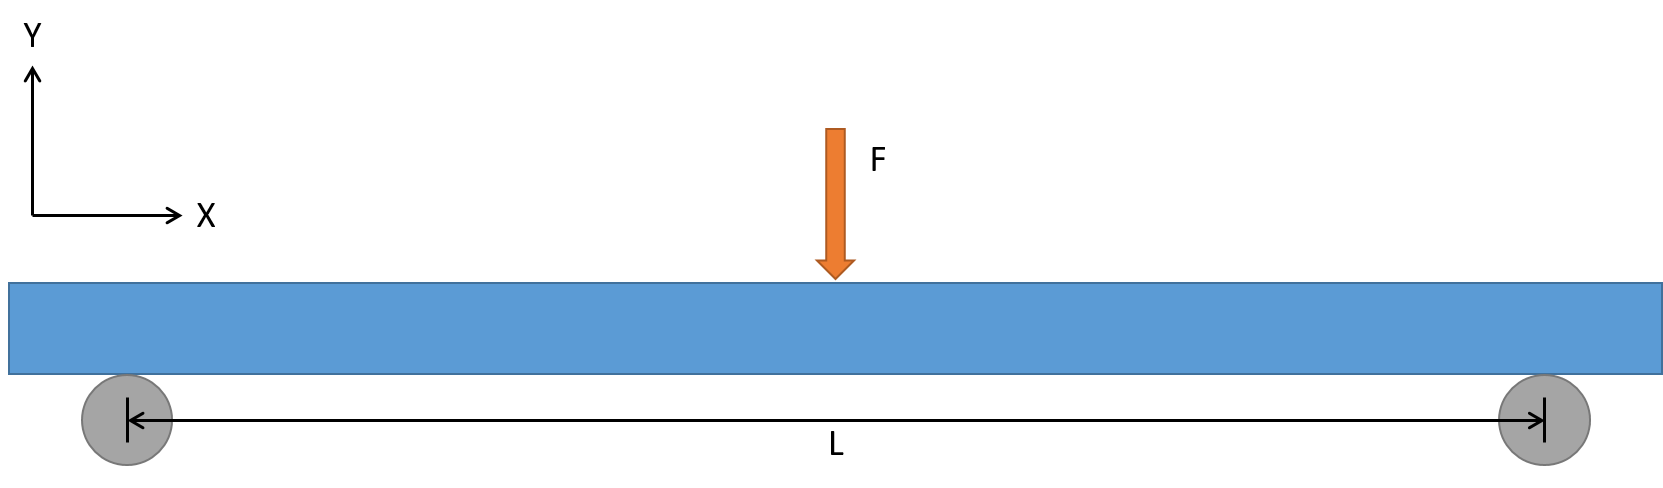
\includegraphics[width=\textwidth]{3_Point_Bend}
	\label{fig:3_Point_Bend}
\end{figure}



\begin{figure} [H]
\centering
	\caption{\label{ref_label_overall}3-Point Bend Fixture}
	\subfloat[Clamp without Bolts]{\label{fig:fixture_unloaded}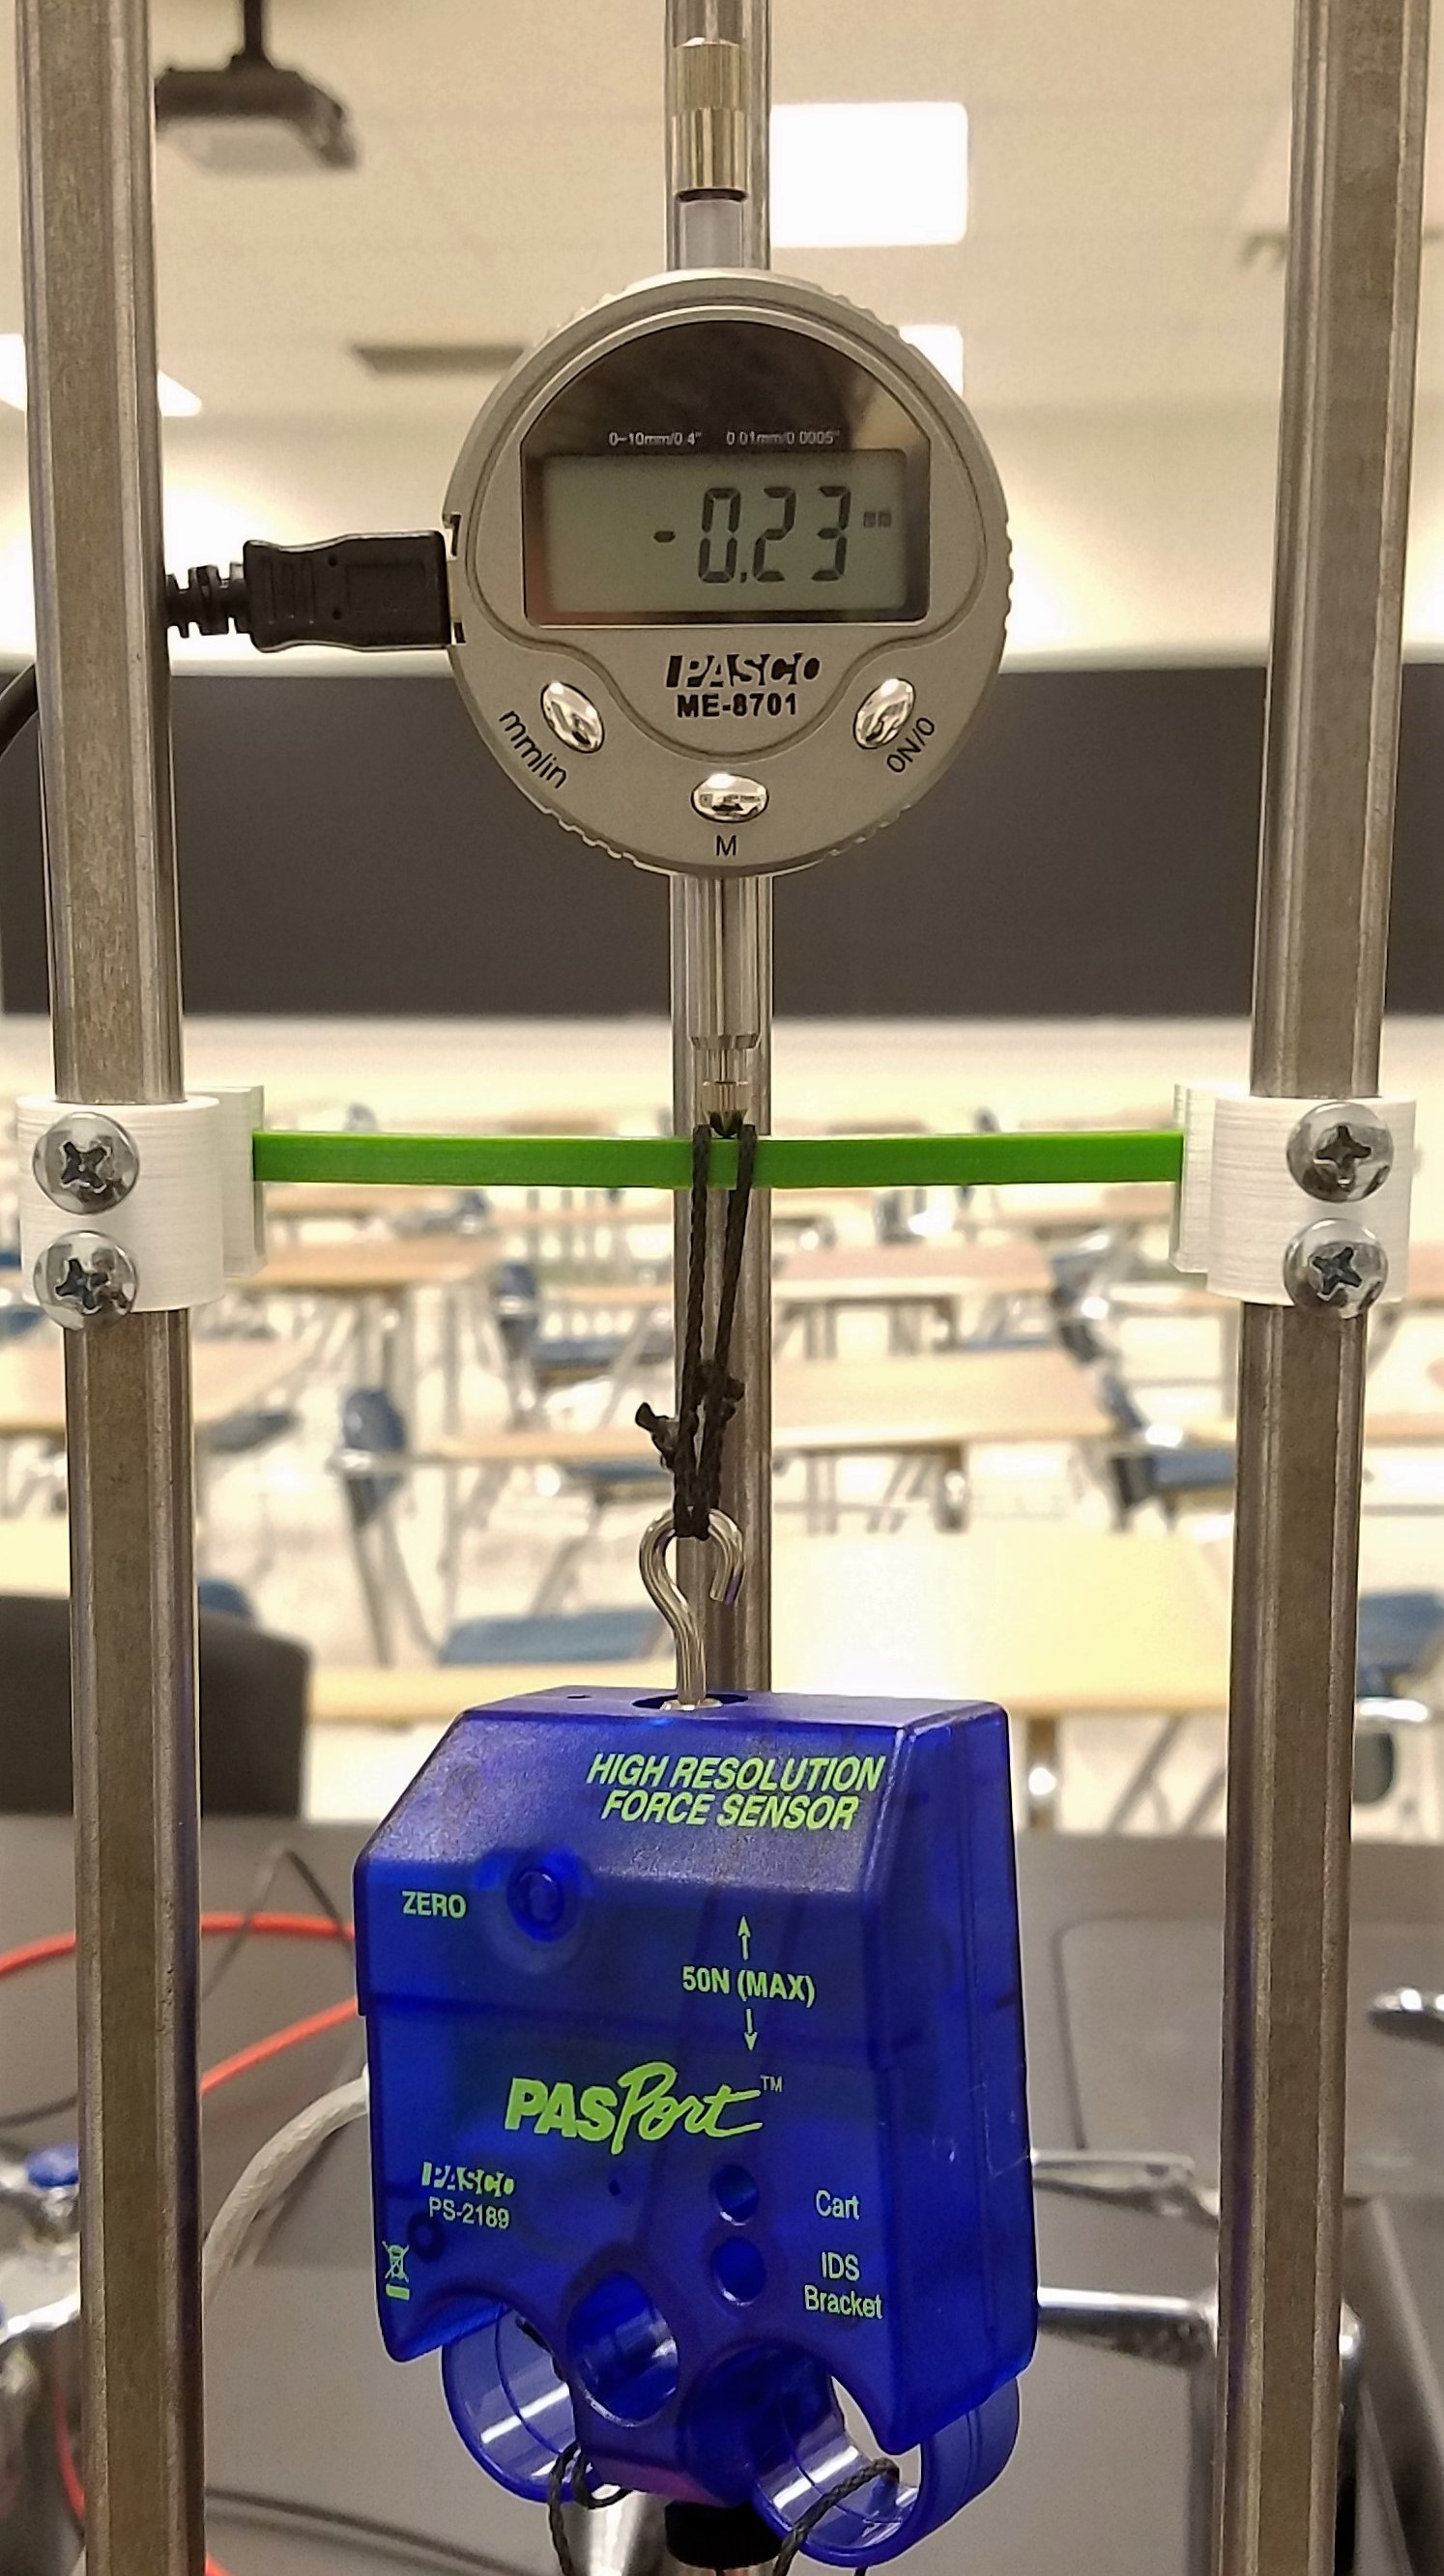
\includegraphics[height=12cm]{FIXTURE_RUNNING_UNLOADED}}\	
	\subfloat[Clamp without Bolts]{\label{fig:fixture_loaded}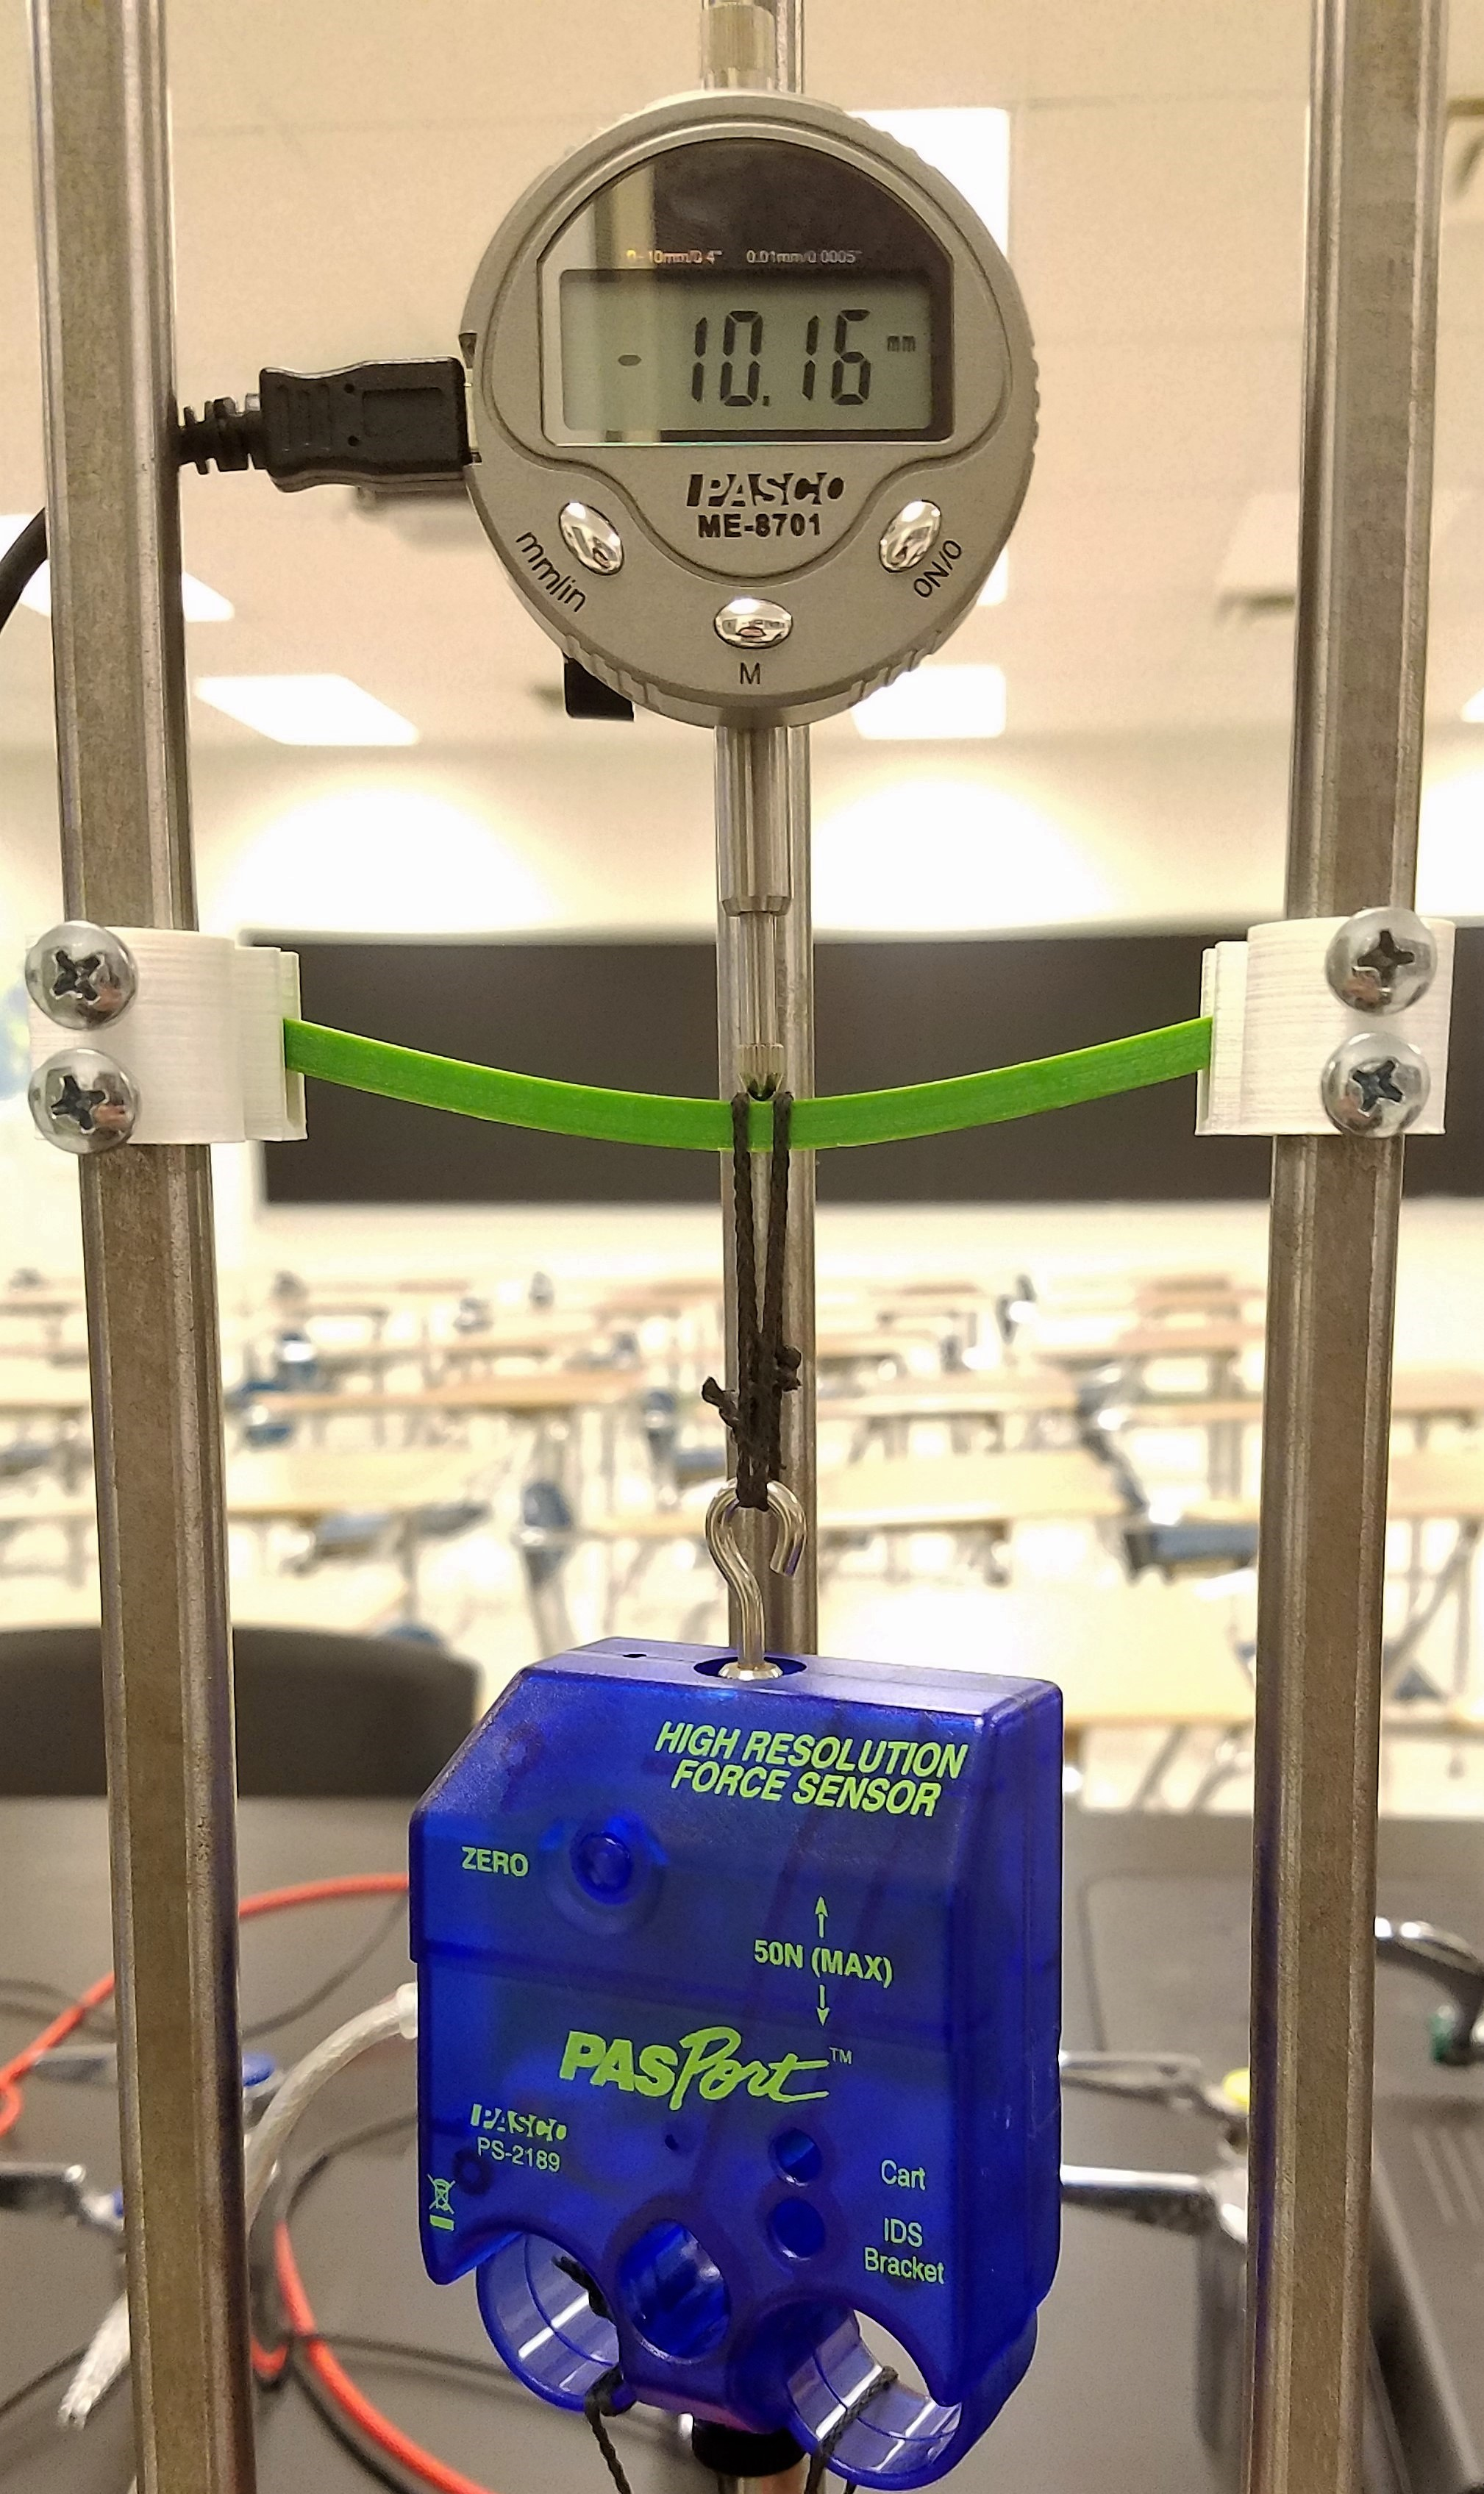
\includegraphics[height=12cm]{FIXTURE_RUNNING_LOADED}}\
\end{figure}

\section{Flexural Modulus of a Beam} \label{sec:modulus}
	With the test fixture being used we assume a beam supported by rollers on each side for our bending stress calculations. The equation below, taken from R.C. Hibbeler's book Statics and Mechanics of Materials, specifies the generalized equation for bending. The bending stress is characterized by the distance between supports, $d$, the height $h$, and width $w$ for the square and rectangular beams.

\begin{equation} \label{eq:1}
IE\frac{d^2v}{dx^2} = M(x)\quad \text{\citep{Hibbeler2010}}
\end{equation}

Assuming a beam supported by two rollers -- thus capable of lateral movement -- with a point force focused on the center of the beam, where $L$ is the distance between the two supports and $F$ is the force applied, the behavior of the beam can be described with the following equations.

\begin{equation} \label{eq:2}
IE\frac{d^2v_1}{dx^2} = Fx, \; 0 \leq x \leq \frac{L}{2}
\end{equation}
\begin{equation} \label{eq:3}
IE\frac{d^2v_2}{dx^2} = Fx, \; \frac{L}{2} \leq x \leq L
\end{equation}

Equations \ref{eq:2} \& \ref{eq:3} can then be integrated to obtain the following array of equations.

\begin{table} [h]
	\centering
	\begin{tabularx}{\textwidth}{| X X |}
	\multicolumn{2}{c}{\textbf{Bending Equations}} \\ \hline
	\vbox{\begin{equation} \label{eq:4} IE\frac{d^2v_1}{dx^2} = Fx \end{equation}} & \vbox{\begin{equation} \label{eq:7} IE\frac{d^2v_2}{dx^2} = Fx \end{equation}} \\
	\vbox{\begin{equation} \label{eq:5} IE\frac{dv_1}{dx} = \frac{1}{2}Fx^2 + C_1 \end{equation}} & \vbox{\begin{equation} \label{eq:8} IE\frac{dv_2}{dx} = \frac{1}{2}Fx^2 + C_3 \end{equation}}\\ 
	\vbox{\begin{equation} \label{eq:6} IEv_1 = \frac{1}{6}Fx^3 + C_1x + C_2  \end{equation}} & \vbox{\begin{equation} \label{eq:9} IEv_2 = \frac{1}{6}Fx^3 + C_3x + C_4 \end{equation}}\\ \hline
	\end{tabularx}
	\captionsetup{textformat=empty,labelformat=blank}
	\caption{Table of Bending Equations}
	\label{tab:bending}
\end{table}
\par

The following boundary conditions are assumed based on the behavior of the beam being supported on rollers at either end and having a point force applied in the center of the beam. Conditions \ref{bc:1} and \ref{bc:2} are assumed because the end points are constricted from vertical movement in the negative Y direction due to the rollers. shown by figure \ref{fig:3_Point_Bend}. The conditions \ref{bc:3} and \ref{bc:4} at $\frac{L}{2}$ are assumed because the deflection and rate of deflection are being measured at the same point from both ends.

\begin{table} [h]
	\centering
	\begin{tabularx}{\textwidth}{ | X  X | }
	\multicolumn{2}{c}{\textbf{Boundary Conditions}} \\ \hline
	\vbox{\begin{equation} \label{bc:1} v_1(0) = 0 \end{equation}} & \vbox{\begin{equation} \label{bc:2} v_2(L) = 0 \end{equation}} \\
	\vbox{\begin{equation} \label{bc:3} v_1\left(\frac{L}{2}\right) = v_1\left(\frac{L}{2}\right) \end{equation}} & \vbox{\begin{equation} \label{bc:4} \frac{dv_1}{dx}\vert_{\frac{L}{2}} = \frac{dv_1}{dx}\vert_{\frac{L}{2}} \end{equation}} \\ \hline
	\end{tabularx}
	\captionsetup{textformat=empty,labelformat=blank}
	\caption{Table of Boundary Conditions}
	\label{tab:bounds}
\end{table}
\par


While the boundary conditions can be applied to the equations in any order, for simplicity one start by applying boundary condition \eqref{bc:1} to \eqref{eq:6} to solve for $C_2$ and find that $C_2 = 0$. \eqref{eq:5} and \eqref{eq:8} can then be evaluated using boundary condition \eqref{bc:4} to determine $C_1 = C_3$ as shown below.

\begin{align*}
v_1(0) = 0; & \quad \frac{1}{6}F\cdot0 + C_1\cdot0 + C_2 = 0 \; \implies \; C_2 = 0 \\
\frac{dv_1}{dx}\vert_{\frac{L}{2}} = \frac{dv_1}{dx}\vert_{\frac{L}{2}}; & \quad \frac{F}{2}\left(\frac{L}{2}\right)^2 + C_1 = \frac{F}{2}\left(\frac{L}{2}\right)^2 + C_3 \; \implies \; C_1 = C_3 \\
\end{align*}

Following this, evaluating \eqref{eq:6} and \eqref{eq:9} with the boundary condition \eqref{bc:3} further simplifies the set of equations by showing that $C_4 = 0$.

\begin{align*}
v_1\left(\frac{L}{2}\right) = v_1\left(\frac{L}{2}\right); & \quad  \frac{F}{6}\left(\frac{L}{2}\right)^3 + \frac{C_1L}{2} = \frac{F}{6}\left(\frac{L}{2}\right)^3 + \frac{C_1L}{2} + C_4 \; \implies \; C_4 = 0
\end{align*}

Finally, one can apply the boundary condition \eqref{bc:2} to \eqref{eq:9}.

\begin{align*}
v_2 = 0; & \quad \frac{FL^3}{6} + C_1L = 0 \; \implies \; C_1 = -\frac{FL^2}{6}
\end{align*}

By applying these solutions, equations \eqref{eq:6} and \eqref{eq:9} become the following:

\begin{align*}
v_1(x) = \frac{F}{6IE}(x^3 - L^2x) = v_2
\end{align*}

Now, one can conclude that $v_1 = v_2$ and simply use the following equation to determine the displacement of a beam in a 3-point bend fixture.

\begin{equation} \label{eq:10}
v(x) = \frac{F}{6IE}(x^3 - L^2x)
\end{equation}

Because a symmetrical bending experiment is being performed with a point load centered directly at $\frac{L}{2}$, this equation can be evaluated at the midpoint to come up with a solution for a three point bend test consisting of a beam on two rollers and a force applied at the center.

\begin{align}
v\left(\frac{L}{2}\right) = \frac{F}{6IE}\left[\left(\frac{L}{2}\right)^3 - \frac{L^3}{2}\right] \nonumber \\
v\left(\frac{L}{2}\right) = \frac{F}{6IE}\left[\frac{L^3}{8} - \frac{L^3}{2}\right] \nonumber \\
\label{eq:v} v\left(\frac{L}{2}\right) = \frac{FL^3}{48IE}
\end{align}

Knowing this, and substituting in $I = \frac{1}{12}bh^3$ we can rearrange our formula for finding the modulus of elasticity as long as our bend point stays centered.

\begin{equation}\label{eq:modulus}
E(F,L,b,h,v) = \frac{FL^3}{4vbh^3}
\end{equation}
Equation \eqref{eq:modulus} will be used in calculations for determining the modulus of elasticity of PLA and ABS square and rectangular beams using experimental data collected. The method of data collection and test setup will be explained in chapter 4. The table below outlines each of the variables significance and how they will be measured.

\begin{table} [h]
	\centering
	\begin{tabularx}{\textwidth}{ l | l | X}
		\multicolumn{3}{c}{\textbf{\eqref{eq:modulus}Variable Descriptions}} \\ \hline
		E & Modulus of Elasticity & Calculated using \eqref{eq:modulus}\\
		L & Distance between beam supports & Measured using calipers.\\
		b & Base of beam cross section & Measured using calipers. \\
		h & Height of beam cross section & Measured using calipers.\\
		F & Force applied & Measured using PASCO force sensor. \\
		v & Displacement & Measured using PASCO displacement gauge. \\
	\end{tabularx}
	\label{tab:variables}
	\captionsetup{textformat=empty,labelformat=blank}
	\caption{Table of Variables for \eqref{eq:modulus}}
\end{table}
\par
The length of the beams will remain constant based on the test fixture. The width and height of the beams were measured at both end points and midpoint and then averaged to obtain the figures that were used in calculations of the elastic modulus. The beam measurements are included in Appendices \ref{app:square} and \ref{app:rectangle}.

\section{Square and Rectangular Beam Uncertainty}
The uncertainty of estimating the behavior of a beam was calculated according to equation \ref{eq:sq_rect_uncertainty}. The uncertainty in predicting the behavior of the Square and Rectangular beams is important to observe and record as it provides insight as to how one would design a structure and the variance in strength that would be expected. $F_{Predicted}$ is defined as the force calculated to bend the beam to a randomly chosen deflection within the linear elastic region. $F_{Actual}$ is the actual force that applied to bend the beam to that deflection amount during experimentation.

\begin{equation}\label{eq:sq_rect_uncertainty}
U = 100*\frac{F_{Predicted}-F_{Actual}}{F_{Actual}}
\end{equation}

\section{I-Beam Predictions}
Based on the results for the Modulus of Elasticity of both ABS and PLA specimens, an Excel spreadsheet was used to determine the moment of inertia and potential strength of a 100\% fill I-beam when given dimensions of the top, web and bottom of the beam. Appendix \ref{app:ibeams}\par
	The beams' predicted deformation is calculated by first finding the moment of inertia of the cross-sectional area of the beam and then inserting it into the following equation from \ref{sec:modulus}. 

\begin{equation}
v = \frac{FL^3}{48IE}
\end{equation}

\section{PLA I-Beam Uncertainty}
The uncertainty of estimating the behavior of the I-beams was calculated according to equation \ref{eq:ib_uncertainty}. $v_{Predicted}$ is the amount of deflection that one would expect to see when applying a 40N load to the midpoint of the beam and $v_{Actual}$ is the observed deflection when 40N is applied.

\begin{equation}\label{eq:ib_uncertainty}
U = 100*\frac{v_{Predicted}-v_{Actual}}{v_{Actual}}
\end{equation}
\chapter{Tests Performed, Results and Discussion} \label{chap:tests}
\section{Phase I: Determining Moduli of Elasticity}
\subsection{Bending Tests}
\begin{figure} [H]
\centering
	\caption{Test Fixture and Software}
	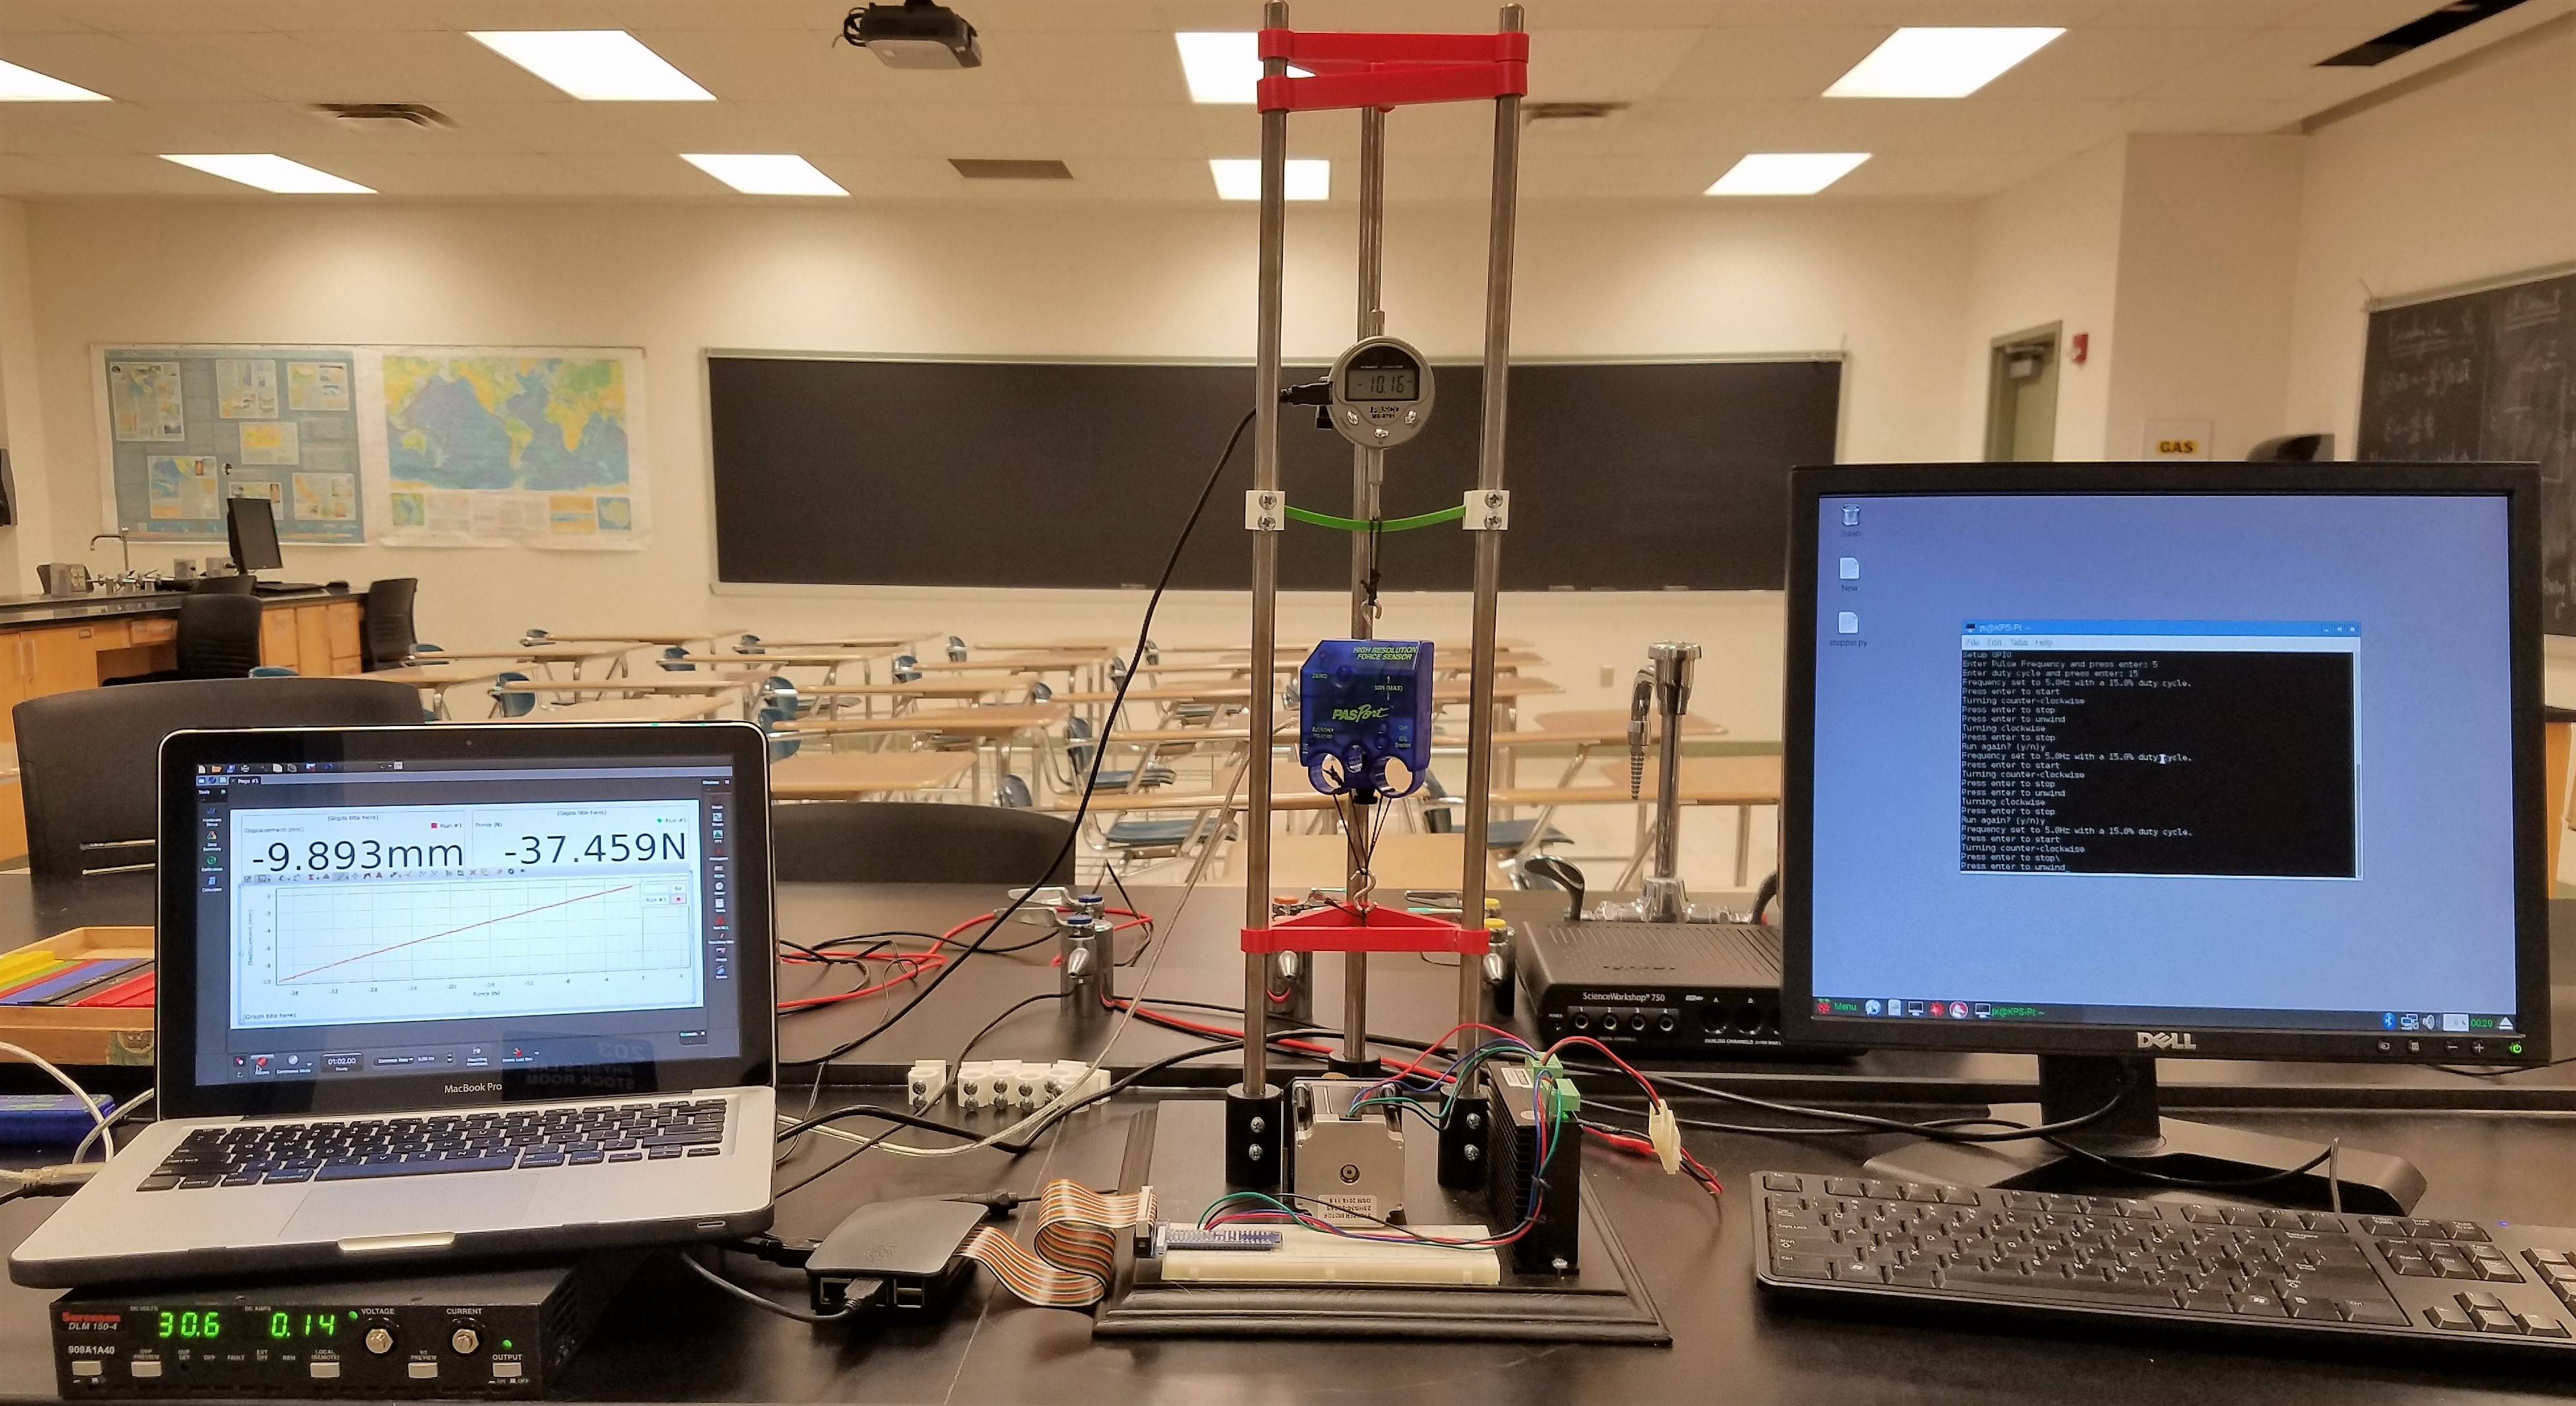
\includegraphics[width=\textwidth]{FIXTURE_SETUP_WHOLE}
	\label{fig:test_fixture}
\end{figure}

All bending tests were conducted using a custom built test fixture. The length of the section to be bent was kept at $120 +0.23/-.033 mm$ for all specimens using a set of custom designed collars (the red components shown in \ref{fig:test_fixture}) to keep the test fixture oriented properly. A NEMA 23 CNC bi-directional stepper motor, model 23HS30-2804S, was used and controlled using a M542T high resolution stepper motor controller at a 1.8\degree step. The motor controller was powered with a Sorensen DLM150-4 power supply at 30V and a maximum of 0.4A and the stepping was controlled using PWM outputs from a Raspberry PI microcomputer (code is attached in Appendix A) at a rate of 5 Hz with a 15\% duty cycle. Non-elongating woven kevlar cord was used to perform the bending tests in order to minimize error caused by deformation of the mechanisms used to apply loading to the test specimen. \par

	PASCO Capstone software was used to record data captured by the PASCO High Resolution Force Sensor (PS-2189) and PASCO Displacement Sensor (PS-2204) at a 5 Hz common rate. The force applied to the specimens started at approximately 1N and was raised to a maximum of 50N, or until a deformation exceeding the measuring capabilities of the deformation gauge was reached.

\subsection{Test Fixture Design}
\begin{figure} [H]
\centering
	\caption{Test Fixture}
	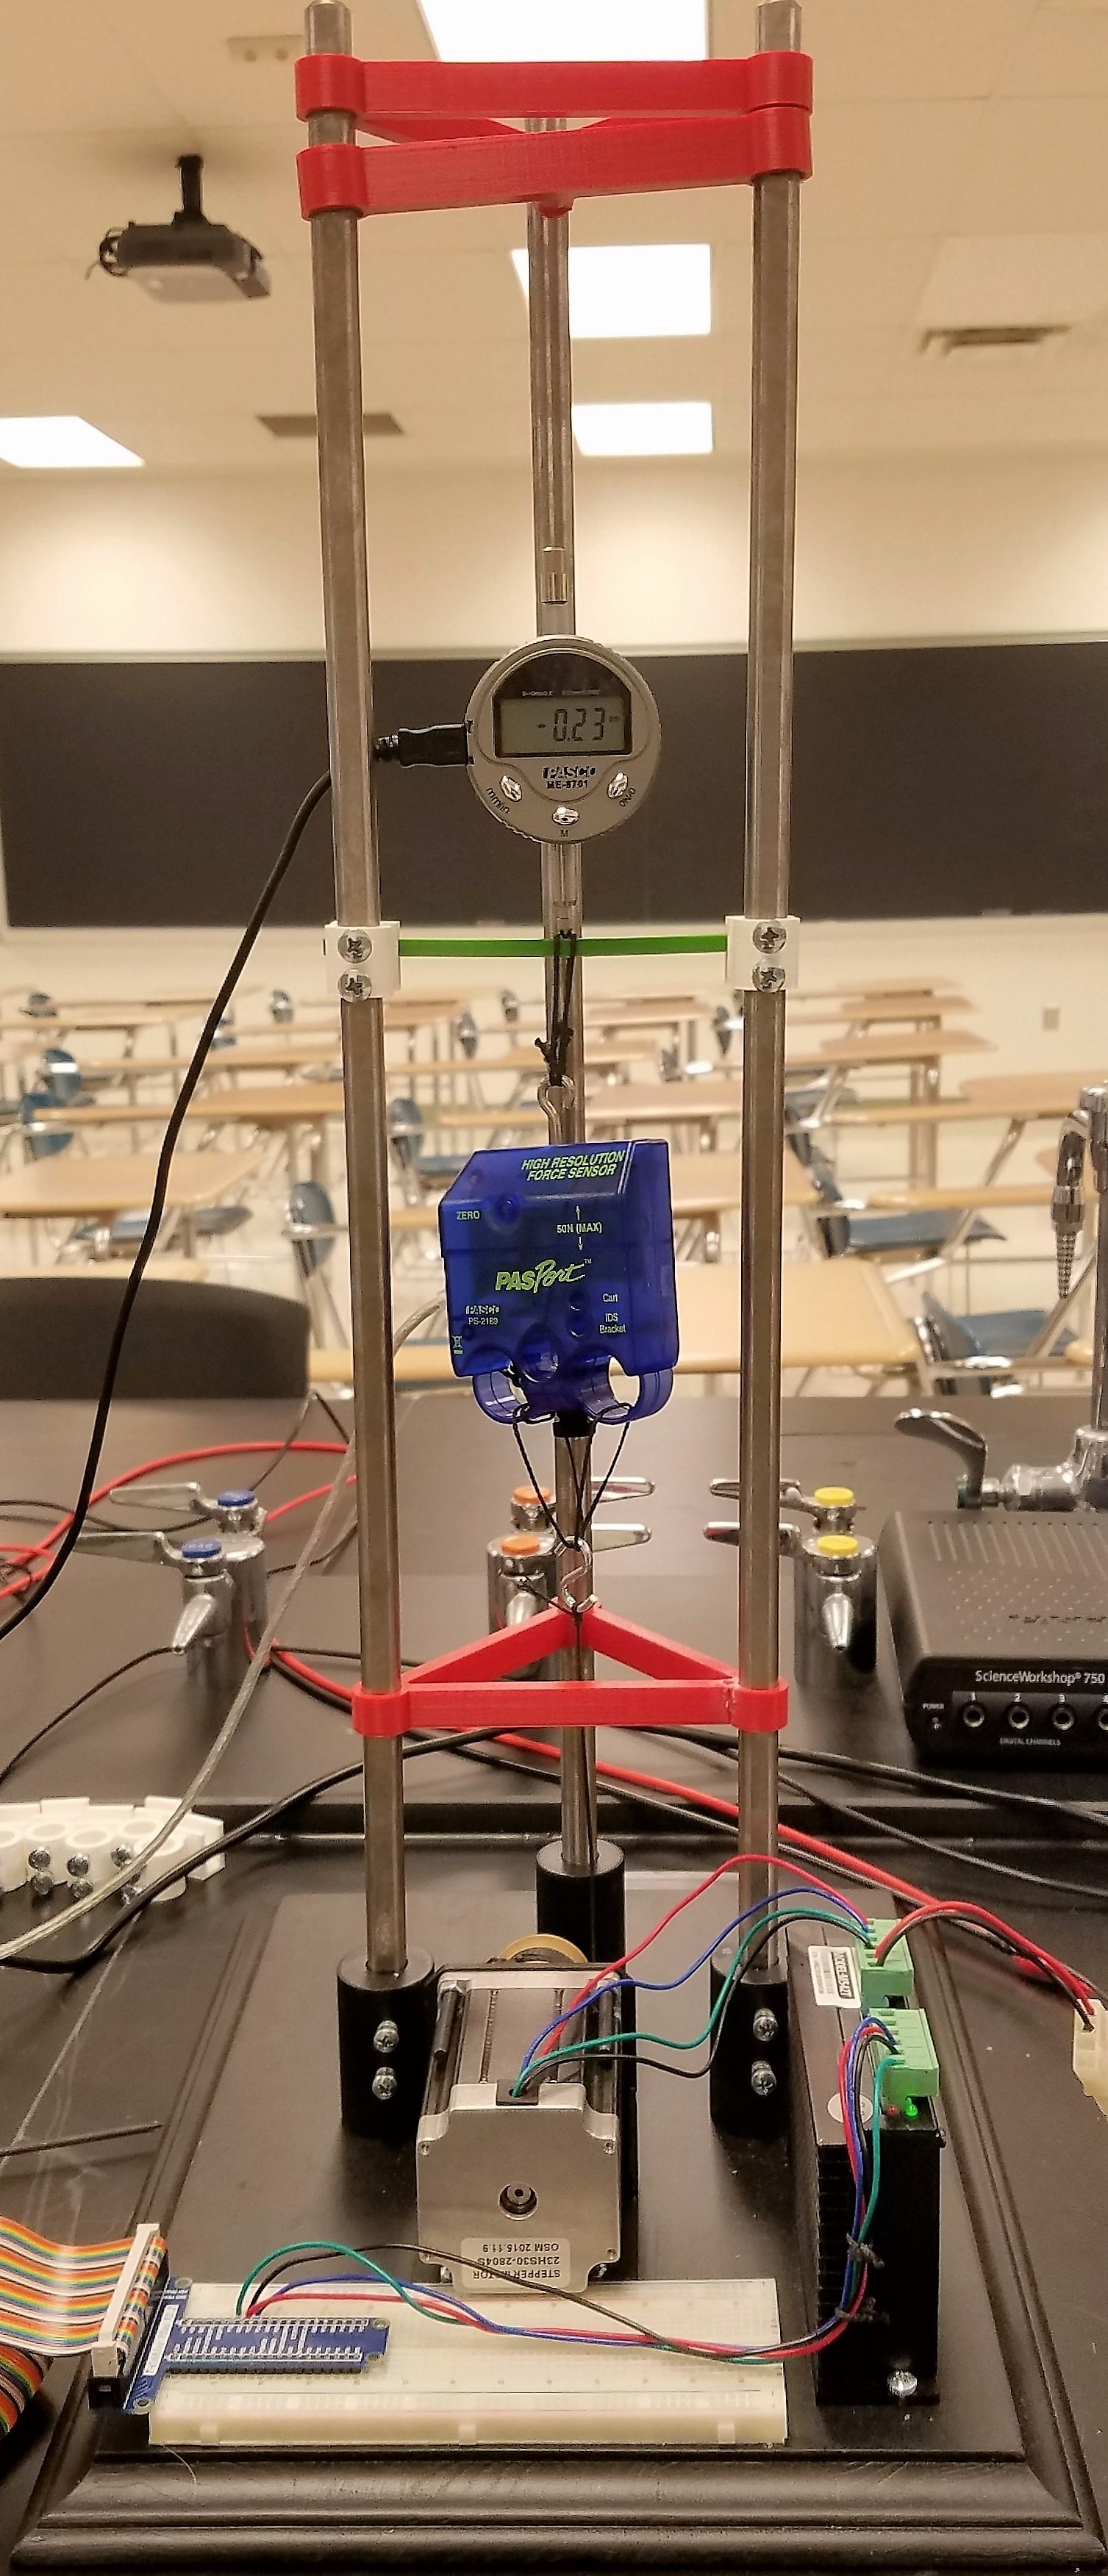
\includegraphics[height=12cm]{FIXTURE_SETUP_DETAIL}
	\label{fig:test_fixture_detail}
\end{figure}

\par
The test fixture in figure \ref{fig:test_fixture_detail} was designed in order to have a bending length $L$ from \ref{eq:modulus} of 120mm. The bending fixtures were created in Solidworks as detailed by the drawing (figure \ref{fig:Bend_Point_Dwg})and were designed to fit the specimens based on measured sizes with minimal tolerance for movement in order to keep the application of force constant throughout the bending tests. Dimension A figure \ref{fig:Bend_Point_Dwg} was set to 5.4mm, 8.2mm, 11.6mm, 15.2mm, to accommodate the different sizes of beams. The center of this bending structure was kept constant in order to provide a bend point 22mm in front of the center of the d-profile rod these fixtures were mounted on. Figure \ref{fig:Bend_Points} shows the printed bend point structures.\par

\begin{figure} [H]
\centering
	\caption{Dimensions of Bend Points}
	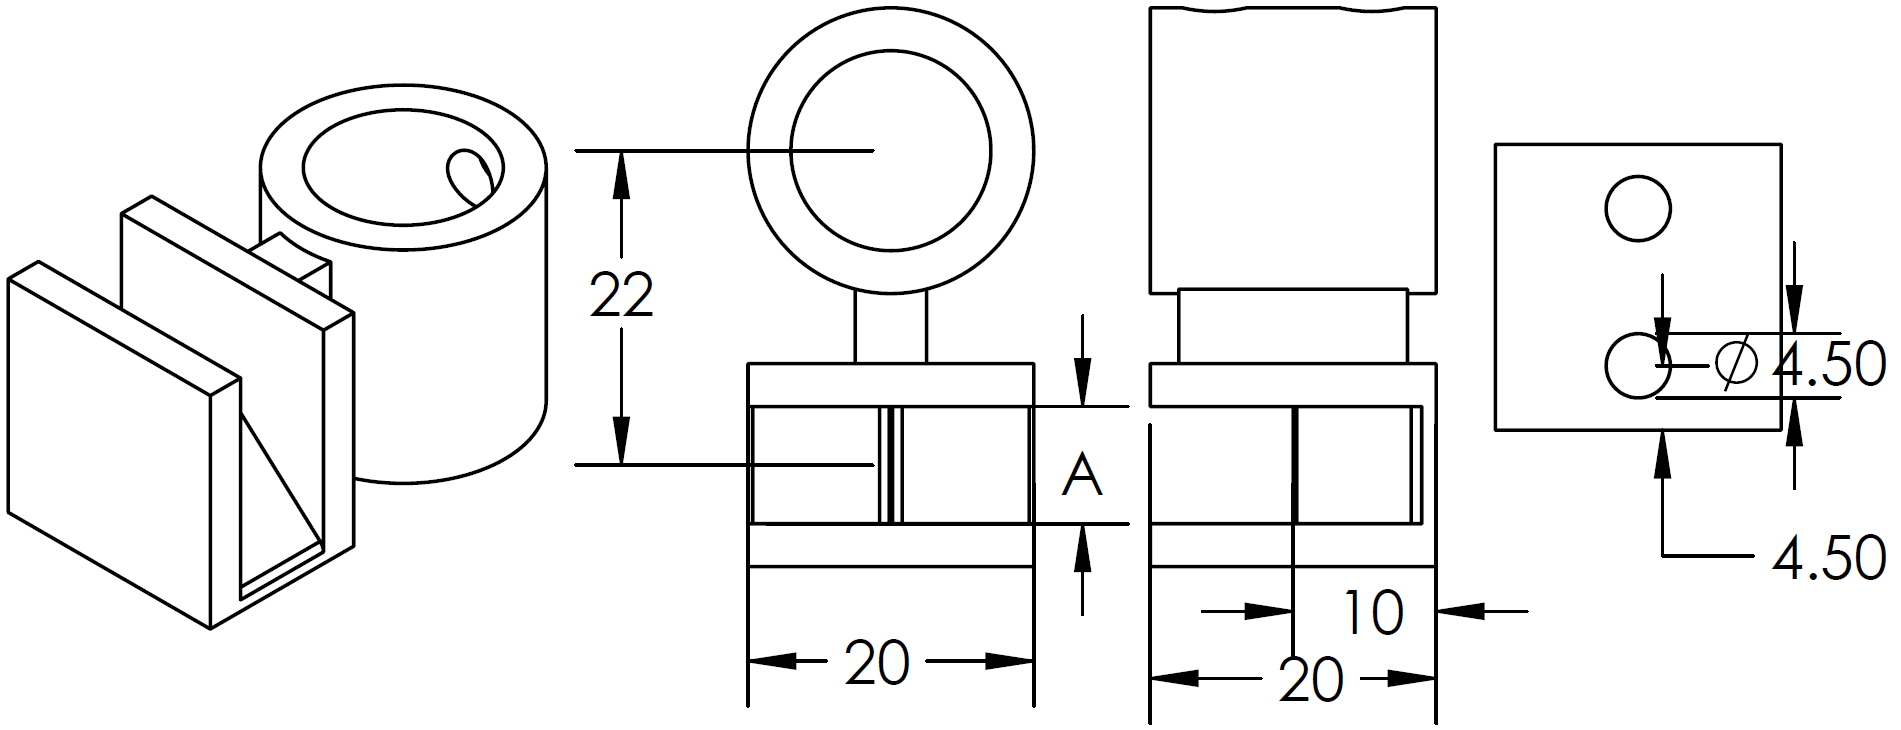
\includegraphics[width=\textwidth]{Bend_Point_DWG}
	\label{fig:Bend_Point_Dwg}
\end{figure}


\begin{figure} [H]
\centering
	\caption{Side View of Fixture Bend Points}
	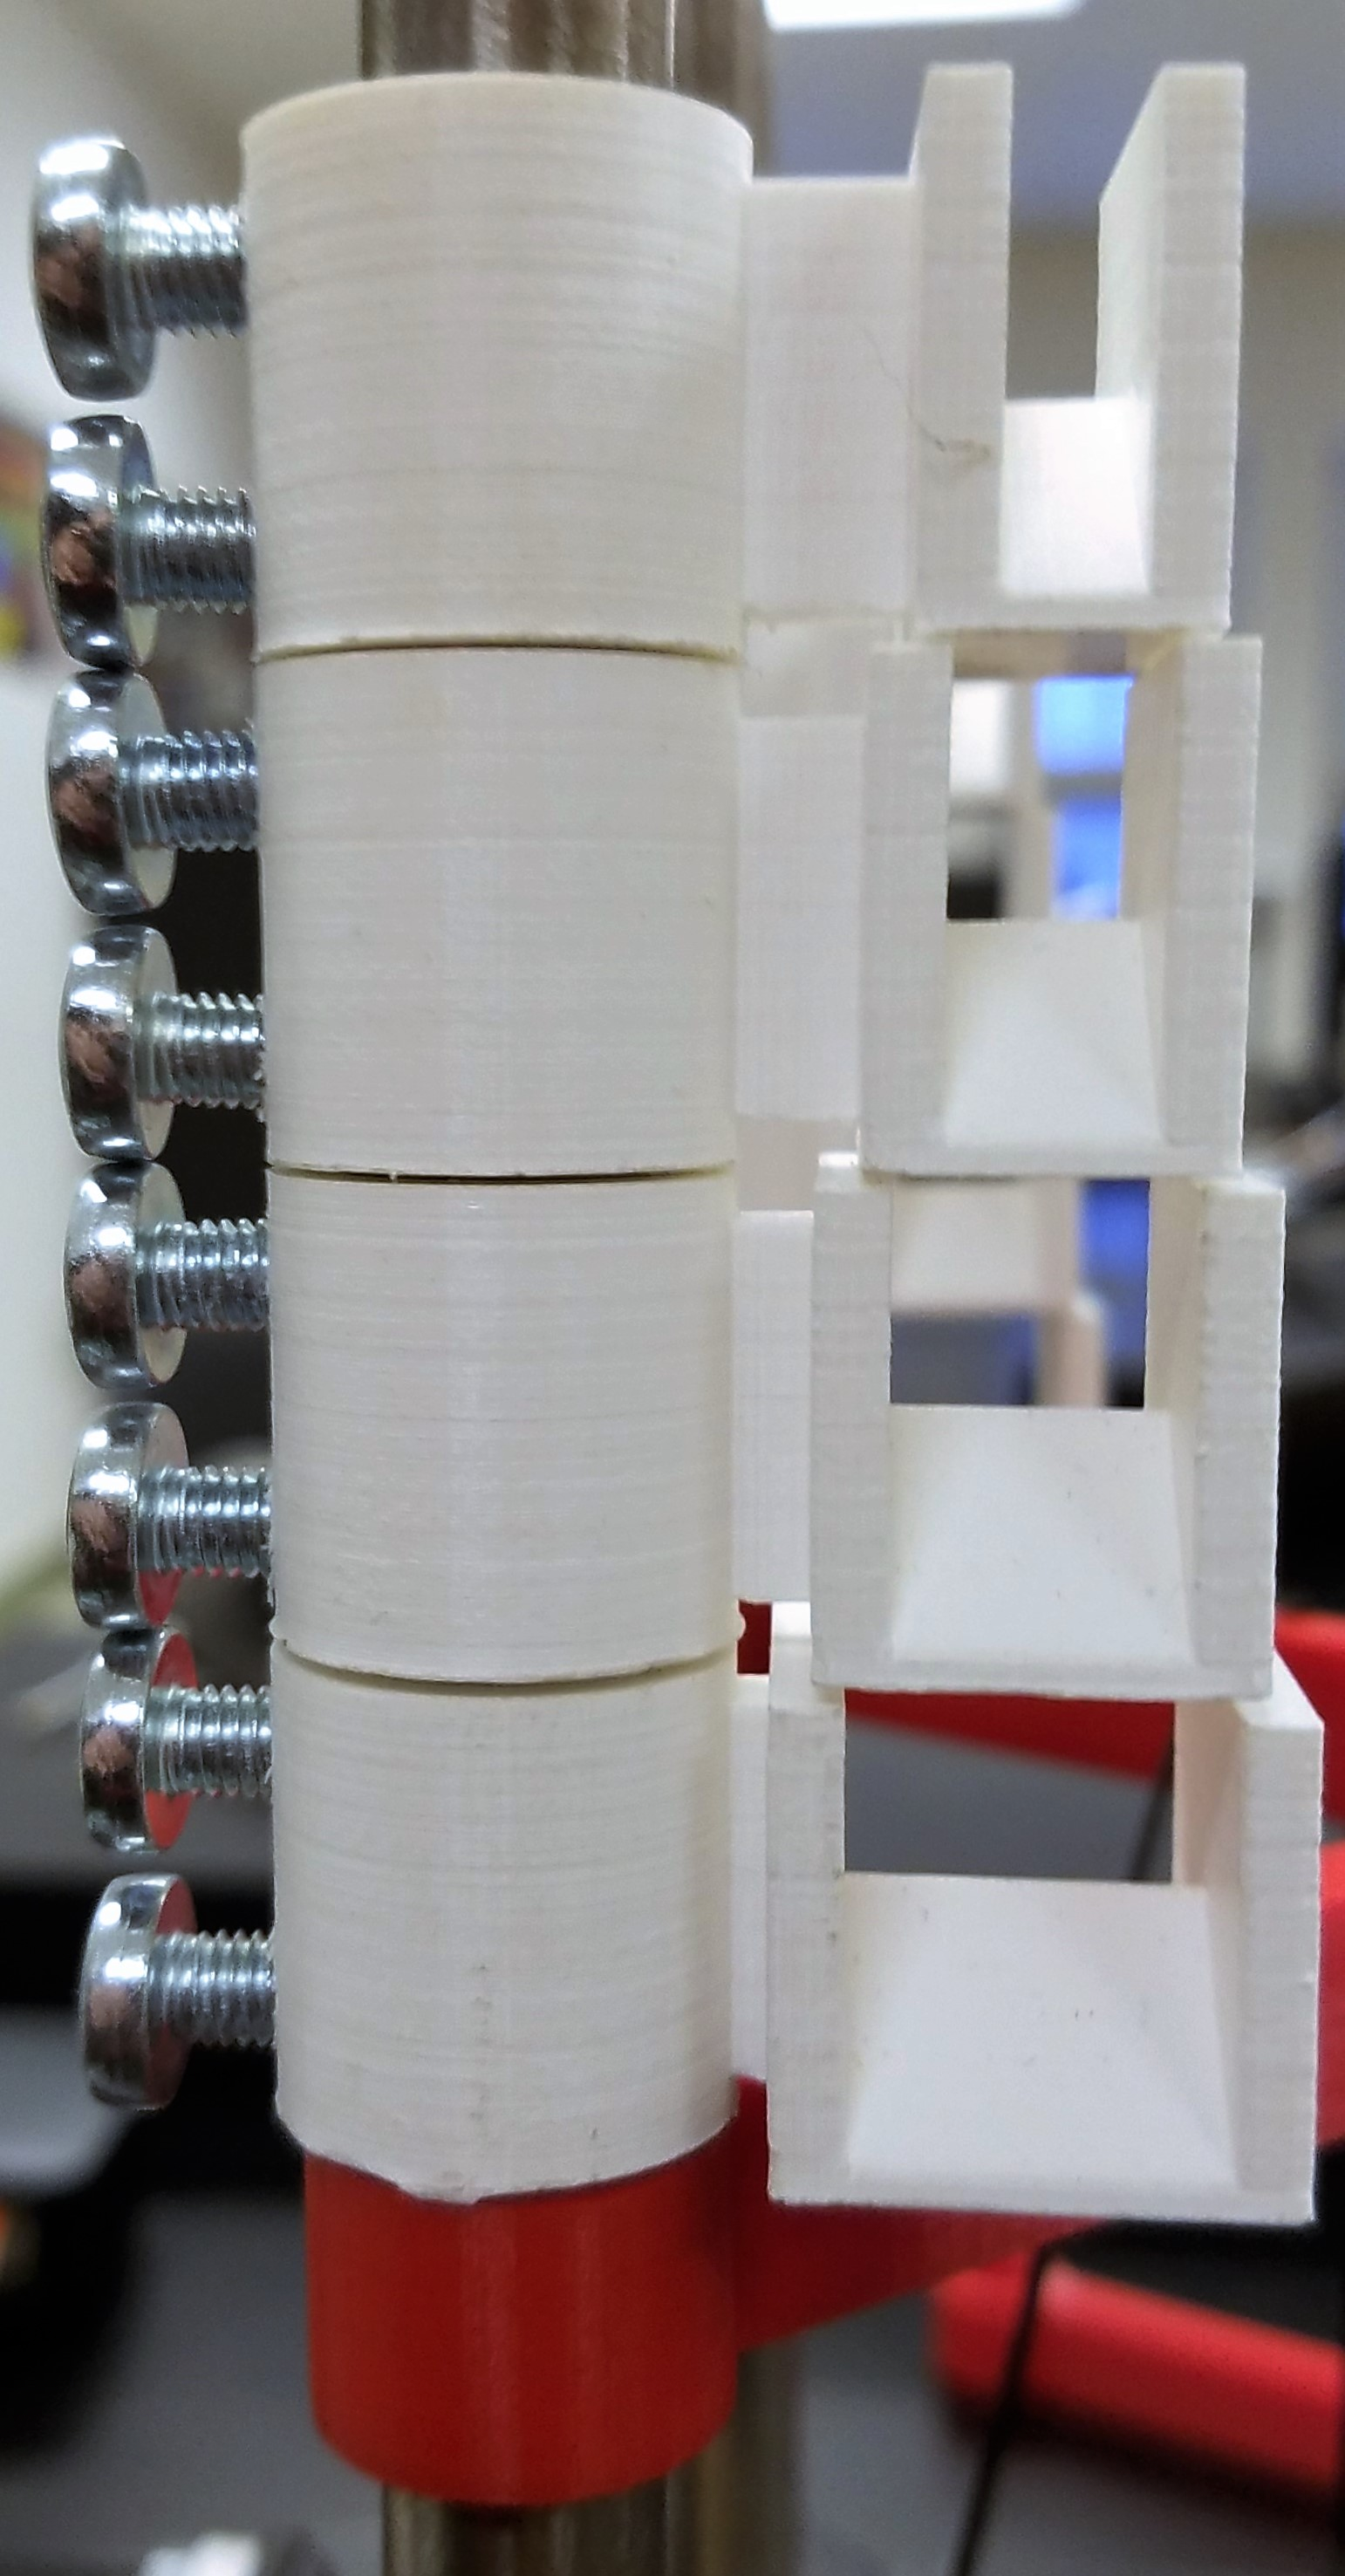
\includegraphics[height=3in]{FIXTURE_SETUP_BEND_POINTS}
	\label{fig:Bend_Points}
\end{figure}

	The test fixtures were designed to be larger and more robust than the beams printed in order to minimize error in measuring the beam deformation by the test fixtures themselves deforming. All test fixtures were printed 100\% solid and then were tapped for a 5mm screw to hold them in place on the test fixture.


\subsection{Test Specimen Design}
	The test specimens for Phase I were designed with two objectives: To determine the effect of increasing density of infill on the 3D printed objects and to see if the size of an object relative to the wall thickness and infill plays any role in determining the strength of the object. An example of 25\% and 50\% infill are shown in figures \ref{fig:25_PLA} and \ref{fig:50_PLA}, respectively. The beams were designed for each rectangular and square size to have identical cross-sectional area. In the table below, the nominal size of the test specimens are listed.
	\begin{table} [H]
		\centering
		\begin{tabular}{ l l l }
		\noalign{\hrule height 2pt}
		Size & Square & Rectangular \\ \hline
		100\% & 5.17x5.17 & 7.53x3.6 \\
		150\% & 7.75x7.75 & 11.3x5.4 \\
		200\% & 10.34x10.34 & 15.06x7.2 \\ \hline
		\multicolumn{3}{c}{Materials} \\ \hline
		ABS & PLA \\ \hline
		\multicolumn{3}{c}{Fill Percentage} \\ \hline
		\multicolumn{3}{c}{20\%} \\
		\multicolumn{3}{c}{50\%} \\
		\multicolumn{3}{c}{100\%} \\ \hline
		\end{tabular}
		\caption{List of Plastic Beam Specimens}
		\label{tab:BeamFab}
	\end{table}

	The measurements for the test specimens were taken at each end and the midpoint of each beam and averaged; this data is available in Appendices B \& C. Table \ref{tab:BeamComp} below shows the average of each set of specimen sizes as well as the deviation from the nominal value. The largest deviation was in the height of the small rectangular samples at 2.78\% deviation from the nominal value listed in Table \ref{tab:BeamFab}.
	
	\begin{figure} [H]
		\centering
		\caption{Printing 25\% Fill PLA Test Specimens}
		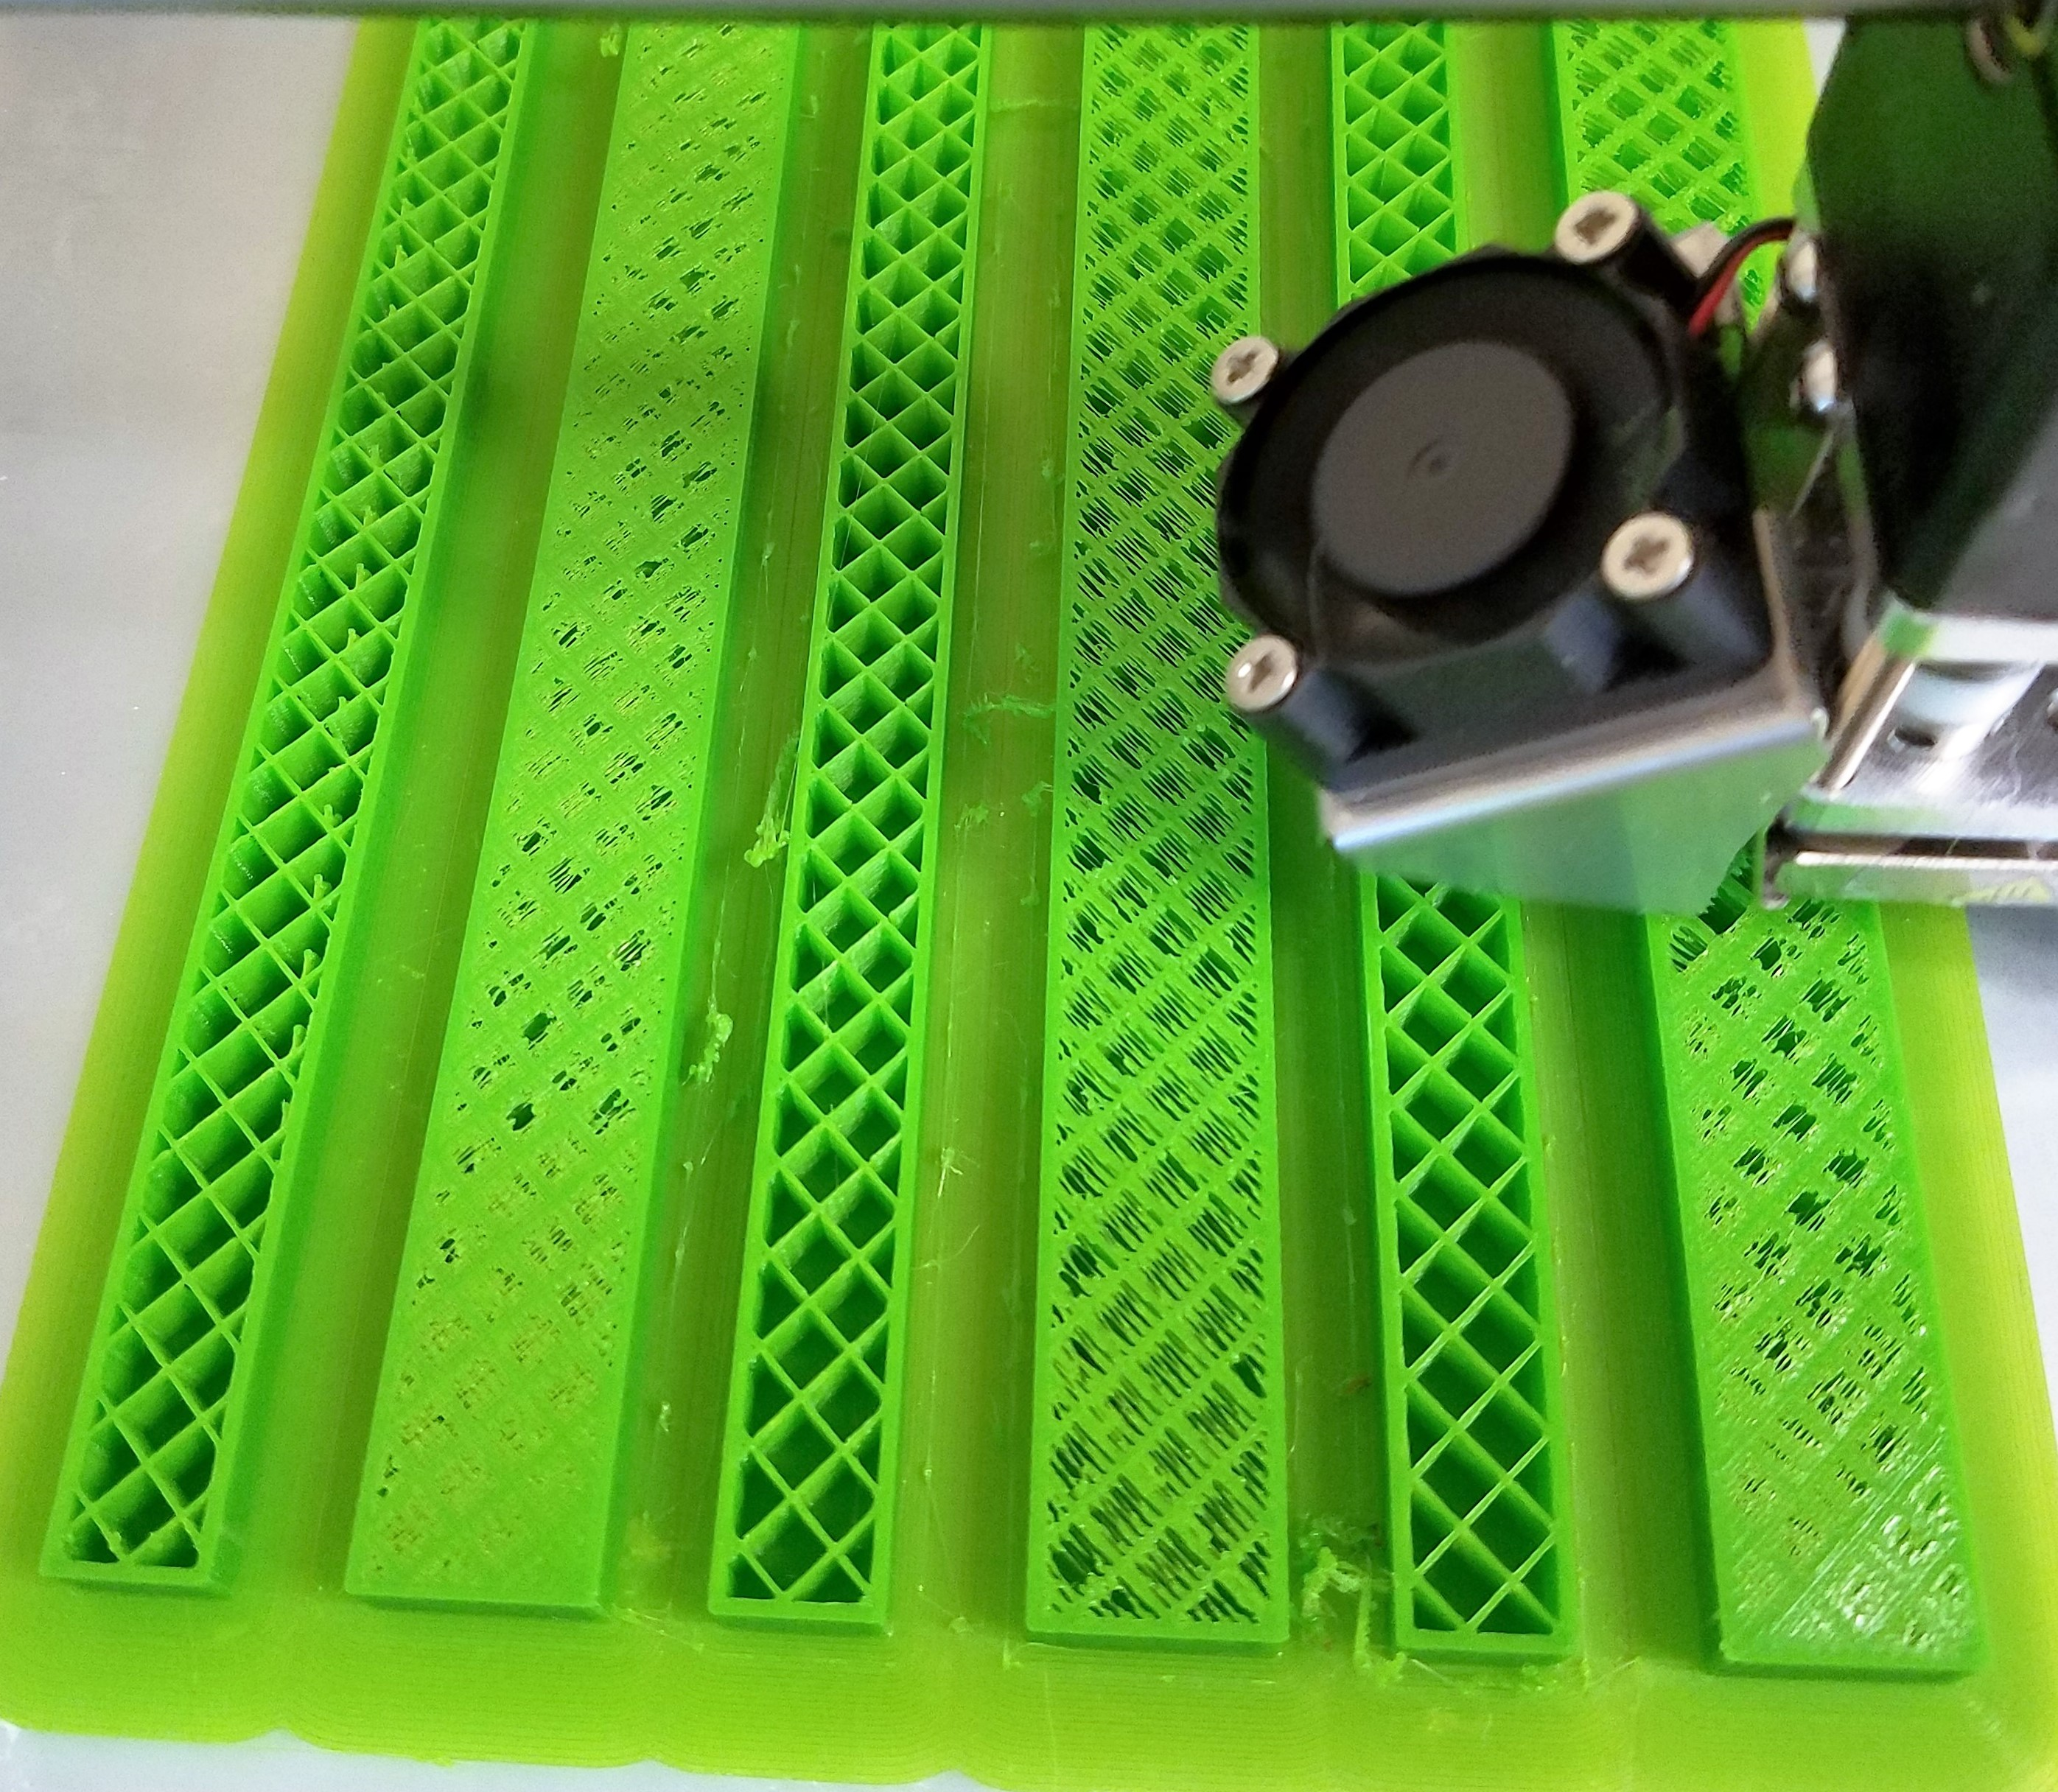
\includegraphics[width=.75\textwidth]{Printer_PLA_Beams_2}
		\label{fig:25_PLA}
	\end{figure}
	
	\begin{table} [h]
		\centering
		\begin{tabularx}{\textwidth}{  X  X  X  X  X  }
		\noalign{\hrule height 2pt}
			& Width (mm) & Height (mm) & Width Deviation (\%) & Height Deviation (\%) \\ \hline
			Square Size 1 & 5.24 & 5.18 & 1.35 & 0.19 \\ 
			Square Size 2 & 7.74 & 7.8 & 0.13 & 0.65 \\ 
			Square Size 3 & 10.25 & 10.34 & 0.87 & 0 \\ \hline
			Rectangle Size 1 & 7.65 & 3.5 & 1.59 & 2.78 \\ 
			Rectangle Size 2 & 11.33 & 5.3 & 0.27 & 1.85 \\ 
			Rectangle Size 3 & 14.98 & 7.12 & 0.53 & 1.11 \\ \hline
		\end{tabularx}
		\caption{List of Plastic Beam Measurements \& Deviation}
		\label{tab:BeamComp}
	\end{table}
	
	\begin{figure} [H]
		\centering
		\caption{Printing 50\% Fill PLA Test Specimens}
		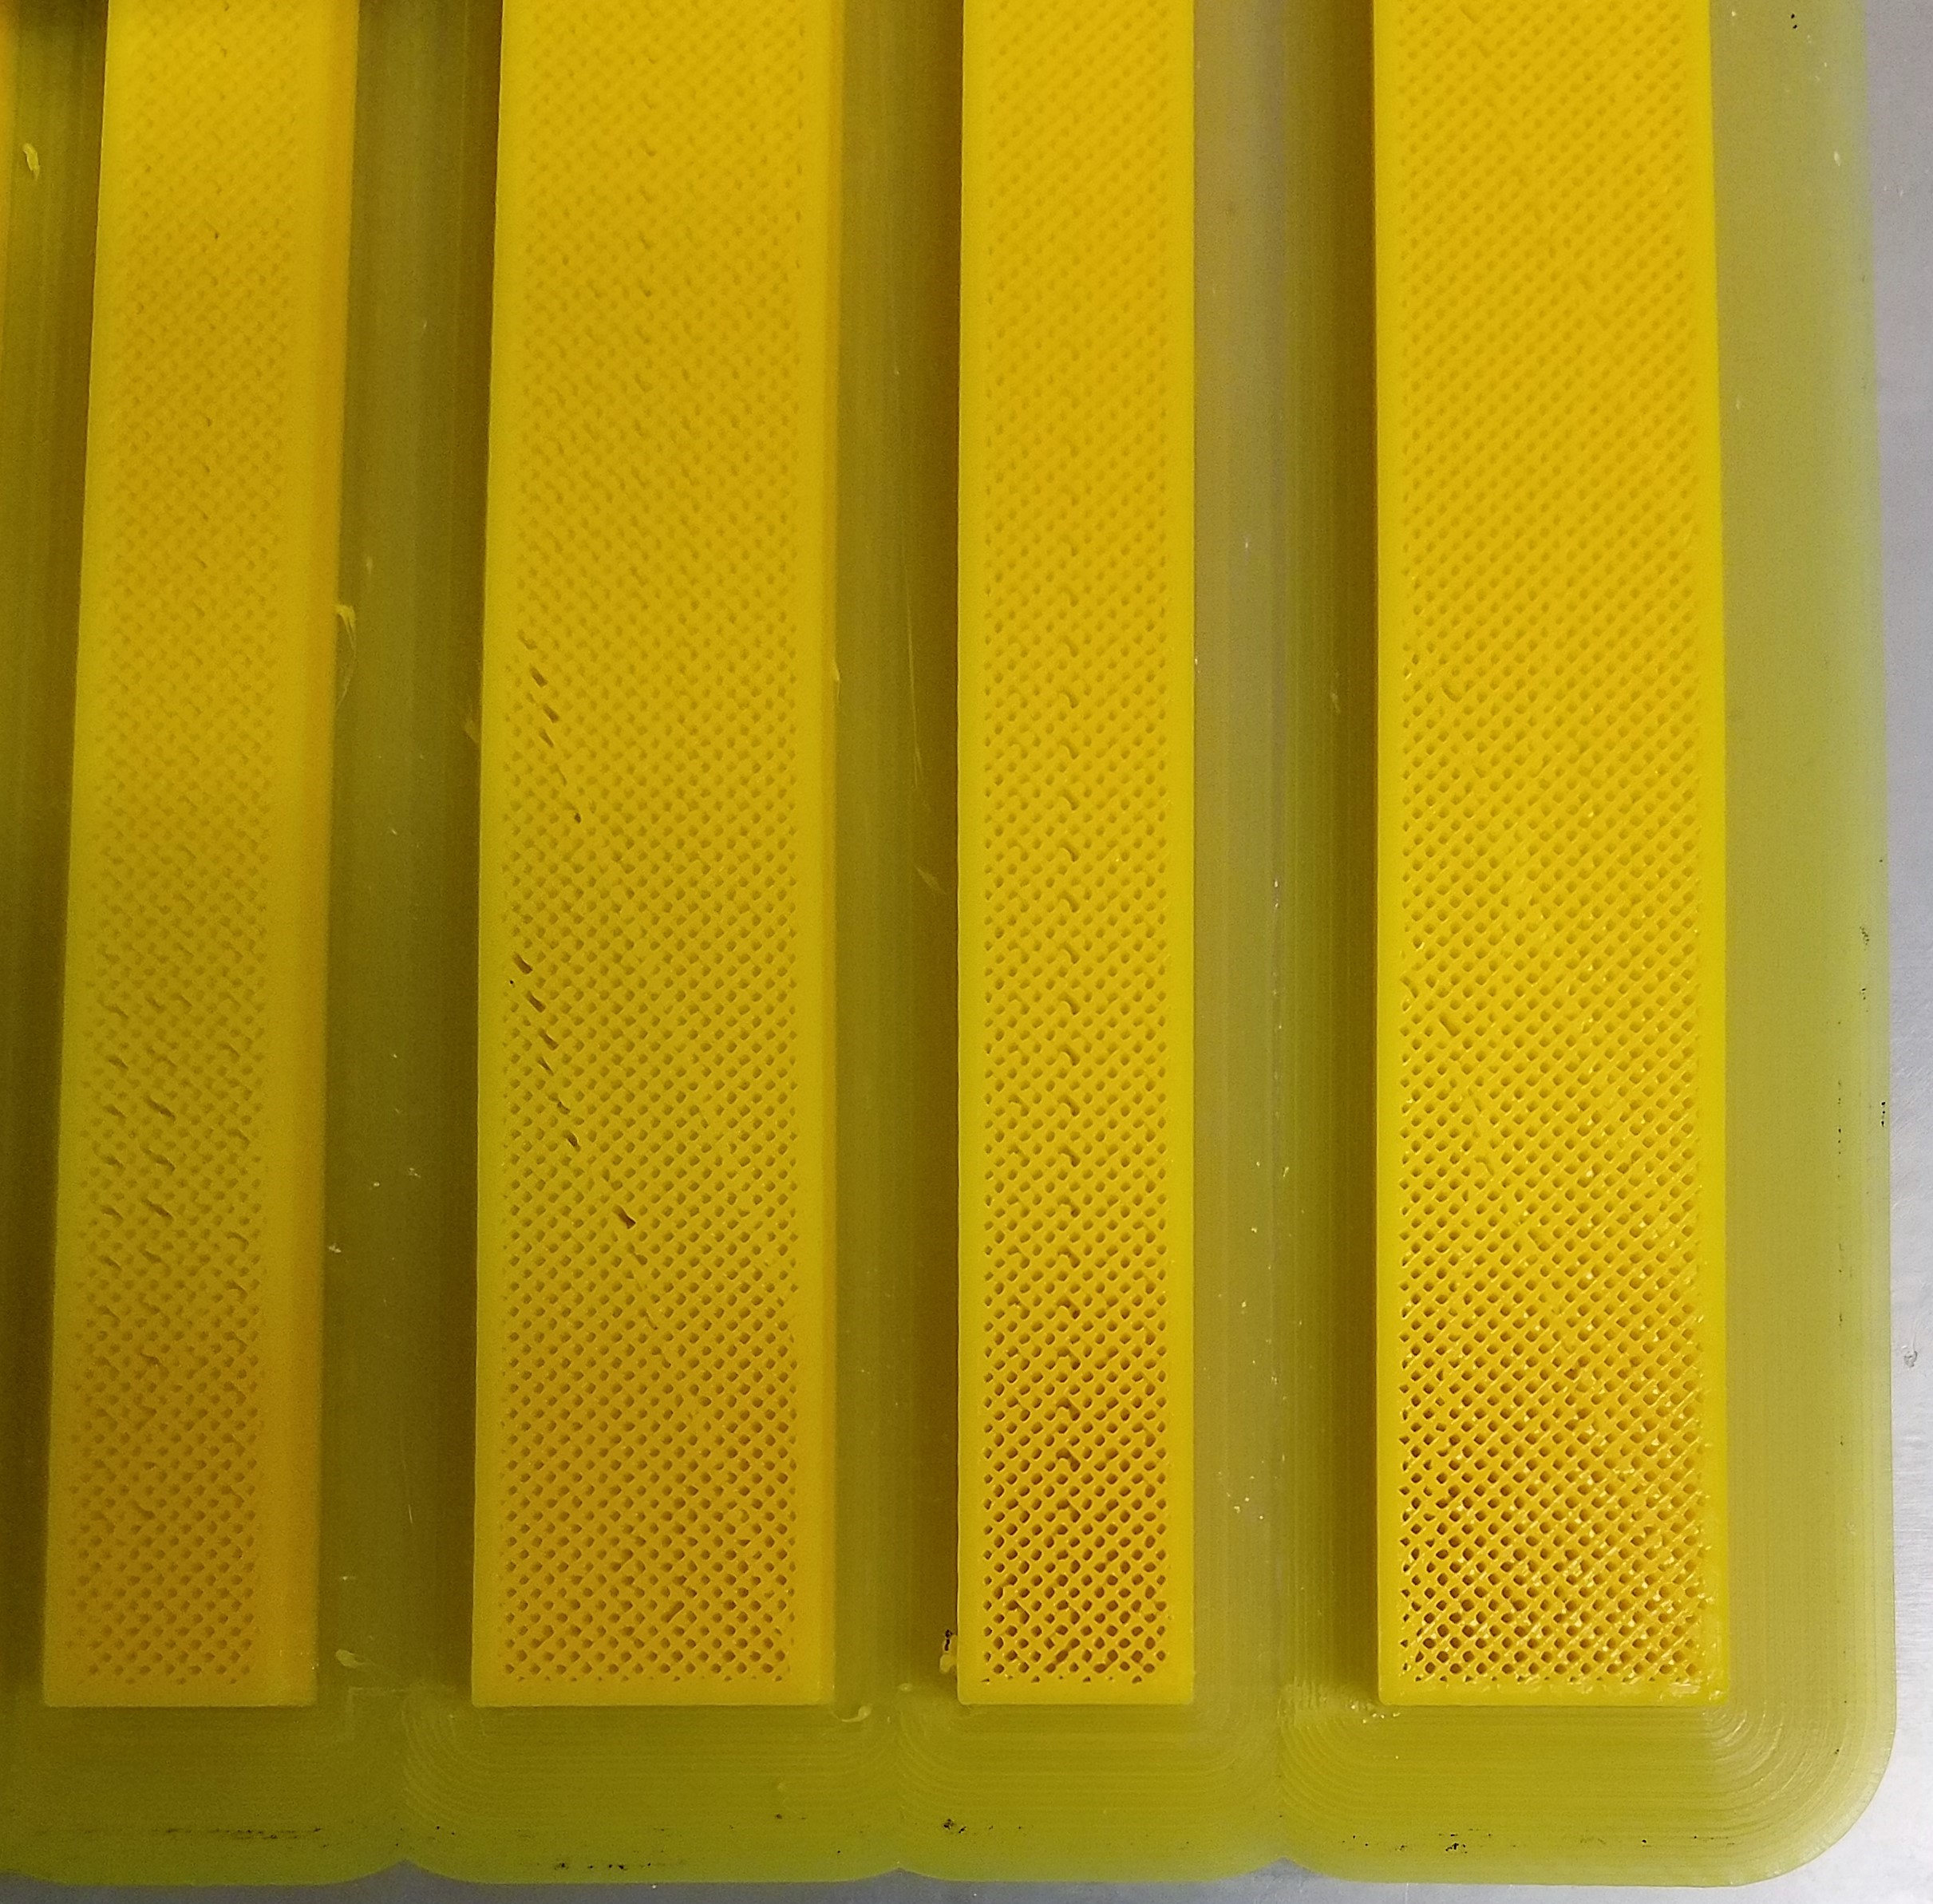
\includegraphics[width=.75\textwidth]{Printer_PLA_Beams_4}
		\label{fig:50_PLA}
	\end{figure}
		
\subsection{Examining Elastic Moduli}
	The Elastic Modulus of each specimen was obtained by using formula \ref{eq:modulus} for each data point and averaging the data for the linear elastic region. From this calculated modulus, an estimated force for deflection within the linear elastic region was determined and then compared to the actual value from experimentation. This uncertainty in the ability to calculate the force at a given deflection, which is similar to the focus of Adamczak, et al., was investigated for all specimens. \citep{Adamczak2014} 
	
	Table \ref{tab:PLAModAvg} details the average of the Modulus of Elasticity and Uncertainty for all 3 samples of each in-fill level of the rectangular and square PLA specimens. The following graphs in figures \ref{fig:PLA_Modulus} \& \ref{fig:PLA_Uncertainty} illustrate the data for the PLA test specimens. Detailed data can be found in appendices B \& C.
	
	\begin{table} [h]
		\centering	
		\begin{tabularx}{\textwidth}{ X X X }
		\noalign{\hrule height 2pt}
			\multicolumn{3}{c}{PLA Modulus of Elasticity Averages} \\ \hline
			SAMPLE & AVG MODULUS (GPa) & UNCERTAINTY (\%) \\ \hline
			SQUARE 25\% & 2.425 & 4.859 \\ 
			SQUARE 50\% & 2.377 & 1.903 \\ 
			SQUARE 100\% & 3.33 & 1.833 \\ 
			RECTANGLE 25\% & 2.419 & 1.712 \\ 
			RECTANGLE 50\% & 2.66 & 1.524 \\ 
			RECTANGLE 100\% & 3.146 & 1.178 \\ \hline
			AVERAGES & 2.726 & 2.168 \\ \hline
		\end{tabularx}
		\caption{Average PLA Beam Specimen Moduli of Elasticity}
		\label{tab:PLAModAvg}
	\end{table}
	
	\begin{figure} [H]
		\centering
		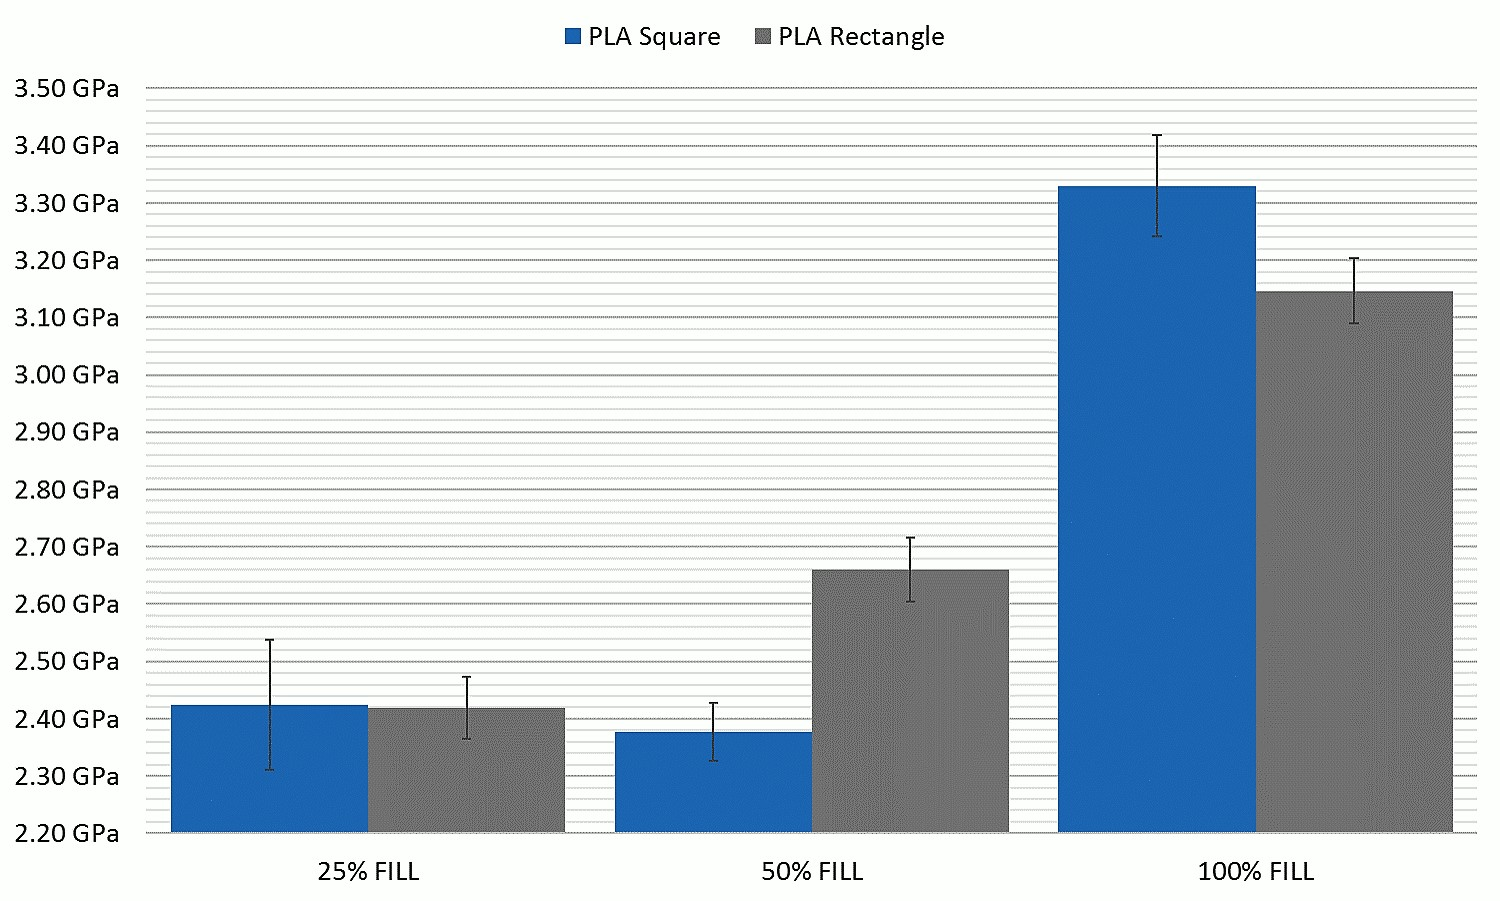
\includegraphics[width=\textwidth]{CHART_PLA_Elasticity}
		\caption{Average PLA Modulus of Elasticity (GPa)}
		\label{fig:PLA_Modulus}
	\end{figure}
	
	\begin{figure} [H]
		\centering
		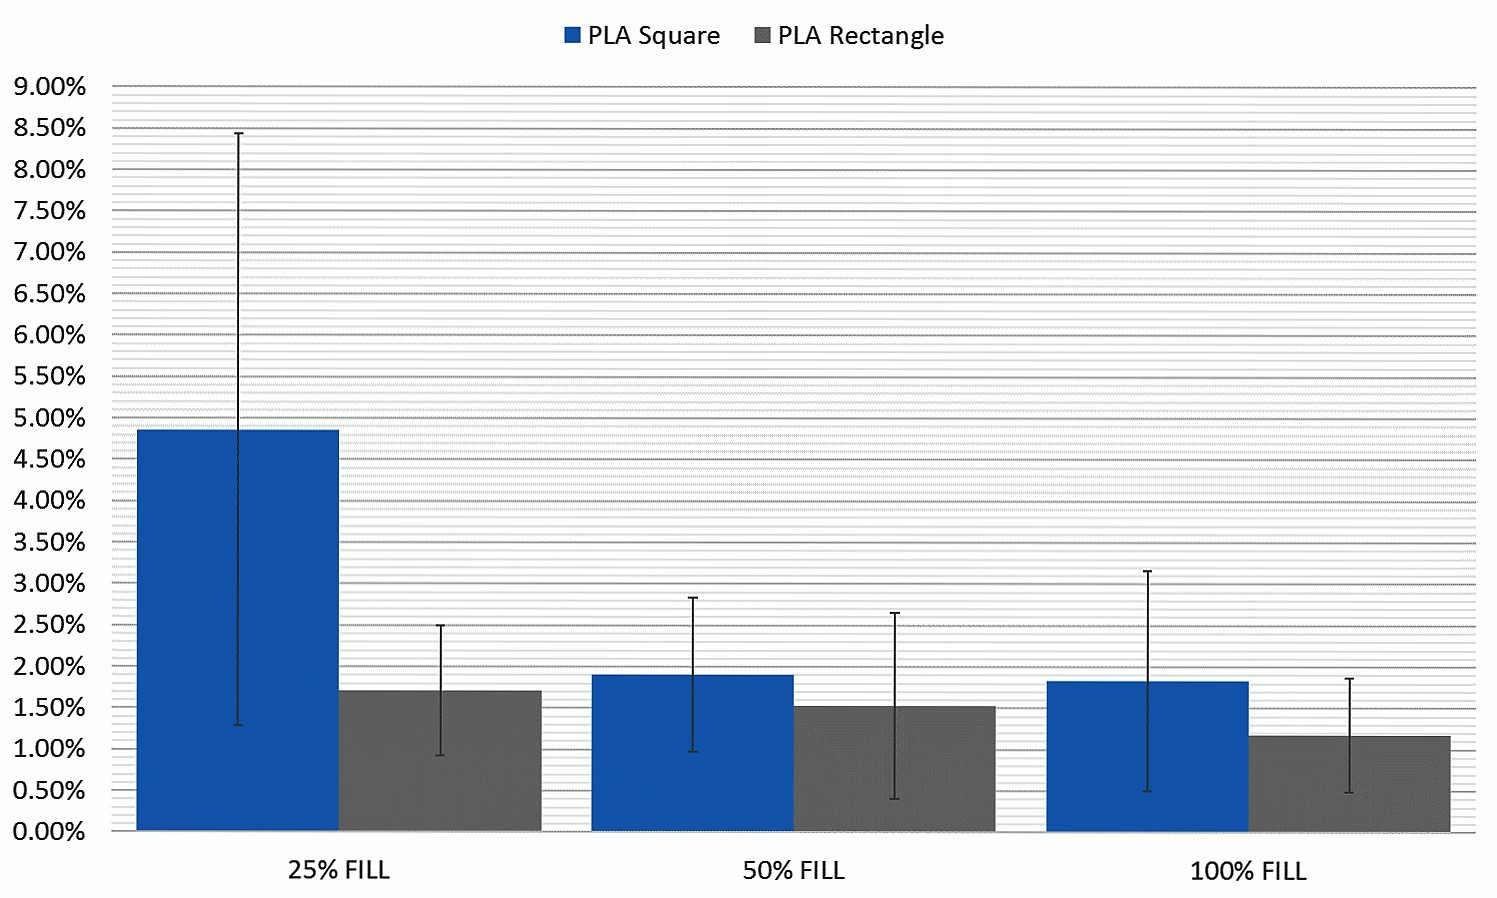
\includegraphics[width=\textwidth]{CHART_PLA_Uncertainty}
		\caption{PLA Uncertainty (\%)}
		\label{fig:PLA_Uncertainty}
	\end{figure}
Similar to table \ref{tab:PLAModAvg}, table \ref{tab:ABSModAvg} contains data for the ABS specimens and the following figures \ref{fig:ABS_Modulus} and \ref{fig:ABS_Uncertanty} illustrate the data for the ABS specimens found in the Appendicies. Of note, ABS Rectangular Specimen \#6 delaminated during testing due to a manufacturing defect, pictured below in figures \ref{fig:Damage1} and \ref{fig:Damage2}.

	\begin{figure} [H]
		\centering
		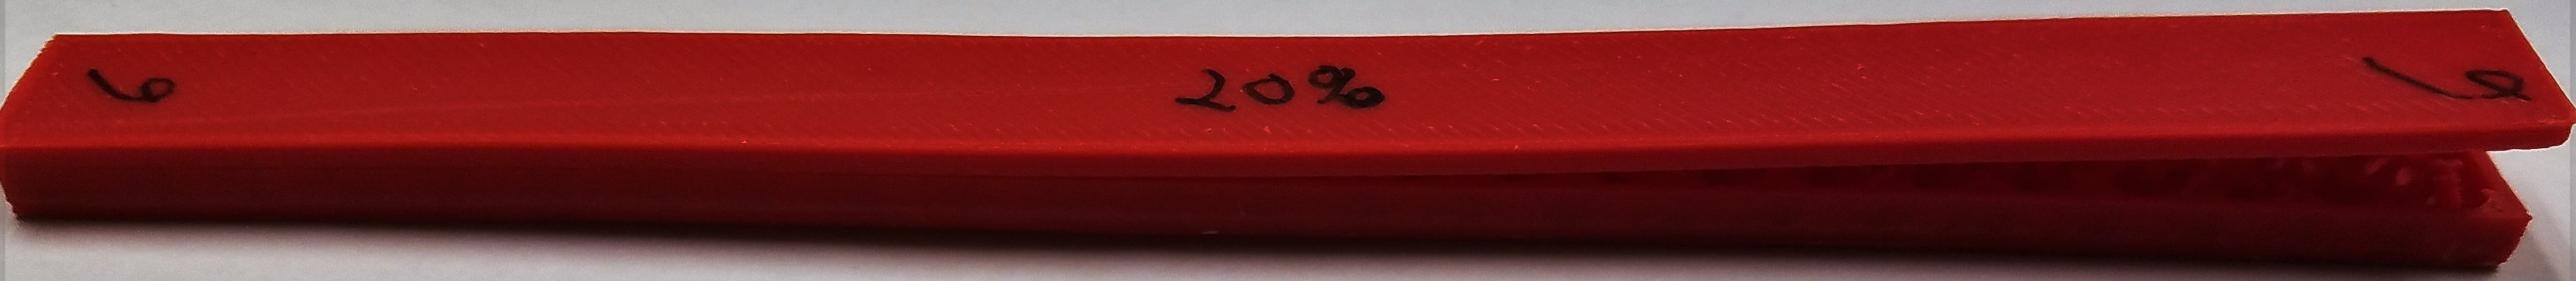
\includegraphics[width=\textwidth]{Damaged_specimen_1}
		\caption{Damaged Specimen Isometric View}
		\label{fig:Damage1}
	\end{figure}
	\begin{figure} [H]
		\centering
		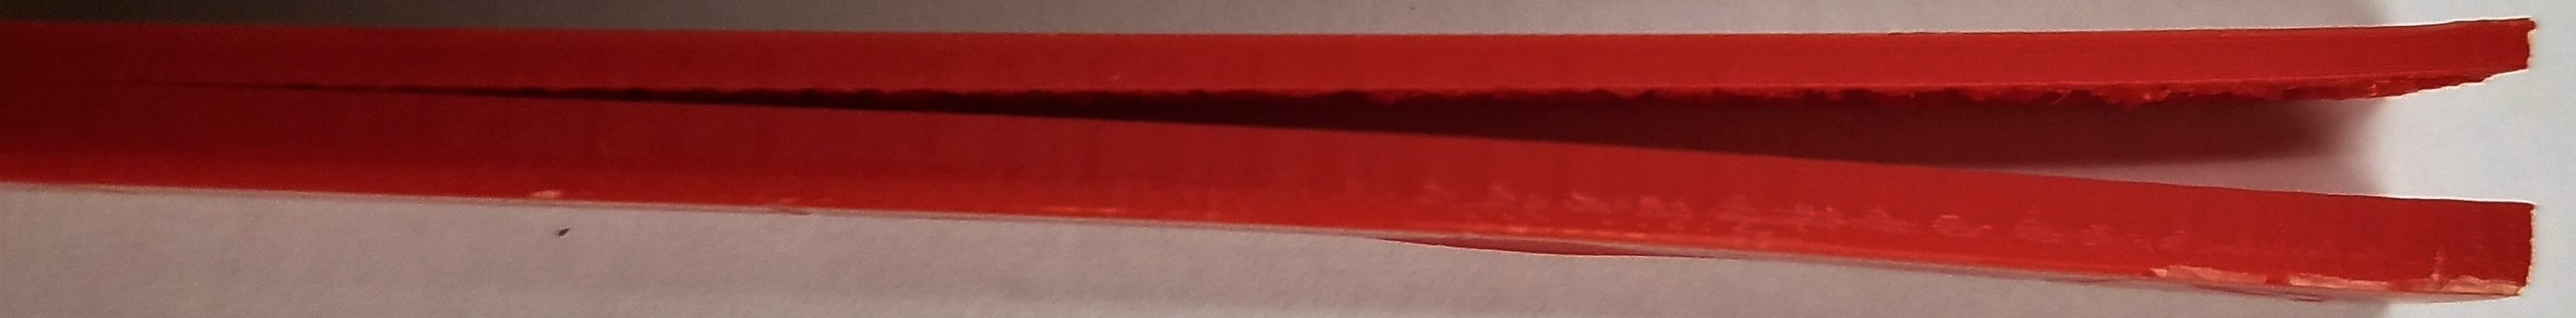
\includegraphics[width=\textwidth]{Damaged_specimen_2}
		\caption{Damaged Specimen Side View}
		\label{fig:Damage2}
	\end{figure}

	\begin{table} [h]
		\centering	
		\begin{tabularx}{\textwidth}{ X X X }
		\noalign{\hrule height 2pt}
			\multicolumn{3}{c}{ABS Modulus of Elasticity Averages} \\ \hline
			SAMPLE & AVG MODULUS (GPa) & UNCERTAINTY (\%) \\ \hline
			SQUARE 25\% & 1.268 & 1.117 \\ 
			SQUARE 50\% & 1.418 & 1.309 \\ 
			SQUARE 100\% & 1.946 & 1.627 \\ 
			RECTANGLE 25\% & 1.439 & 1.282 \\ 
			RECTANGLE 50\% & 1.596 & 1.172 \\ 
			RECTANGLE 100\% & 1.917 & 1.395 \\ \hline
			AVERAGES & 1.597 & 1.317 \\ \hline
		\end{tabularx}
		\caption{Average ABS Beam Specimen Moduli of Elasticity}
		\label{tab:ABSModAvg}
	\end{table}

	\begin{figure} [H]
		\centering
		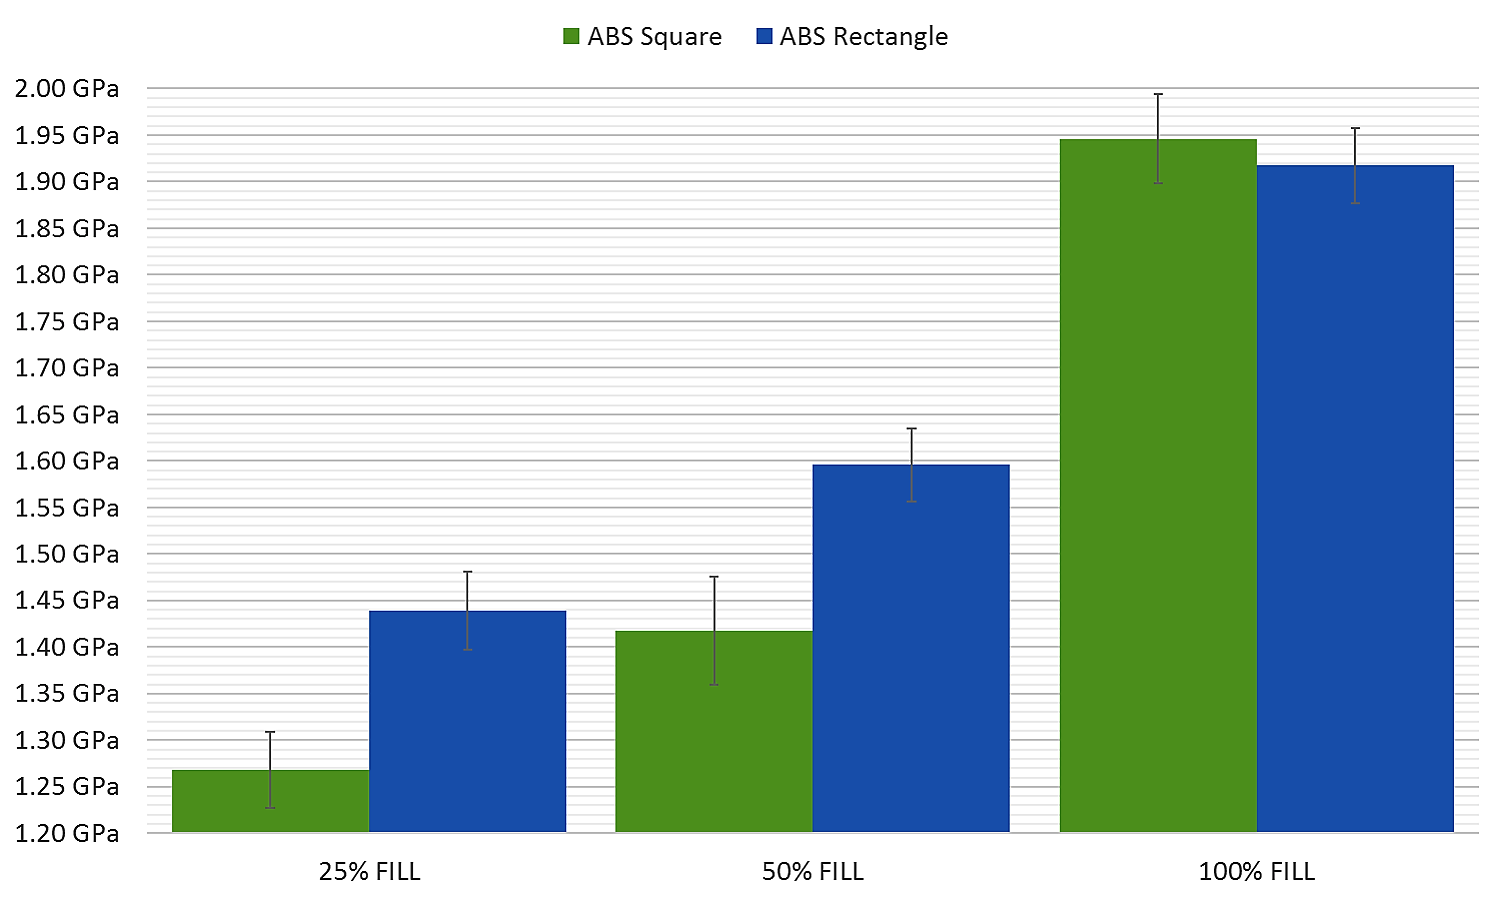
\includegraphics[width=\textwidth]{CHART_ABS_Elasticity}
		\caption{Average ABS Modulus of Elasticity (GPa)}
		\label{fig:ABS_Modulus}
	\end{figure}
	
	\begin{figure} [H]
		\centering
		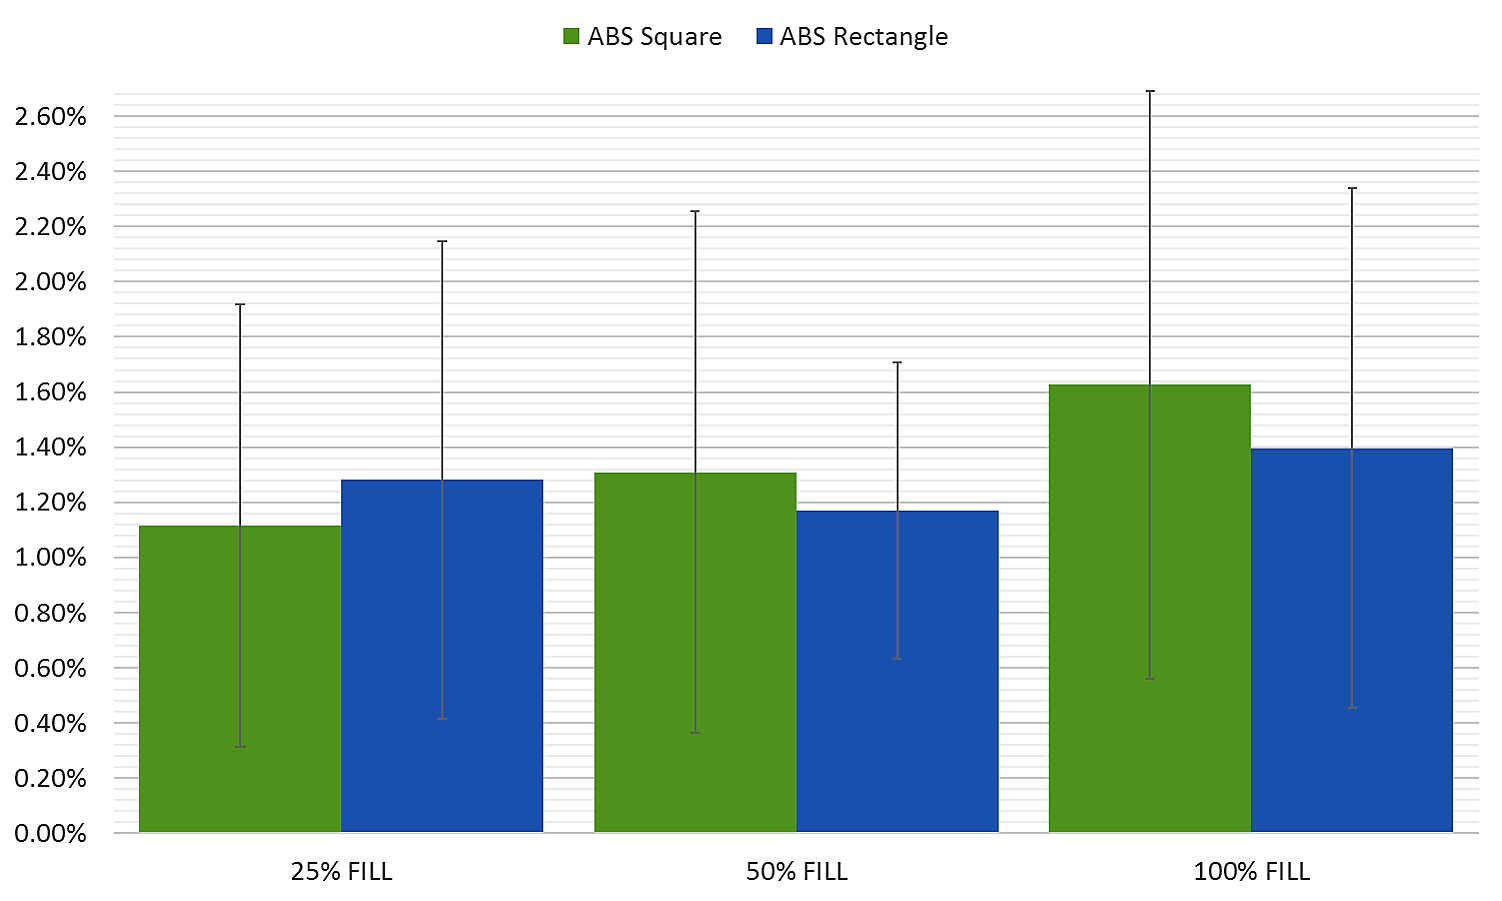
\includegraphics[width=\textwidth]{CHART_ABS_Uncertainty}
		\caption{ABS Uncertainty (\%)}
		\label{fig:ABS_Uncertanty}
	\end{figure}
	
	The experimental data was compared to values found in the literature. As reported in table \ref{tab:PerezABS}, Perez determined the Modulus of Elasticity of the ABS test specimens to be about 1.53 GPa for the specimens printed with their layers oriented parallel to the direction of loading \citep{TorradoPerez2014}. The average modulus of 1.597 GPa found experimentally shows an approximate 4.4\% difference from the ABS modulus reported in the covered literature.
	
	As for the modulus of the PLA specimens, our determined modulus is 2.726 GPa, compared to the 2.159 GPa found by Wendt, et al., noted in table \ref{tab:WendtPLAS} \citep{Wendt2015}. This $\approx 21\%$ difference is most likely due to the fact that Wendt tested single layer specimens as opposed to multi-layer, as well as defects in manufacturing. The single layer specimens were most likely more susceptible to stress concentration due to defects compared to the multi-layer specimens as the printer rotates the orientation of layers as it prints. For example, the first layer may be printed completely in the Y direction while the second layer is at a 45 degree angle to the X and Y axis. This rotation of layers most likely adds to the strength of the objects.

\subsection{Effects of Fill}
	 The effects of the amount of fill used in a 3D printed object seems to be more significant when the amount of infill reaches 100\%, however there is obviously a trend that the amount of infill does increase the strength of an object. There is most likely a point at which increasing the amount in-fill no longer provides a significant increase in strength. However, as displayed by the data below, the average modulus of the 50\% infill is higher than that of the 25\% infill. For all of the sets of specimens, the average modulus of the 25\% and 50\% infill specimens was within $\approx 10\%$, while the minimum difference between the 50\% and 100\% specimens was $\approx 15.5\%$. Table \ref{tab:Infill_Moduli} shows the average results of calculating the modulus of elasticity for the square and rectangular beams at each in-fill density while table \ref{tab:Infill} outlines the percentage differences in the modulus of elasticity between the different infill rates. One can see that the infill density does, in fact, increase the strength of the objects.
	 
	 	 
		\begin{table} [h]
		\centering	
		\begin{tabularx}{.5\textwidth}{ X X }
		\noalign{\hrule height 2pt}
			\multicolumn{2}{c}{EFFECTS OF INFILL} \\ \hline
			SAMPLE SET & AVERAGE MODULUS OF ELASTICITY (GPa) \\ \hline
			PLA 25\% & 2.422\\
			PLA 50\% & 2.519\\
			PLA 100\% & 3.238\\ \hline
			ABS 25\% & 1.267\\
			ABS 50\% & 1.517\\
			ABS 100\% & 1.828\\ \hline
		\end{tabularx}
		\caption{Moduli of Elasticity at Varied Infill Density}
		\label{tab:Infill_Moduli}
		\end{table}	 
		
	 	\begin{table} [h]
		\centering	
		\begin{tabularx}{\textwidth}{ X X }
		\noalign{\hrule height 2pt}
			\multicolumn{2}{c}{EFFECTS OF INFILL} \\ \hline
			SAMPLE SETS & DIFFERENCE IN MODULUS (\%) \\ \hline
			PLA SQUARE 25\%/50\% & 1.979 \\  
			PLA SQUARE 50\%/100\% & 28.619 \\
			PLA SQUARE 25\%/100\% & 27.177 \\ \hline
			PLA RECTANGLE 25\%/50\% & 9.06 \\ 
			PLA RECTANGLE 50\%/100\% & 15.448 \\ 
			PLA RECTANGLE 25\%/100\% & 23.109 \\ \hline
			ABS SQUARE 25\%/50\% & 10.578 \\  
			ABS SQUARE 50\%/100\% & 27.133 \\
			ABS SQUARE 25\%/100\% & 34.841 \\ \hline
			ABS RECTANGLE 25\%/50\% & 9.837 \\  
			ABS RECTANGLE 50\%/100\% & 16.745 \\
			ABS RECTANGLE 25\%/100\% & 24.935 \\ \hline
		\end{tabularx}
		\caption{Effects of Infill Density}
		\label{tab:Infill}
		\end{table}

\section{Phase II: Predicting Behavior \& Investigating Print Orientation}
\subsection{I-Beam Specimen Design}

The references to the XY, XZ, and YZ planes in the following section are discernible from figure \ref{fig:I-Beam_Planes}. To examine the effects of print orientation on printed structures and the uncertainty in predicting the behavior of these objects, I-Beams were printed in three different print orientations pictured in figure \ref{fig:I-Beam_Orientations}.

	\begin{figure} [H]
		\centering
		\caption{I-Beam Plane Orientation}
		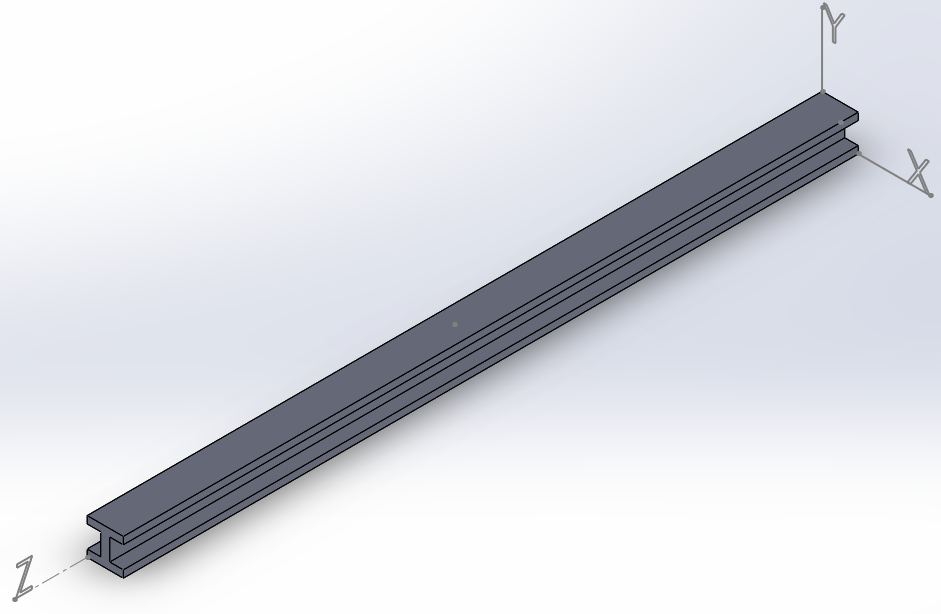
\includegraphics[width=.75\textwidth]{I-BEAM_PLANES}
		\label{fig:I-Beam_Planes}
	\end{figure}
	
	Before experimentation begun, it was theorized that the XZ and YZ beams would behave similarly and that the beams printed with layers in the XY orientation would be the weakest of all of the beams due to the fact that the inter-layer strength is weaker than the strength of the continuous filament layers.
	
	\begin{figure} [H]
		\centering
		\caption{I-Beam Print Orientations}
		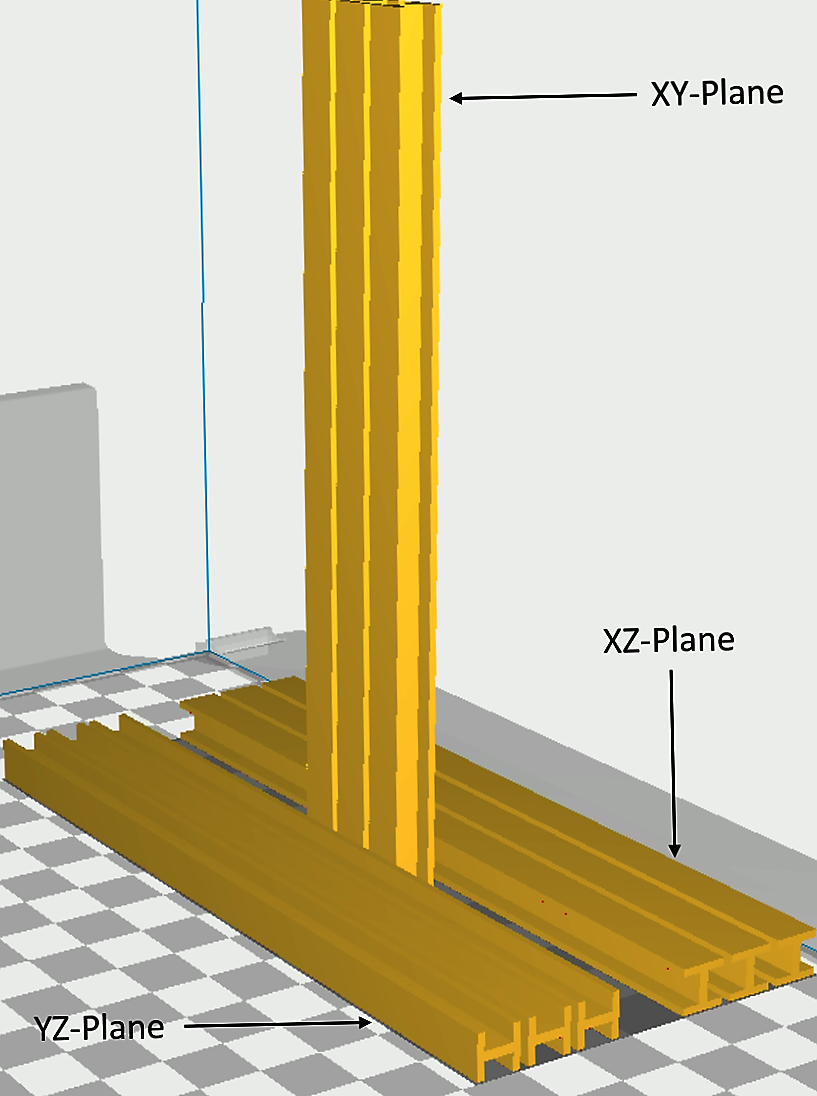
\includegraphics[height=3in]{I-BEAM_CURA}
		\label{fig:I-Beam_Orientations}
	\end{figure}

	Due to the nature of the print orientations, support structure was required to print the XZ and YZ I-Beams which lead to inconsistency in printing close to the nominal beam sizes listed in table \ref{tab:ibeam-nom}. Table \ref{tab:ibeam-dev} notes the average deviation of beams in each print orientation and \ref{tab:ibeam-meas} contains the averaged measurements.
	
	\begin{table} [h]
	\centering
		\begin{tabularx}{\textwidth}{| X | X | X | X | X | X |}
		\hline
			\multicolumn{6}{|c|}{I-Beam Nominal Values} \\ \hline
			\multicolumn{2}{|c|}{BOTTOM FLANGE} & \multicolumn{2}{c|}{TOP FLANGE} & \multicolumn{2}{c|}{WEB}\\ \hline
			 HEIGHT & WIDTH & HEIGHT & WIDTH & HEIGHT & WIDTH \\
			 1.5 & 7.5 & 1.5 & 7.5 & 5 & 1.875 \\ \hline
		\end{tabularx}
		\caption{Nominal I-Beam Measurements}
		\label{tab:ibeam-nom}
	\end{table}
	
	\begin{table} [h]
	\centering
		\begin{tabularx}{\textwidth}{| X | X | X | X | X | X | X |}
		\hline
			\multicolumn{7}{|c|}{I-Beam Measurements} \\ \hline
			& \multicolumn{2}{c|}{BOTTOM FLANGE} & \multicolumn{2}{c|}{TOP FLANGE} & \multicolumn{2}{c|}{WEB}\\ \hline
			Beam & HEIGHT & WIDTH & HEIGHT & WIDTH & HEIGHT & WIDTH \\ \hline
			XY & 1.47 & 7.59 & 1.48 & 7.61 & 4.78 & 1.81 \\ \hline
			XZ & 1.25 & 8 & 1.36 & 7.69 & 4.85 & 1.79 \\ \hline
			YZ & 1.52 & 7.34 & 1.52 & 7.35 & 4.92 & 1.74 \\ \hline
		\end{tabularx}
		\caption{I-Beam Measurements}
		\label{tab:ibeam-meas}
	\end{table}
	
	\begin{table} [h]
	\centering
		\begin{tabularx}{\textwidth}{| X | X | X | X | X | X | X |}
		\hline
			\multicolumn{7}{|c|}{I-Beam Deviation} \\ \hline
			& \multicolumn{2}{c|}{BOTTOM FLANGE} & \multicolumn{2}{c|}{TOP FLANGE} & \multicolumn{2}{c|}{WEB}\\ \hline
			Beam & HEIGHT & WIDTH & HEIGHT & WIDTH & HEIGHT & WIDTH \\ \hline
			XY & 2 & -1.2 & 1.33 & -1.47 & 4.4 & 3.47 \\ \hline
			XZ & 16.67 & -6.67 & 9.33 & -2.53 & 3 & 4.53 \\ \hline
			YZ & -1.33 & 2.13 & -1.33 & 2 & 1.6 & 7.2 \\ \hline
		\end{tabularx}
		\caption{I-Beam Measurement Deviation}
		\label{tab:ibeam-dev}
	\end{table}
	
	When the bending tests were performed on the I-Beam specimens, the top flange of the I beam was facing up regardless of print orientation (the same orientation as the rightmost beams in figure \ref{fig:I-Beam_Orientations}) in order to compare bending for all specimens in the same way. After the data was gathered, the modulus of elasticity of each beam was calculated the same way as in the square and rectangular beams for the linear elastic region captured. For determining the uncertainty, the deformation at 40N was calculated using the average 3.238 GPa modulus of elasticity for 100\% fill PLA and the measured dimensions of the beam and then compared to the actual deformation at $\approx 40N$. 	
	
	The results of the bending tests, listed in table \ref{tab:ibeam_bending_results}, are quite interesting based on previous expectations. The XZ specimens appeared to have the highest modulus of elasticity around 3.134 GPa, which is only $\approx 3.22\%$ lower than the average modulus of 100\% fill PLA beams found in Phase I. The XZ print orientation is the same orientation as the square and rectangular beams, and thus it stands to reason that the I-Beams using the same print orientation have a similar modulus and also shows that print orientation has a significant impact on the strength of the product. The XY samples, which were predicted to be - and are - the weakest have a modulus similar to that of a 50\% infill beam, being only $\approx 2.55\%$ stronger. The YZ beams are in between the strength of the 50\% and 100\% fill beams.

	\begin{table} [h]
		\centering
		\begin{tabularx}{\linewidth}{ | X | X | X | }
		\hline
			Samples & Avg Modulus (GPa) & Uncertainty (\%) \\ \hline
			XY & 2.585 & 26.583 \\
			XZ & 3.134 & 5.199 \\
			YZ & 2.73 & 20.400 \\ \hline
			AVERAGES & 2.816 & 17.394 \\ \hline
		\end{tabularx}
		\caption{I-Beam Bending Test Results}
		\label{tab:ibeam_bending_results}
	\end{table}

It is reasonable to assume that the larger surface area between the layers of the printed beams is the cause of the increased strength due to a larger uniform surface for the next layer to bond to. The following graphs detail the results of individual specimens for the modulus of elasticity and uncertainty in predicting the deformation at 40N.

	\begin{figure} [H]
		\centering
		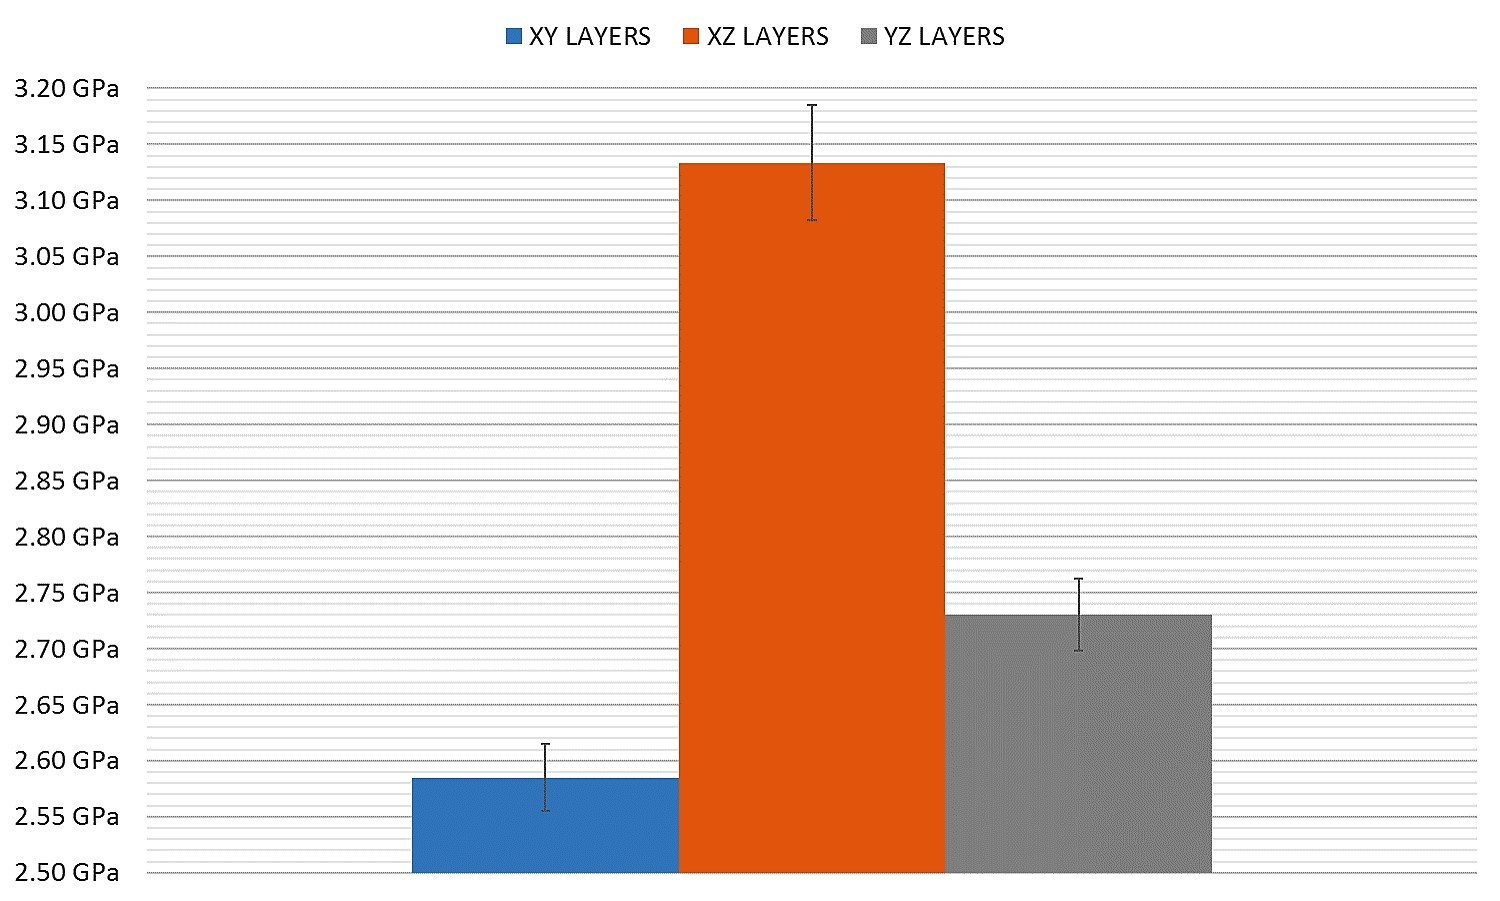
\includegraphics[width=\textwidth]{CHART_I-BEAM_Elasticity}
		\caption{PLA I-Beam Modulus of Elasticity}
		\label{fig:ibeam_Modulus}
	\end{figure}
	
	\begin{figure} [H]
		\centering
		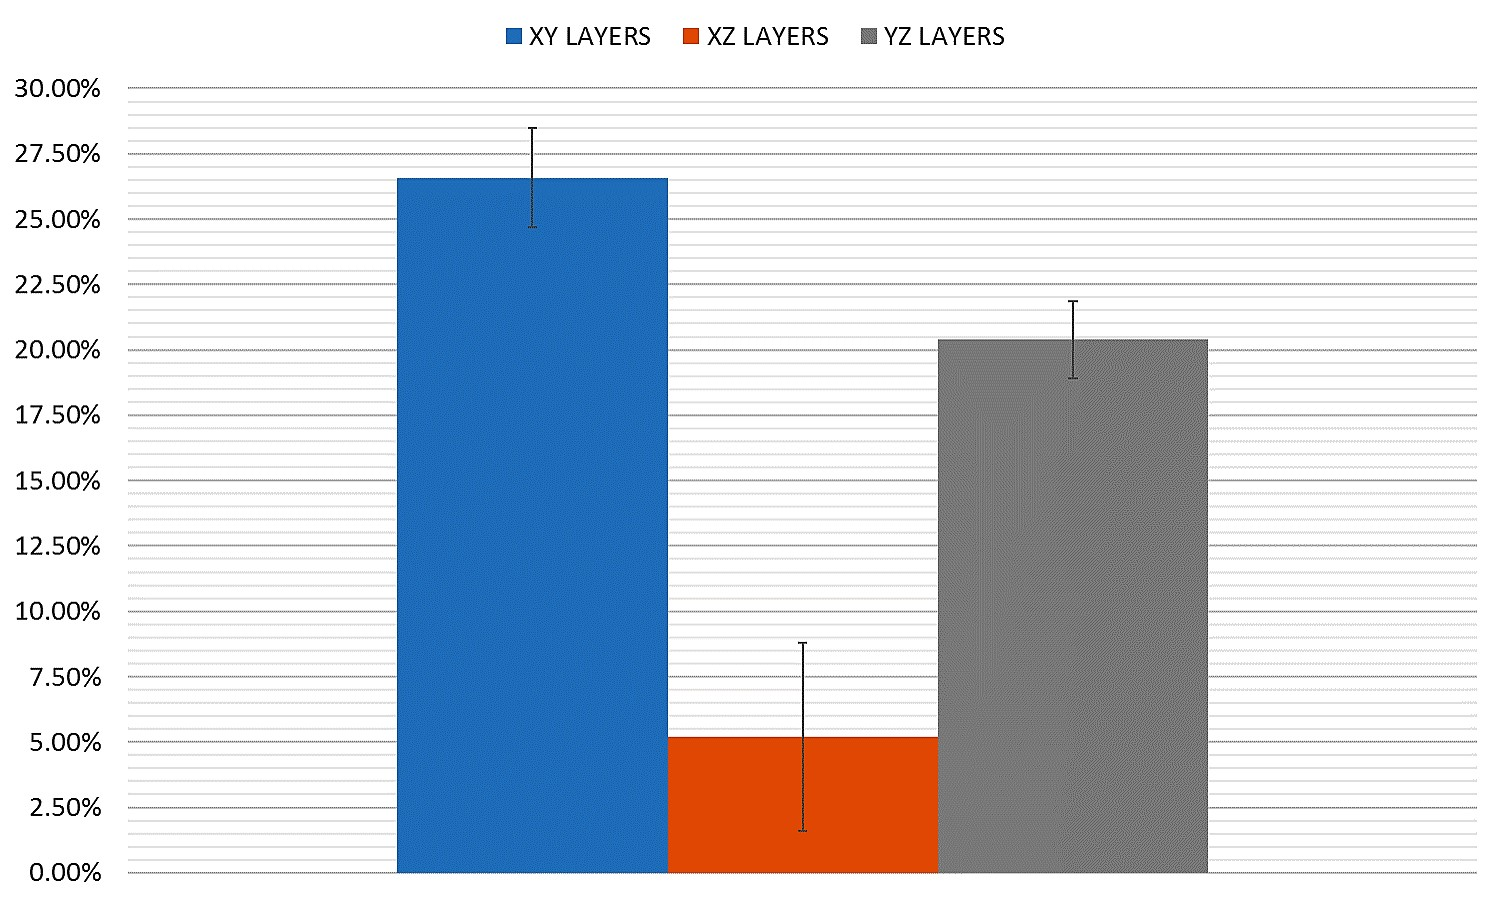
\includegraphics[width=\textwidth]{CHART_I-BEAM_Uncertainty}
		\caption{PLA I-Beam Uncertainty}
		\label{fig:ibeam_Uncertanty}
	\end{figure}

\section{Phase III: Examining UTS Based on Print Orientation}
Phase III was unable to be completed due to scheduling issues with the manufacturing of the grip extensions for the tensile tests. This section is kept here for record keeping and to provide insight into further work.

For our purposes, ASTM D638 was followed with dimensions used for Type I test specimens \citep{ASTMNorma2004} in test specimen design.


\subsection{Design of Grip Extension}
\begin{figure} [H]
\centering
	\caption{\label{ref_label_overall}Grip Extension Clamps}
	\subfloat[Clamp without Bolts]{\label{fig:clamp_no_bolts}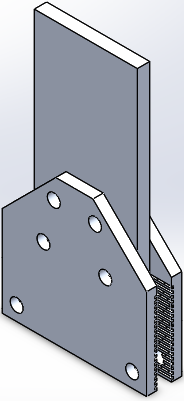
\includegraphics[scale=.7]{Clamp_No_Bolts}}\
	\subfloat[Single Bolt Detail]{\label{fig:clamp_one_bolt}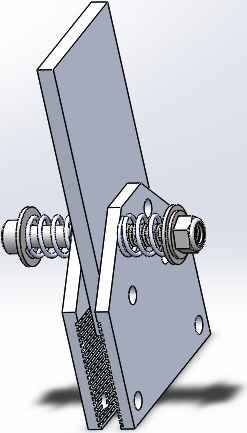
\includegraphics[scale=.65]{Clamp_Single_Bolt}}\
	\subfloat[All Bolts]{\label{fig:clamp_all_bolts}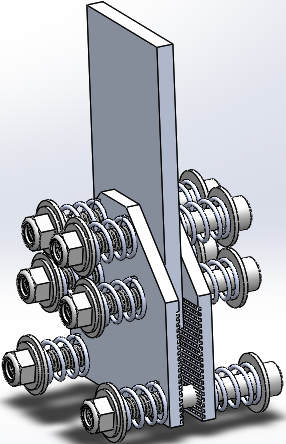
\includegraphics[scale=.65]{Clamp_All_Bolts}}\
\end{figure}

\subsection{Design of Tensile Specimen}

Table \ref{tab:rep_tensile_dimensions} defines the nominal values of the tensile test specimen created in Solidworks. Figure \ref{fig:tens_dim} details the dimensions from \ref{tab:rep_tensile_dimensions} and figure \ref{fig:tens_rend} shows 3D rendering of the specimen taken from Solidworks.

	\begin{table} [H]
		\centering
		\hrule height 2pt 
		\begin{tabularx}{\textwidth}{ | l | X | }
			\multicolumn{2}{|c|}{Type I Tensile Test Specimen Dimensions} \\ \hline
			LO & 200mm\\
			WO & 19mm\\
			L & 57mm\\
			W & 13mm\\
			R & 76mm\\
			T & 3.5mm\\
			G & Unable to provide as no testing was done. \\
		\end{tabularx}
		\hrule height 2pt 
		\caption{Dimensions of Type I Tensile Test Specimens Used}
		\label{tab:rep_tensile_dimensions}
	\end{table}


\begin{figure} [h]
\centering
	\caption{\label{ref_label_overall}Tensile Test Specimens}
	\subfloat[Dimensions Detail]{\label{fig:tens_dim}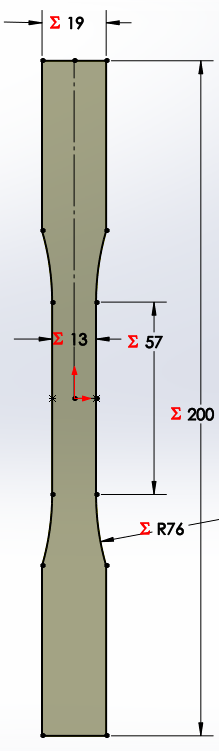
\includegraphics[height=11.5cm]{Tensile_Specimen_Dimensions}}\
	\subfloat[Rendering]{\label{fig:tens_rend}
\includegraphics[height=11.5cm]{Tensile_Specimen_ISO}}\
\end{figure}
\chapter{Conclusions \& Future Work}
\section{Conclusions}
	From the previous chapter, uncertainties observed with predicting the behavior of ABS and PLA specimens are all under a 5\% variance from predicted behavior. It is reasonable to predict the behavior of an object once the material properties have been experimentally determined for a given material and fill density. The uncertainty of the 25\% fill density square specimens was most likely significantly higher than any of the other specimens due to manufacturing defects and , in fact, only specimens 1 and 4 had an uncertainty greater than 6.5\%. It is also worth noting that ABS seemed to be more consistently predictable with a maximum uncertainty of $\approx 4.1\%$ on specimen 100\% \#3 as shown in Appendix B.2.\par
	The density of fill has a significant impact on the strength of an object and shows a clear trend that higher fill density specimens have a larger modulus of elasticity and that 100\% fill objects are significantly stronger than a 25\% or 50\% fill object. This implies that the fill structure does support the loading applied and is not completely dependent on wall thickness. Worthy of note, the standard deviation for the densities seems to be near the same percentage variation for each density and structure. \par
	As shown by the experiments performed on the I-Beam specimens, there is a significant correlation between layer orientation and strength of an object. Table \ref{tab:Layer_Moduli} lists the percentage variance of the average modulus of the sample sets of I-beams from the average modulus of 100\% fill square and rectangular PLA beams. This shows that the strength of the object depends significantly on the orientation of layers with respect to the applied force which implies the bond between the layers is as important as the material itself for the strength. \par

	 	\begin{table} [H]
		\centering	
		\begin{tabular}{ l l }
		\noalign{\hrule height 2pt}
			\multicolumn{2}{c}{EFFECTS OF LAYER ORIENTATION} \\ \hline
			PRINT ORIENTATION & DIFFERENCE IN MODULUS (\%) \\ \hline
			XY & 20.165 \\
			XZ & 3.218 \\
			YZ & 15.674 \\ \hline
		\end{tabular}
		\caption{Effects of Layer Orientation on Modulus}
		\label{tab:Layer_Moduli}
		\end{table}


	The reason that modulus of elasiticy that was found for PLA is high in the performed experiments when compared to Wendt's data is most likely due to having multi-layer objects and the strength that is provided by the bonding between the layers shown by the data from the I-beam experiments. This along with the rotation of the printing path that the slicing software performs allows defects to not have as much of an effect as with a single layer specimen. \par
	The experiments performed here clearly show that the layer orientation significantly impacts the strength of an object. While products may not be constructed from ABS or PLA plastics, the same limitations are likely arise. More research is necessary, but it is logical to conclude that the layer orientation will be a significant factor to consider in future applications such as medical implants or structural components. Another trend of note is that the surface area between layers may play a more significant role than expected as shown by figures \ref{fig:PLA_Modulus} and \ref{fig:ABS_Modulus}. There is a trend shown that the rectangular specimens tend to have a higher modulus of elasticity than the square counterparts, however this diminishes as the fill density nears 100\% fill. This is a point of interest that should be investigated.\par


\section{Proposed Work}
	One variable that should be studied is the diminishing returns on increasing the amount of fill density and determine the amount of fill that would be most economical to use. For further investigation it would be beneficial to observe the shear strength of layers for different fill densities and layer orientations to determine how the surface area of a layer effects the shear strength. \par
	Table \ref{tab:Print_settings} lists the settings used on the printer that are referenced in this section. Based on the data from Phase I fill density has an effect on the modulus of elasticity, however it appears that the wall thickness provides a large amount of strength to the structure. Varying the wall thickness for 25\% and 50\% fill to study the effects on the modulus of elasticity is suggested. Similarly, varying layer height could also significantly impact the strength of an object. Print speed is a variable that should be examined as the rate at which layers cool is dependent on how quickly material is deposited. As shown in the study by Wang, a slower print speed tended to cause a more uniform structure and increased strength \citep{Wang2016}. Print consistency, or the amount of variance between prints and the design should be minimized in order to provide a considerable comparison between samples. \par
	

	 	\begin{table} [H]
		\centering	
		\begin{tabular}{ l l }
		\noalign{\hrule height 2pt}
			Print Speed & $60\frac{mm}{s}$\\
			Wall Thickness & 0.8mm \\
			Layer Height & 0.1mm \\ \hline
		\end{tabular}
		\caption{Printer Settings}
		\label{tab:Print_settings}
		\end{table}
	
	Once more understanding of how the printing process affects the final products, inducing defects would be the next major step in determining how these structures would behave. Voids, delamination and shifts in layers seemed to be the most common defects from both the literature and first hand experience printing the specimens for this study.
%%%%%%%%%%%%%%%%%%%%%%%%%%%%%%%%%%%%%%%%%%%%%%%%%%%%%%%%%%%%%%%
% Appendices
%
% Because of a quirk in LaTeX (see p. 48 of The LaTeX
% Companion, 2e), you cannot use \include along with
% \addtocontents if you want things to appear the proper
% sequence.
%%%%%%%%%%%%%%%%%%%%%%%%%%%%%%%%%%%%%%%%%%%%%%%%%%%%%%%%%%%%%%%
\appendix
\titleformat{\chapter}[display]{\fontsize{30}{30}\selectfont\bfseries\sffamily}{Appendix \thechapter\textcolor{gray75}{\raisebox{3pt}{|}}}{0pt}{}{}
% If you have a single appendix, then to prevent LaTeX from
% calling it ``Appendix A'', you should uncomment the following two
% lines that redefine the \thechapter and \thesection:
%\renewcommand\thechapter{}
%\renewcommand\thesection{\arabic{section}}
\Appendix{Code} \label{app:code}
\lstinputlisting[language=Python, breaklines=true]{./Material/Appendices/stepper.py}
\Appendix{Square Beam Data} \label{app:square}
\section{Measurements}
	\begin{center}
		\LTXtable{\textwidth}{./Material/Appendices/Dimensions_Square.tex}
	\end{center}
\newpage
\section{ABS Bending Data}
	\begin{center}
		\LTXtable{\textwidth}{./Material/Appendices/Data_ABS_Square.tex}
	\end{center}
\newpage
\section{PLA Bending Data}
	\begin{center}
		\LTXtable{\textwidth}{./Material/Appendices/Data_PLA_Square.tex}
	\end{center}
\Appendix{Rectangular Beam Data} \label{app:rectangle}
\section{Measurements}
	\begin{center}
		\LTXtable{\textwidth}{./Material/Appendices/Dimensions_Rectangle.tex}
	\end{center}
\newpage
\section{ABS Bending Data}
	\begin{center}
		\LTXtable{\textwidth}{./Material/Appendices/Data_ABS_Rectangle.tex}
	\end{center}
\newpage
\section{PLA Bending Data}
	\begin{center}
		\LTXtable{\textwidth}{./Material/Appendices/Data_PLA_Rectangle.tex}
	\end{center}
\Appendix{I-Beam Data} \label{app:ibeams}
\section{Measurements}
	\begin{center}
		\LTXtable{\textwidth}{./Material/Appendices/Dimensions_I-Beams.tex}
	\end{center}
\newpage
\section{Bending Data}
	\begin{center}
		\LTXtable{\textwidth}{./Material/Appendices/Data_I-Beams.tex}
	\end{center}
%%%%%%%%%%%%%%%%%%%%%%%%%%%%%%%%%%%%%%%%%%%%%%%%%%%%%%%%%%%%%%%
% ESM students need to include a Nontechnical Abstract as the %
% last appendix.                                              %
%%%%%%%%%%%%%%%%%%%%%%%%%%%%%%%%%%%%%%%%%%%%%%%%%%%%%%%%%%%%%%%
% This \include command should point to the file containing
% that abstract.
%\include{nontechnical-abstract}
%%%%%%%%%%%%%%%%%%%%%%%%%%%%%%%%%%%%%%%%%%%
} % End of the \allowdisplaybreak command %
%%%%%%%%%%%%%%%%%%%%%%%%%%%%%%%%%%%%%%%%%%%

%%%%%%%%%%%%%%%%
% BIBLIOGRAPHY %
%%%%%%%%%%%%%%%%
% You can use BibTeX or other bibliography facility for your
% bibliography. LaTeX's standard stuff is shown below. If you
% bibtex, then this section should look something like:
	\nocite{*}
	\begin{singlespace}
%	\bibliographystyle{GLG-bibstyle}
	\bibliographystyle{plainnat}
	\addcontentsline{toc}{chapter}{Bibliography}
	\bibliography{./BibTeX/Thesis}
	\end{singlespace}

%\begin{singlespace}
%\begin{thebibliography}{99}
%\addcontentsline{toc}{chapter}{Bibliography}
%\frenchspacing

%\bibitem{Wisdom87} J. Wisdom, ``Rotational Dynamics of Irregularly Shaped Natural Satellites,'' \emph{The Astronomical Journal}, Vol.~94, No.~5, 1987  pp. 1350--1360.

%\bibitem{G&H83} J. Guckenheimer and P. Holmes, \emph{Nonlinear Oscillations, Dynamical Systems, and Bifurcations of Vector Fields}, Springer-Verlag, New York, 1983.

%\end{thebibliography}
%\end{singlespace}

\backmatter

% Vita
%\vita{SupplementaryMaterial/Vita}

\end{document}

